\documentclass{fmb-thesis}

\makeglossaries

\usepackage{thesis/glossary/glossary}
\addbibresource{thesis/bibliography/pensums.bib}
\addbibresource{thesis/bibliography/python.bib}
\addbibresource{thesis/bibliography/uniandes.bib}
\addbibresource{thesis/bibliography/visualization.bib}
\addbibresource{thesis/bibliography/otros.bib}

\usepackage[Bjornstrup]{fncychap}

\renewcommand{\listtablename}{Índice de Tablas}

\begin{document}

\definecolor{cover_gray}{RGB}{229 229 229}
\begin{titlepage}
	
\includegraphics[width=0.7\textwidth]{thesis/assets/uniandes.png}
	\vskip1.5cm
	\begin{tikzpicture}[remember picture, overlay]
		\fill [cover_gray, opacity=1] (current page.west|-0,0) rectangle (current page.east|-0,-500);
	\end{tikzpicture}
	\raggedright
	\vskip2cm
	{%
		\fontsize{22}{26.4}\selectfont
		\bfseries
		\sffamily
		Desarrollo del Perfil del estudiante\\
		dentro de No estás solo
		\par
	}
	\vskip2cm
	{%
		\fontsize{17}{17}\selectfont
		\sffamily
		Federico Melo Barrero\\
		\fontsize{12}{17}\selectfont
		f.melo@uniandes.edu.co
		\par
	}
	\vskip0.7cm
	{%
	\fontsize{14}{17}\selectfont
	\sffamily
	\raggedright
	\noindent
	Directora: \fontsize{16}{17}\selectfont Marcela Hernández Hoyos, Ph.D.\\
	\fontsize{12}{17}\selectfont
	\textit{Vicedecana de Asuntos Estudiantiles $\mid$ Facultad de Ingeniería} \\
	\fontsize{12}{17}\selectfont
	marc-her@uniandes.edu.co
	\par
	}
	\vfill
	{%
		\fontsize{12}{14}\selectfont
		\sffamily
		\raggedright
		\noindent Proyecto de grado presentado como requisito parcial para optar al título de:\\
		\fontsize{13}{16}
		\textbf{Ingeniero de Sistemas y Computación}
		\par
	}
	\vskip0.5cm
	{%
	\fontsize{13}{16}\selectfont
	\sffamily
	Bogotá D.C., Colombia
	\par
	}
	\vskip1cm
\end{titlepage}


\section*{\centering Resumen}

\begin{spacing}{1.5}
El presente proyecto de grado describe el desarrollo del Perfil del estudiante al interior de la plataforma web No estás solo. El Perfil del estudiante consiste de un conjunto de visualizaciones interactivas que presentan información académica y contextual sobre cada estudiante de la Universidad de los Andes. Dirigido principalmente a profesores en su rol como consejeros, su uso se extendió a estudiantes, coordinadores y administrativos, quienes encontraron valiosa la información para procesos de consejería y toma de decisiones. Este documento detalla todo lo asociado con la construcción del Perfil: inicia por el contexto que suscitó su creación; luego, expone minuciosamente el desarrollo técnico del módulo, adentrándose en el diseño e implementación de las capas de datos, lógica y presentación, y abordando las tecnologías y prácticas de ingeniería de software empleadas; finalmente, exhibe el Perfil del estudiante en acción como producto final del proyecto.
\end{spacing}

\section*{\centering Abstract}

\begin{spacing}{1.5}
This thesis project describes the development of the Student Profile within the web platform No estás solo. The Student Profile consists of a set of interactive visualizations that present academic and contextual information about each student at the Universidad de los Andes. Initially designed for professors in their role as academic advisors, its use expanded to students, coordinators, and administrative staff, who found the information valuable for counseling processes and decision-making. This document outlines all aspects related to the creation of the Student Profile: it begins by providing the context that motivated its development; then, it thoroughly details the technical construction of the module, delving into the design and implementation of the data, business logic, and presentation layers, as well as the technologies and software engineering practices employed. Finally, it showcases the Student Profile in action as the final product of the project.
\end{spacing}

\chapter*{Agradecimientos}

Mi participación en este proyecto fue meramente fortuita. A inicios de 2024, cuando Nicolás Carvajal y Mariana Ruiz me recomendaron como desarrollador a Marcela Hernández, Vicedecana de Asuntos Estudiantiles de la Facultad de Ingeniería, yo no tenía idea de cuál sería su encomienda. Marcela compartió conmigo su sueño: el Perfil del estudiante. A pesar de que la información del estudiantado existía, estaba dispersa y accederla era tortuoso. La centralización y democratización de esa información entre profesores y administrativos, que entonces parecía un objetivo casi utópico, prometía beneficios inconmensurables: decisiones informadas, fundamentadas en datos, y consejerías verdaderamente personalizadas.

No tomó mucho de parte de Marcela para convencerme de involucrarme cuando vislumbré el impacto del proyecto. En su momento, sin embargo, subestimé la magnitud. Aunque en pocos meses desplegamos la primera versión del Perfil del estudiante, mi compromiso inicial de seis meses se convirtió en un año de trabajo arduo, enfrentando retos técnicos que abarcaron todas las capas del desarrollo de software —datos, lógica de negocio, presentación y despliegue—, y viviendo la gratificación de contribuir a un proyecto que impacta directamente la vida de los estudiantes de la Universidad de los Andes.

Yo creo que era eso último lo que nos mantenía despiertos hasta las cuatro de la mañana, a mí y a Santiago Martínez, quien a partir de agosto de 2024 asumió la responsabilidad de la capa de datos.

Este proyecto recoge, entonces, mi trabajo como desarrollador en la Vicedecanatura durante mi último año de carrera, pero también representa el cierre simbólico de mi recorrido académico en la Universidad. Por esta razón, no quiero limitar estos agradecimientos únicamente a quienes contribuyeron directamente al desarrollo del Perfil del estudiante, sino extenderlos a todas las personas que, de una u otra manera, han sido imprescindibles en mi formación académica y personal.

El año 2024 fue un periodo de muchos cambios y de trabajo diligente. Además de trabajar en este proyecto, desempeñé el rol de monitor de investigación en el proyecto Cupi2, enfocado en mejorar la enseñanza de programación en la Universidad; trabajé como desarrollador de software en el equipo de analítica de datos de la multinacional canadiense Caseware; y completé las materias necesarias para graduarme como Ingeniero de Sistemas y Computación. Este esfuerzo se vio recompensado con los mejores resultados académicos de mi trayectoria y me permitió culminar mis estudios con el Promedio General Acumulado más alto de la Facultad de Ingeniería en los últimos quince años.

Eso, por supuesto, no hubiese sido posible solo. Antes que a nadie, quiero agradecer profundamente a Angélica, William y Sebastián: mi familia. Su crianza amorosa moldeó mi persona y su apoyo incondicional ha sido el cimiento de mis logros. A ellos les debo este y todos mis proyectos.

En segundo lugar, debo un enorme agradecimiento a mis amigos más cercanos. Ellos son un pilar fundamental en mi vida y en mi felicidad, y contribuyen constantemente a una ya extensa colección de momentos inolvidables. A David Fuquen, Santiago Martínez y Andrés Guerrero; y a Laura Ramírez, Laura Córdoba, Mariana Rodríguez y Sarah Pérez: gracias por estar en mi vida. Sin esos dos conjuntos de personas, el camino no hubiese sido tan agradable, por decir lo menos.

Extiendo también mi gratitud a todas las personas que, a lo largo de los años, han invertido su tiempo, conocimiento y esfuerzo en mi educación. Eso incluye a todos quienes fueron partícipes de mi formación tanto en el Colegio San Carlos como en la Universidad de los Andes. No ignoro el inmenso privilegio que constituye haber estudiado en las mejores instituciones educativas del país y haber contado con mentores extraordinarios. Mis agradecimientos más profundos van para Jaime Rueda Moreno y Héctor Carranza Granados, quienes me enseñaron a estudiar; y para Nicolás Rincón Sánchez y Alejandro Arturo Pérez Ramírez, quienes me forzaron a hacerlo rigurosamente.

También quiero destacar a algunas personas que confiaron en mi potencial y me brindaron oportunidades que resultaron ser puntos de inflexión en mi formación. En particular, a Iván David Salazar Cárdenas, quien apostó por mí en el proyecto Cupi2; y a José Joaquín Bocanegra García, quien despertó mi interés por el desarrollo web y auspició mi primera experiencia como desarrollador de software.

Finalmente, quisiera agradecer a mis colegas en la Vicedecanatura. A Mariana y Nicolás, quienes mantienen y extienden el resto de No estás solo; a Catalina, Manuel y (nuevamente) Santiago, cuya pericia en ingeniería de datos hizo posible el desarrollo del proyecto; a Oscar, siempre pendiente de todo; y, por supuesto, a Marcela, quien confió en mí, me dio esta oportunidad única de generar impacto mediante mi conocimiento y me acompañó durante todo el proceso.

A todos los acá mencionados y quienes no lo están, pero que han sido parte de mi vida en los últimos años, gracias por acompañarme y contribuir a que esta etapa de mi vida sea tan significativa. Los resultados son muy buenos y les pertenecen a ustedes.

\vspace*{\fill} % Vertically center the content
\begin{flushright}
	\textit{Big Brother is watching you.} \\[1em]
	---George Orwell, \textit{Nineteen Eighty-Four}
\end{flushright}


\tableofcontents

\listoffigures
\addcontentsline{toc}{chapter}{Índice de Figuras}

\listoftables
\addcontentsline{toc}{chapter}{Índice de Tablas}

\chapter{Introducción}

\begin{resumen}
	\gls{NES} es una plataforma web desarrollada por la Universidad de los Andes que centraliza sus recursos y servicios. Este proyecto se enfoca en el Perfil del estudiante: un módulo que complementa esta plataforma al proporcionar información académica y socioeconómica del estudiantado, previamente ausente, pero esencial para mejorar las consejerías a estudiantes y las decisiones administrativas. 
	
	El módulo se construye mediante una arquitectura de software \textit{three-tier}, que se detalla en los siguientes capítulos.
\end{resumen}

\section{Contexto}

La Universidad de los Andes es una institución educativa de gran renombre, reconocida por estar a la vanguardia de la educación en Colombia, su permanente excelencia académica y su férreo compromiso con la formación integral de sus estudiantes. En aras de propulsar el éxito de sus estudiantes en todo ámbito, la Universidad realiza un esfuerzo constante por ofrecer servicios y recursos que fomenten el desarrollo académico, social, personal y profesional de los alumnos, así como el bienestar de la comunidad universitaria en general.

\subsection{La plataforma \textit{No estás solo}}

En los últimos dos años, la Vicedecanatura de Asuntos Estudiantiles de la Universidad de los Andes identificó dos dolencias significativas concernientes al estudiantado y al profesorado, respectivamente. La primera, consiste en el desconocimiento por parte de los estudiantes de la inmensa cantidad de recursos y servicios de apoyo que la Universidad pone a su disposición en pos de su progreso académico, social, personal y profesional. La segunda, radica en la dificultad y falta de recursos que tenían los profesores a la hora de ejercer su labor como consejeros en apoyo a los estudiantes.

Como herramienta para subsanar estas dolencias, la Vicedecanatura ha impulsado el desarrollo y la extensión de una aplicación web: \textit{No estás solx} (en adelante, \gls{NES}). Esta plataforma fue concebida por la Vicedecanatura de Asuntos Estudiantiles de la Facultad de Ingeniería como una solución integral para garantizar que todos los miembros de la comunidad, especialmente los estudiantes, puedan acceder de manera centralizada y clara a todos los recursos y servicios disponibles.

Desde la perspectiva del estudiantado, \gls{NES} centraliza el acceso a todas las herramientas que fomentan su éxito académico, personal y profesional. Esto incluye información sobre eventos académicos y culturales, procesos y solicitudes administrativas, y servicios de apoyo como consejerías y tutorías. Sumado a eso, facilita el acceso de cada estudiante a su red de apoyo, compuesta por profesores consejeros, coordinadores académicos y otros profesionales de la Universidad. Toda esta información se encontraba dispersa en las distintas plataformas de la Universidad, lo que dificultaba su acceso y su uso conjunto. Esto suponía un reto importante para los estudiantes, quienes debían navegar entre múltiples sistemas y portales para encontrar la información que necesitaban, además de constituir una barrera de entrada significativa para los estudiantes menos experimentados.

Para los profesores y otros usuarios administrativos, \gls{NES} constituye una herramienta que facilita su labor como consejeros y mejora su capacidad de toma de decisiones. La plataforma incluye una base de preguntas frecuentes y guías para poder orientar a los estudiantes en dificultades académicas, personales o financieras. Finalmente, para los coordinadores académicos, \gls{NES} contribuye a descongestionar las solicitudes frecuentes poniendo a disposición herramientas de autogestión que permiten que los estudiantes resuelvan problemas simples por sí mismos, lo cual optimiza el uso del tiempo en las coordinaciones.

\subsection{La necesidad del Perfil del estudiante}

\gls{NES} representa un avance significativo en la centralización y claridad de los recursos y servicios ofrecidos por la Universidad. Sin embargo, previo a la implementación del Perfil del estudiante, los profesores y administrativos enfrentaban desafíos al intentar ofrecer consejerías personalizadas o tomar decisiones informadas. La información sobre los estudiantes estaba dispersa en múltiples sistemas y formatos, lo que dificultaba tener una visión integral de su contexto académico y socioeconómico de forma oportuna.

El Perfil del estudiante surge como una respuesta directa a esta necesidad. Este módulo se integra dentro de \gls{NES} para ofrecer una herramienta que:
\begin{itemize}
	\item Centralice y organice la información relevante sobre los estudiantes.
	\item Presente esta información de manera intuitiva, clara e inmediatamente accesible, sin sacrificar la exhaustividad.
	\item Facilite a profesores y administrativos brindar consejerías personalizadas y tomar decisiones basadas en datos.
\end{itemize}

Con estas características, el Perfil del estudiante no solo mejora la experiencia de los usuarios de \gls{NES}, sino que también fortalece su capacidad de impacto al abordar de manera directa las problemáticas identificadas por la Vicedecanatura de Asuntos Estudiantiles.

\section{Objetivos}

El objetivo general de este proyecto es construir el Perfil del estudiante.

Más específicamente, el objetivo radica en proporcionar a todo el estudiantado y al profesorado de la Universidad de los Andes una herramienta digital que les permita consultar información relacionada con el desempeño académico actual y pasado, así como con el contexto socioeconómico, de los estudiantes de la Universidad.

\subsection{Objetivos específicos}

El objetivo general enunciado recién se desglosa en los siguientes objetivos específicos:
\begin{itemize}
	\item Desarrollar una herramienta de software que permita acceder a la información académica de los estudiantes de la Universidad de los Andes, permitiendo su interacción con una aplicación web, preferiblemente basada en los lineamientos de un \gls{API REST}.
	\item Diseñar e implementar un módulo de la aplicación web \gls{NES} que extraiga y exhiba la información académica de cualquier estudiante de la Universidad de los Andes. Realizar la distinción entre la forma en la que se presenta la información para estudiantes de pregrado y estudiantes de posgrado, en particular, distinguir entre los resultados de un mismo estudiante en su pregrado y en su posgrado, teniendo completa trazabilidad de su trayectoria académica cuando sea el caso.
	\item Conectar el módulo con la navegación y funcionalidades ya existentes en la aplicación web \gls{NES}, de forma que cada estudiante pueda tener acceso a su información académica (mas no a la de otros estudiantes), cada profesor consejero pueda tener acceso a la información académica de sus estudiantes aconsejados y otros usuarios específicos, determinados por la Vicedecanatura, puedan tener acceso a la información académica de los estudiantes que les conciernan.
	\item Garantizar la integridad y seguridad de la información académica de los estudiantes de la Universidad de los Andes, tanto informáticamente como en su presentación, de forma que se cumpla con la normativa de protección de datos personales y de información académica de la Universidad.
\end{itemize}

\subsection{Resultados esperados}

El presente proyecto se puede dar por culminado una vez se satisfaga el siguiente conjunto de resultados:
\begin{itemize}
	\item Existencia de un módulo de la aplicación web \gls{NES} que permita a cada estudiante de la Universidad de los Andes, tanto de pregrado como de posgrado, consultar información relacionada con su desempeño académico.
	\item Existencia de un módulo de la aplicación web \gls{NES} que permita a cada profesor de la Universidad de los Andes consultar información relacionada con el desempeño académico de cada uno de sus estudiantes aconsejados, de forma individual.
	\item Existencia de un módulo de la aplicación web \gls{NES} que permita a usuarios específicos, como decanos, directores de programas u otros directivos de la Universidad de los Andes, consultar información relacionada con el desempeño académico de los estudiantes de la Universidad que les conciernan.
\end{itemize}

\section{Arquitectura general del sistema}

El Perfil del estudiante se construye sobre una arquitectura de software \text{three-tier}, dividida en tres capas: la capa de datos, la capa de lógica y la capa de presentación. Los próximos tres capítulos se centran cada uno en una de estas capas. Esta organización modular facilita el desarrollo, mantenimiento y escalabilidad del sistema, porque permite una separación clara de responsabilidades.

La capa de datos es el cimiento del sistema, encargándose de la extracción, transformación y carga (\gls{ETL}) de los datos. Esta capa garantiza que la información proveniente de diversas fuentes sea estructurada y almacenada de manera consistente, preparándola para ser utilizada por las capas superiores (e, incluso, por otras dependencias de la Universidad para análisis de otros tipos). En esta etapa, los datos fluyen desde sus fuentes originales hasta ser almacenados clasificados semánticamente, como se describe detalladamente en el Capítulo \ref{ch:datos}.

La capa de lógica, descrita en el Capítulo \ref{ch:logica}, actúa como el cerebro del sistema. Aquí, los datos procesados se transforman en recursos, que son expuestos por una \gls{API REST}. Esta capa se ocupa del cumplimiento de las reglas de negocio, es decir, de las restricciones de la vida real y del contexto de la Universidad que deben ser impuestas a los datos. Además, define la interfaz a través de la cual la capa de presentación (y potencialmente otros servicios web similares) puede interactuar con los datos. La capa de lógica es completamente independiente de la capa de datos; es posible cambiar por completo la implementación de cualquiera de las dos capas, sin que sea necesario modificar la otra, mientras se mantenga la interfaz entre ambas.

Por último, la capa de presentación, descrita en el Capítulo \ref{ch:presentacion}, es la cara visible del sistema para los usuarios finales. Su objetivo principal es proporcionar una experiencia de usuario que sea intuitiva, interactiva y accesible, complementada por un diseño visual atractivo. Implementada mediante tecnologías modernas de desarrollo web, esta capa se encarga de traducir los recursos proporcionados por la API en una interfaz atractiva que permite a los usuarios explorar y aprovechar las funcionalidades del Perfil del estudiante. Al igual que antes, esta capa es independiente de las dos capas inferiores, lo que permite que sea modificada o reemplazada sin afectar el funcionamiento del sistema .

En conjunto, estas tres capas trabajan en armonía, la anterior cimentando la siguiente, para constituir el Perfil del estudiante. Son todas independientes entre sí, están implementadas haciendo uso de tecnologías distintas, y eventualmente pueden ser mantenidas y extendidas por equipos de desarrollo diferentes.
\chapter{Capa de datos}
\label{ch:datos}

El presente capítulo se ocupa de la capa de datos de la arquitectura del Perfil del estudiante. En particular, describe en detalle el proceso de extracción, transformación y carga al que los datos son sometidos. Se especifican las fuentes de datos utilizadas, el proceso de extracción de los datos del Ecosistema de analítica institucional, la transformación de los datos y la carga de los mismos en un sistema de almacenamiento que permita su consulta y análisis.

\section{Fuentes de datos}

En aras de que el Perfil del estudiante satisfaga su expectativa como núcleo de información académica y socioeconómica de los estudiantes de la Universidad de los Andes, es necesario que unifique la información que se encuentra dispersa en múltiples sistemas y formatos. En particular, se espera que el Perfil del estudiante sea capaz de reproducir, como mínimo, la información disponible en los sistemas de información académica de la Universidad, como Banner y Advise, así como información en el sistema de gestión financiera y en el portal de oferta de cursos. La tabla \ref{tab:fuentes_datos} detalla las fuentes de datos que deben ser integradas por el Perfil del estudiante, incluyendo el nombre formal de la fuente y una breve descripción de la información que contienen.

\begin{longtblr}[
		caption = {Fuentes de datos utilizadas por el Perfil del estudiante},
		label = {tab:fuentes_datos},
	]{
		colspec = {X[1,l] X[1,l] X[3,l]},
	}
	\hline
	\textbf{Nombre}               & \textbf{Nombre Formal}     & \textbf{Descripción}                                                                                                                                                                                                                                                                                                                                                                                                                                       \\
	\hline
	Banner                        & Ellucian Banner            & Sistema de planificación de recursos empresariales (ERP) diseñado para instituciones de educación superior. Gestiona procesos académicos y administrativos, incluyendo matrículas, registros académicos, finanzas y recursos humanos. \cite{banner} Almacena el registro académico completo de cada uno de los estudiantes de la Universidad en todos los niveles académicos, así como algunos de los antecedentes académicos del estudiante. \\
	Advise                        & Ellucian CRM Advise        & Sistema de gestión de relaciones con los estudiantes (CRM) que permite a las instituciones identificar y apoyar proactivamente a estudiantes en riesgo, facilitando intervenciones personalizadas para mejorar su éxito académico. \cite{advise}                                                                                                                                                                                                           \\
	Oferta de Cursos              & Portal de Oferta de Cursos & Plataforma web que permite a los estudiantes consultar los cursos disponibles en cada periodo académico, incluyendo información detallada sobre horarios y profesores. \cite{oferta_cursos}                                                                                                                                                                                                                                                                \\
	Sistema de Gestión Financiera &                            & Representación genérica de los sistemas contables y financieros de la universidad, en los que se maneja la información relacionada con becas, créditos educativos y pagos realizados por los estudiantes, así como datos socioeconómicos relevantes para la asignación de auxilios financieros.                                                                                                                                     \\
	\hline
\end{longtblr}

Para el acceso a la información contenida en estas fuentes de datos, la Universidad dispone de un Ecosistema de analítica institucional, cuyo propósito es precisamente facilitar el acceso a la información y la generación de conocimiento a partir de los datos. El Ecosistema tiene entre sus objetivos específicos \say{Entregar los datos con estándares de calidad y seguridad para suplir las necesidades de la Universidad}, \say{Hacer el uso de datos para garantizar una toma de decisiones informada} e \say{Impulsar una cultura de uso de datos en la Universidad} \cite{ecosistema}. El uso del Ecosistema evita tener que acceder directamente a las fuentes de datos, lo cual simplifica el proceso de extracción de datos y terceriza la responsabilidad de la consistencia de los mismos, al menos en su origen, a la Universidad. En la subsección \ref{subsec:extraccion} se detalla cómo se realiza la extracción de los datos del Ecosistema.

\section{Proceso de extracción, transformación y carga}

La recuperación y el procesamiento de los datos se llevaron a cabo mediante un \textit{\gls{pipeline}} de analítica, implementado en cuadernos de \gls{Jupyter} con \gls{Python}, en colaboración con los estudiantes Santiago Martínez Novoa y Manuel Felipe Porras Tascón.
\footnote{Mi más sincero agradecimiento a ambos: a Manuel, en aquel momento estudiante de la Maestría en Ingeniería de la Información, por su valiosa labor al crear y trabajar inicialmente en el cuaderno; y a Santiago, entonces estudiante de Ingeniería de Sistemas y Computación, por tomar la posta, mejorar y mantener este trabajo. Su contribución fue fundamental para el desarrollo de este proyecto.}.
El pipeline de analítica realiza las tres etapas clásicas de un proceso de \gls{ETL}: extracción, transformación y carga de los datos. A cada una de estas etapas se le dedica una subsección en las siguientes líneas.


\subsection{Extracción de los datos}
\label{subsec:extraccion}

El proceso de extracción, a alto nivel, consiste en tomar la información relevante del Ecosistema de analítica institucional.

La información del Ecosistema se encuentra almacenada en \gls{Azure Blob Storage}, que es un servicio de almacenamiento de objetos en la nube de Microsoft Azure. Está distribuida en diversas cuentas de almacenamiento, cada una de las cuales contiene archivos en formato PARQUET y XLSX. Para el Perfil del estudiante, se hizo uso de diez de esos archivos, distribuidos en dos cuentas de almacenamiento. La figura \ref{fig:blob_storage} muestra la estructura de directorios y archivos en el Blob Storage que contienen la información relevante para el Perfil del estudiante.

\begin{figure}[h]
	\centering
	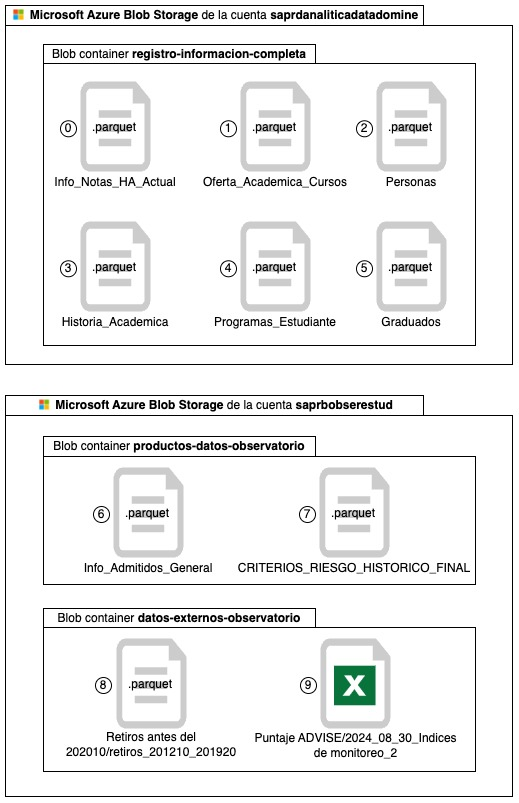
\includegraphics[width=0.7\textwidth]{assets/blob_storage.jpg}
	\caption{Archivos fuente y estructura de directorios en \gls{Azure Blob Storage}}
	\label{fig:blob_storage}
\end{figure}

Cada uno de los archivos presentados en la figura \ref{fig:blob_storage} se carga en el cuaderno de \gls{Jupyter} y se extrae la información relevante para el Perfil del estudiante. La tabla \ref{tab:extraccion} detalla el orden en el que se realiza cada extracción, describe la información que se extrae y especifica el archivo fuente del cual se obtiene, empleando la numeración de los archivos definida en la figura \ref{fig:blob_storage}.

\begin{longtblr}[
		caption = {Extracción de datos},
		label = {tab:extraccion_datos},
	]{
		colspec = {X[1,l] X[2,l] X[4,l] X[2,l]},
	}
	\hline
	\textbf{Orden} & \textbf{Información}                               & \textbf{Descripción}                                                                                                                 & \textbf{Archivos fuente} \\
	\hline
	1              & Histórico académico                                & Información de las notas obtenidas por los estudiantes en cada una de las asignaturas que han cursado.                               & 0                        \\
	2              & Oferta \newline académica                          & Información de las asignaturas que se ofertan en cada uno de los semestres académicos.                                               & 1                        \\
	3              & Estudiantes                                        & Información básica de los estudiantes.                                                                                               & 2, 3, 6                  \\
	4              & Programas académicos                               & Información de los programas académicos en los que se encuentran inscritos los estudiantes.                                          & 4                        \\
	5              & Información \newline adicional \newline de retiros & Información sobre los retiros de los estudiantes para periodos anteriores al 2019-20, que no se encuentra en el Histórico académico. & 8                        \\
	6              & Graduados                                          & Información de los estudiantes que se han graduado.                                                                                  & 5                        \\
	7              & Criterios \newline de riesgo                       & Información de los criterios de riesgo que se utilizan para identificar a los estudiantes en riesgo académico.                       & 7                        \\
	8              & Advise                                             & Información de los estudiantes tomada de la plataforma Advise.                                                                       & 9                        \\
	\hline
\end{longtblr}

\subsection{Transformación de los datos}

El proceso de transformación asegura que los datos extraídos sean consistentes, completos y relevantes para los análisis requeridos en el proyecto. Esto implica la aplicación de múltiples pasos destinados a mejorar la calidad de los datos y a garantizar su integridad, tanto desde una perspectiva técnica como desde el contexto académico de la Universidad.

A continuación, se mencionan solo algunos de los pasos más relevantes que se llevaron a cabo como parte del proceso de transformación. No se presenta el detalle de la implementación, que es extenso y no aporta valor al proyecto, pero se puede encontrar en el cuaderno de \gls{Jupyter} que implementa el \gls{pipeline} de analítica. Es importante señalar que la implementación del cuaderno debe cambiar conforme los datos en el Ecosistema evolucionen, su estructura cambie o su calidad mejore (o empeore).

\begin{itemize}
	\item \textbf{Variables a utilizar} Tras cargar los datos, existen una serie de variables que no son relevantes para el análisis y que se eliminan. Notablemente, se eliminan las cédulas de ciudadanía de los estudiantes, pues a partir de este punto se identifican mediante el código estudiantil. Otros ejemplos de variables descartadas son aquellas con información detallada de los acudientes del estudiante y con las especifidades de nacionalidades y direcciones de residencia.
	\item \textbf{Consistencia} Se evalúa la consistencia de los datos en pos de unificar tipos y formatos, eliminando inconsistencias y redundancias. Esto es particularmente importante, ya que, al provenir de archivos en formato PARQUET y XLSX, las columnas no poseen un tipo de dato intrínseco, lo que impide garantizar que los datos presuntamente numéricos en efecto lo sean. Ejemplos simples de esto son la transformación del código estudiantil y del periodo a tipos numéricos. Recuérdese que el periodo académico se representa con un número entero que concatena al año y el periodo académico, verbigracia, 201910 representa el primer semestre del año 2019, que convencionalmente se escribe como 2019-10.
	\item \textbf{Validez} Se verifica la validez de los datos. Por ejemplo, se descartan registros con valores nulos en campos críticos como el código estudiantil o el periodo académico, pues resulta inviable realizar un análisis académico sin información de estos campos.
	\item \textbf{Unicidad} Se garantiza la unicidad de los datos, mediante la eliminación de registros duplicados.
	\item \textbf{Completitud y relevancia} Se completan los datos faltantes, asignando valores predeterminados a campos críticos como la calificación final de materias. Se separan los datos que son irrelevantes para los cálculos académicos, como las materias relacionadas con deportes; no se eliminan, pues luego se reincorporan para ser mostrados como materias en el Perfil del estudiante.
	\item \textbf{Indicadores académicos} Se crean columnas adicionales y se calculan indicadores académicos relevantes que no existen en las fuentes originales de los datos. Algunos indicadores notables son:
	      \begin{itemize}
		      \item Se asignan clasificaciones a los estudiantes en estados como \textit{ACTIVO}, \textit{INACTIVO} o \textit{DESERTOR}, considerando el tiempo transcurrido desde su última matrícula.
		      \item Se realiza el cálculo de los créditos aprobados, reprobados, retirados, pendientes e incompletos, tanto de forma global como segmentada por áreas específicas como matemáticas, física y materias de la carrera.
		      \item Se calcula el número de matrículas del estudiante. Este indicador representa el número de semestres completos que han sido pagados y matriculados. Se calcula con dos decimales, donde un semestre completo equivale a una matrícula; media matrícula equivale a 0.5 matrículas; y un cuarto de matrícula, un periodo intersemestral, una práctica académica u otros casos similares equivalen a 0.25 matrículas. Esto provee una medida de la inversión realizada en la educación del estudiante mucho más precisa que simplemente el semestre en el que se encuentra matriculado.
	      \end{itemize}
\end{itemize}

Naturalmente, el proceso de transformación es mucho más extenso y detallado que lo presentado aquí. Estos ejemplos solo ilustran lo que ocurre en el proceso.

\subsection{Carga de los datos}

Tras el proceso de transformación, es necesario cargar los datos transformados en un sistema de almacenamiento que permita su consulta y análisis, no solo por parte del Perfil del estudiante, sino para otros análisis por parte de la Vicedecanatura de Asuntos Estudiantiles de la Facultad de Ingeniería o de cualquier otra dependencia de la Universidad.

A causa de eso, el notebook genera varios archivos PARQUET que almacenan la información transformada, organizándola semánticamente en archivos distintos para facilitar su consulta y análisis. Estos archivos se almacenan en el contenedor de Azure Blob Storage que se muestra en la figura \ref{fig:blobs_generados}.

\begin{figure}
	\centering
	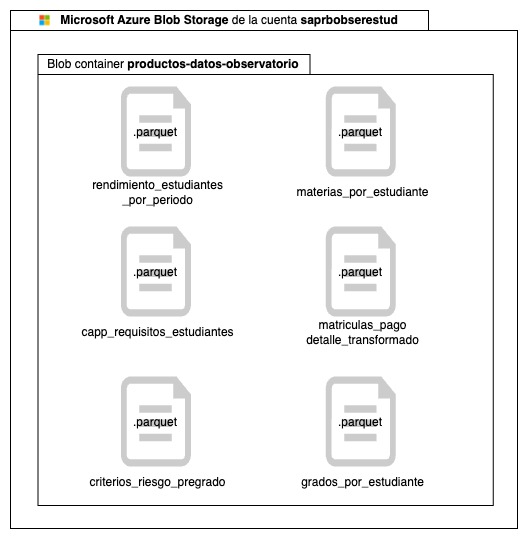
\includegraphics[width=0.7\textwidth]{assets/blobs_generados.jpg}
	\caption{Archivos generados por el proceso de transformación}
	\label{fig:blobs_generados}
\end{figure}

La tabla \ref{tab:blobs_generados} detalla los archivos generados y la información que contienen, a pesar de que los nombres de los archivos son autoexplicativos. En favor de la claridad, para cada archivo se describe de qué manera se debe interpretar cada registro. 

\begin{longtblr}[
		caption = {Archivos generados por el proceso de transformación y su contenido},
		label = {tab:blobs_generados},
	]{
		colspec = {X[1,l] X[3,l]},
	}
	\hline
	\textbf{Archivo}                        & \textbf{Contenido}                                                                                                  \\
	\hline
	rendimiento\_estudiantes\_por\_periodo  & Contiene el rendimiento académico de los estudiantes. Cada registro consta de indicadores académicos calculados para un estudiante en un periodo académico específico. \\
	criterios\_riesgo\_pregrado             & Almacena información relacionada con los criterios de riesgo académico en programas de pregrado. Cada registro corresponde a un estudiante e indica qué criterios de riesgo cumple, en caso de cumplir alguno. \\
	capp\_requisitos\_estudiantes           & Registra los requisitos cumplidos y pendientes de los estudiantes para la formalización de su grado. Cada registro representa un estudiante y especifica los requisitos cumplidos y los que aún están pendientes. \\
	materias\_por\_estudiante               & Incluye el detalle de las materias inscritas y su información correspondiente por estudiante y periodo académico. Cada registro representa un curso inscrito por un estudiante en un periodo académico. \\
	matriculas\_pago\_detalle\_transformado & Presenta las especificidades de las matrículas y los pagos realizados por los estudiantes tras la transformación de datos. Cada registro corresponde a un pago realizado por una fuente de financiación que cubre total o parcialmente la matrícula de un estudiante en un periodo académico. \\
	grados\_por\_estudiante                 & Contiene información sobre los grados obtenidos por los estudiantes, incluyendo fechas y programas. Cada registro corresponde a un grado obtenido por un estudiante. \\
	\hline
\end{longtblr}

Estos archivos se crean con el propósito de proporcionar la información que se almacena en la base de datos de \gls{PostgreSQL} del \gls{API REST}, que se describe en el capítulo \ref{ch:logica}. No obstante, su potencial de aplicación es considerablemente más amplio. Lamentablemente, los detalles del valioso uso que se les ha dado no pueden ser revelados en este documento.

\chapter{Capa de lógica}
\label{ch:logica}

Este capítulo se ocupa de describir la capa de lógica del sistema, comisionada con procesar los datos extraídos y exponerlos como recursos accesibles mediante una \gls{API REST}. Primeramente, inicia por justificar la construcción de un \gls{API REST} como interfaz de la capa de lógica. Posteriormente, se detalla el diseño del \gls{API}, describiendo la estructura de los datos y cómo se representan como objetos, en particular como clases, agnósticas de la fuente de los datos y de la implementación del \gls{API}. Tras eso, se dedican algunas secciones a la implementación del \gls{API}, abordando los aspectos técnicos relacionados con el desarrollo del \gls{API}, incluyendo el lenguaje de programación, el framework, la estructura de directorios de la implementación, así como las rutas y recursos expuestos por el \gls{API}. A eso le sigue una sección dedicada al despliegue del \gls{API}, tratando todos los detalles técnicos correspondientes. Finalmente, se dedica una sección a la calidad del código, detallando las herramientas y prácticas empleadas para garantizar la calidad del código.

\section{¿Por qué un API REST?}

Antes de entrar en detalles sobre el diseño del \gls{API}, es importante justificar la elección de un \gls{API REST} como interfaz de la capa de lógica del sistema. En primer lugar, un \gls{API REST} es una interfaz de programación de aplicaciones que sigue los principios del estilo arquitectónico \gls{REST}. Este estilo se basa en la transferencia de representaciones de recursos, que son identificados por \glslink{URI}{URIs}, y la manipulación de estos recursos mediante métodos estándar de \gls{HTTP}. En particular, un \gls{API REST} es una interfaz que facilita la interoperabilidad entre aplicaciones heterogéneas, permitiendo a un programa acceder a las funciones y datos de otro. En el caso de este proyecto, un \gls{API REST} es la interfaz ideal para exponer los datos procesados por la capa de lógica, ya que permite a cualquier aplicación, como el frontend del perfil del estudiante, acceder a estos datos de manera sencilla y eficiente.

En los últimos años, los \gls{API REST} han ganado popularidad en el desarrollo de aplicaciones web, ya que son fáciles de entender, escalables y flexibles. Además, un \gls{API REST} es independiente de la implementación subyacente, lo que significa que el frontend del perfil del estudiante no necesita conocer los detalles de cómo se procesan los datos o cómo se almacenan, sino que solo necesita conocer la interfaz del \gls{API}. Por último, un \gls{API REST} es fácil de probar y depurar, ya que se basa en estándares abiertos y bien conocidos, como \gls{HTTP} y \gls{JSON}.

En conjunto, estas características convierten al \gls{API REST} en la elección ideal para la capa de lógica de este sistema, ya que facilita exponer los datos procesados de manera sencilla y eficiente, independientemente de la implementación subyacente, y fácil de probar y depurar.

\section{Diseño del API}

El diseño del \gls{API} se divide en dos partes. La primera parte está en el marco de la programación orientada a objetos, y se encarga de describir cuál es la estructura de clases del \gls{API}: qué clases existen, cómo se relacionan entre sí y qué atributos tienen. La segunda parte se enfoca en la interfaz del \gls{API}, es decir, en cómo se exponen los datos procesados como recursos accesibles mediante una \gls{API REST}. Esto incluye los recursos expuestos, su representación, el formato en que se devuelven al cliente y los endpoints proporcionados por el \gls{API} para acceder a dichos recursos.

Cabe destacar que el diseño del \gls{API} es completamente independiente de dos factores: por un lado, la fuente de los datos, es decir, cómo se extraen de las fuentes originales; por otro, la implementación del \gls{API}, incluyendo el lenguaje y el framework utilizados para su desarrollo. En este sentido, esta sección es independiente del capítulo anterior, que estudia la capa de datos, y de la sección siguiente, que explica la implementación del \gls{API}.

\subsection{Estructura de clases del API}

Para modelar la información del Perfil del estudiante como objetos se optó por realizar un diagrama de clases conforme al estándar \gls{UML}. Esto presenta dos ventajas: por un lado, permite visualizar de manera clara y concisa la estructura de clases del \gls{API}. Por otro lado, es un artefacto bien conocido y ampliamente utilizado en el desarrollo de software, que no resultará ajeno a cualquier desarrollador que deba trabajar con el \gls{API} en el futuro.

\subsubsection{Diagrama de clases}

Se realizaron varias iteraciones en la construcción del diagrama de clases, teniendo en cuenta las necesidades del \gls{frontend} del perfil del estudiante y las restricciones de la capa de datos. La figura \ref{fig:diagrama_clases} muestra el diagrama de clases final del \gls{API}.

\begin{figure}[h]
	\centering
	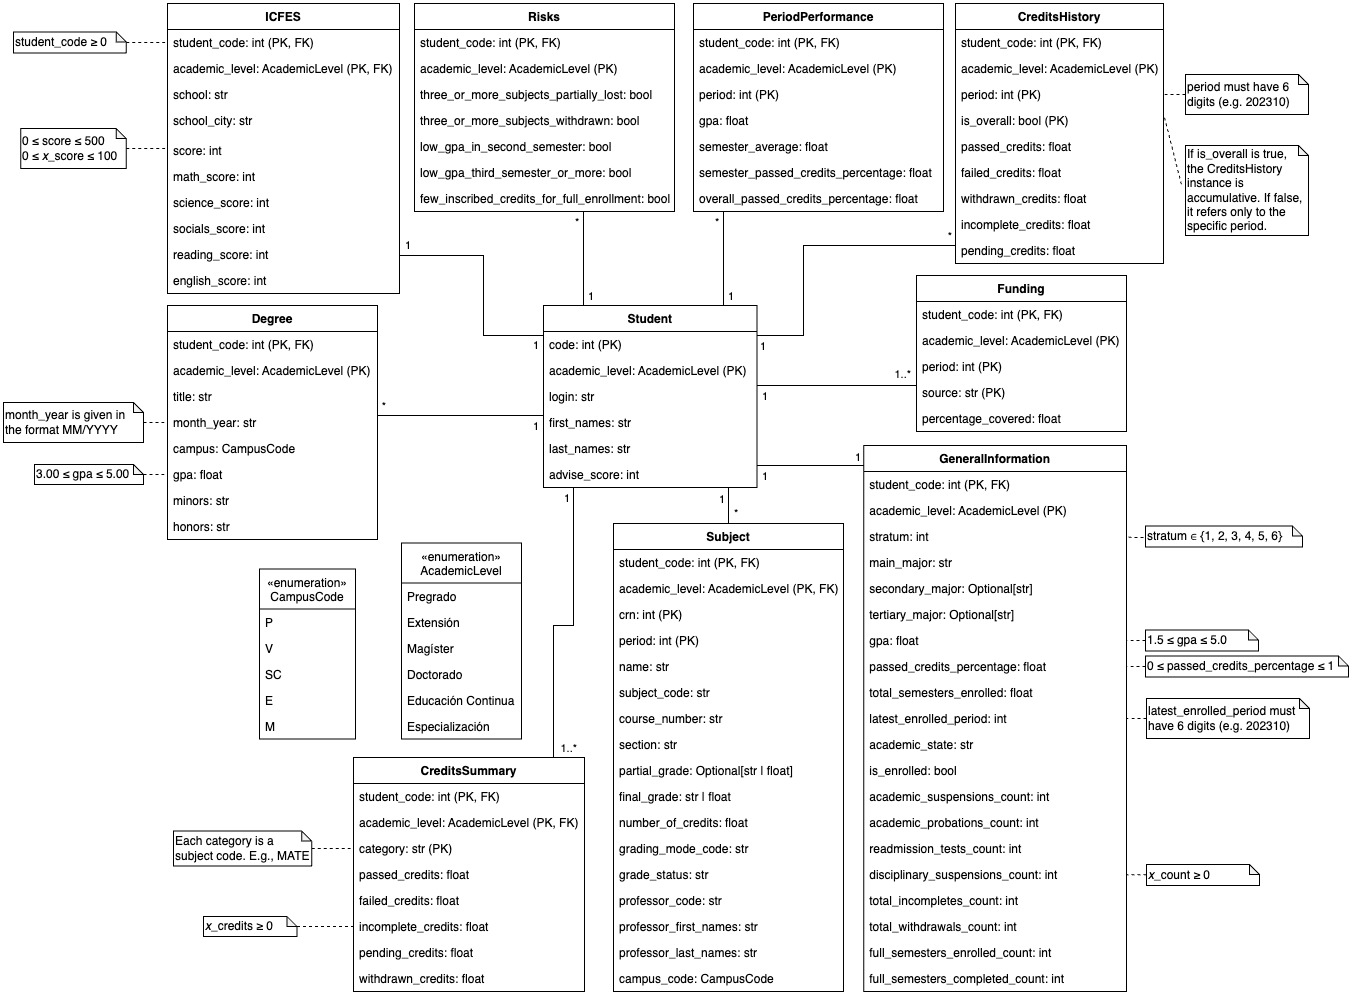
\includegraphics[width=\textwidth]{img/diagrama-clases.jpg}
	\caption{Diagrama de clases del \gls{API}}
	\label{fig:diagrama_clases}
\end{figure}

El diagrama de clases está escrito en inglés, siguiendo las convenciones de \gls{UML}. Cada clase tiene un nombre, que es un sustantivo en singular, y una serie de atributos. Los atributos están escritos en el formato \lstinline|nombre: tipo|, donde \lstinline|nombre| es el nombre del atributo y \lstinline|tipo| es el tipo de dato del atributo. Por conveniencia, los tipos de datos empleados son los mismos que se utilizan en el lenguaje de programación \gls{Python}, que es el lenguaje en el que se implementa el \gls{API}, pero bien podrían usarse los tipos de datos de cualquier otro lenguaje de programación orientado a objetos sin afectar semánticamente el diagrama de clases, por lo que mantiene su independencia de la implementación.

\subsubsection{Clases del API}

La estructura de clases del \gls{API} se basa en el principio de responsabilidad única, que establece que cada clase debe tener una sola responsabilidad y representar un solo concepto en el dominio del problema. Las clases propuestas en el diagrama se presentan alfabetizadas en la tabla \ref{tab:clases}, con su nombre original en inglés, la traducción al español y una breve descripción de su responsabilidad.

\begin{longtblr}[
		caption = {Clases del \gls{API} y sus responsabilidades},
		label = {tab:clases},
	]{
		colspec = {X[1,l] X[1,l] X[2,l]}
	}
	\hline
	\textbf{Nombre original} & \textbf{Nombre traducido}       & \textbf{Responsabilidad}                                                                                                                                                                                                                                                                                                \\
	\hline
	CreditsHistory           & Historial de créditos           & Rastrea el estado global de los créditos del estudiante, incluyendo: aprobados, reprobados, retirados, pendientes e incompletos, tanto para periodos específicos, por ejemplo un semestre particular, como en general y hasta la fecha.                                                                                 \\
	CreditsSummary           & Resumen de créditos             & Proporciona un desglose categórico de los créditos aprobados, reprobados, retirados, pendientes e incompletos, para una categoría específica de materias. Algunos ejemplos de categoría pueden ser: las materias de la carrera principal, las materias de matemáticas, las materias de física, entre otras.             \\
	Degree                   & Título                          & Almacena información sobre los títulos académicos obtenidos por el estudiante, como el nombre del título, el campus, el promedio y menciones especiales, como títulos con honores.                                                                                                                                      \\
	Funding                  & Financiamiento                  & Detalla las fuentes de financiamiento del estudiante, que pueden incluir becas y créditos educativos, con el porcentaje cubierto por cada fuente.                                                                                                                                                                       \\
	GeneralInformation       & Información general             & Contiene datos generales del estudiante, como su carrera principal, estrato, GPA actual, entre otros indicadores relevantes.                                                                                                                                                                                            \\
	ICFES                    & ICFES                           & Almacena los puntajes del estudiante en las áreas evaluadas por el examen ICFES, como matemáticas, lectura y ciencias.                                                                                                                                                                                                  \\
	PeriodPerformance        & Rendimiento por\newline periodo & Guarda información del desempeño académico del estudiante en un periodo específico, incluyendo el promedio del semestre y el porcentaje de créditos aprobados.                                                                                                                                                          \\
	Risks                    & Riesgos                         & Identifica indicadores de riesgo académico, como bajo GPA en los primeros semestres o retiro de múltiples materias.                                                                                                                                                                                                     \\
	Student                  & Estudiante                      & Representa a un estudiante de la universidad cuando se encontraba en un nivel académico específico. Almacena la información esencial para la identificación del estudiante, como nombres, apellidos, código y usuario (\lstinline|login|, que corresponde al nombre de usuario en el correo electrónico institucional). \\
	Subject                  & Materia                         & Representa una materia específica cursada por el estudiante, incluyendo el nombre, el código, los créditos, el profesor, la nota obtenida y el estado de la materia.                                                                                                                                                    \\
	\hline
\end{longtblr}

Como complemento del diagrama de clases y de la tabla \ref{tab:clases}, vale la pena ahondar en algunas de las decisiones de diseño que se tomaron en la creación de las clases con base en el dominio del negocio:
\begin{itemize}
	\item La clase \lstinline|Student| es la clase principal del modelo. Salta a la vista que no representa a un estudiante por completo, sino que representa a un estudiante en un nivel académico específico. Esto se debe a que resulta conveniente tratar de forma distinta al mismo estudiante en diferentes niveles académicos, ya que su contexto puede haber cambiado significativamente: el título al que aspira es distinto, las materias que cursa son distintas, su desempeño académico puede haber mejorado o empeorado, e incluso su situación socioeconómica puede haber cambiado. La misma persona en pregrado no puede ser tratada de la misma forma que en posgrado.
	\item La clase \lstinline|CreditsSummary| es auxiliar y proporciona un desglose categórico de los créditos aprobados, reprobados, retirados, pendientes e incompletos, para una categoría específica de materias. Naturalmente, no para todos los estudiantes se incluyen las mismas categorías. Es decir, para un estudiante de ingeniería, Categorías relevantes pueden ser las materias Específicas de su rama del ingeniería, las materias de matemática y las materias de física. Sin embargo, para un estudiante de arte, incluso si el estudiante ha optado por cursar materias de matemática y física, esas categorías pueden no ser relevantes para su desempeño académico. Esto es un matiz que es difícil representar en un diagrama de clases, pues corresponde a especificidades del dominio del problema, por lo cual se aclara en este apartado.
	\item Puede que el lector se haya percatado que la clase \lstinline|Risks| está nombrada con un sustantivo en plural, lo cual aparentemente transgrede las convenciones de construcción de diagramas de clase. Eso no es un error, sino una decisión consciente de diseño. Se debe a que la clase \lstinline|Risks| no representa un riesgo académico en particular, sino que cada instancia de la clase corresponde a un conjunto de riesgos académicos, entre ellos bajo GPA y retiro de múltiples materias. Por lo tanto, el nombre en plural es más adecuado que el nombre en singular para representar la naturaleza de la clase.
\end{itemize}

\subsubsection{Relaciones entre las clases}

Las relaciones entre las clases se representan mediante líneas que unen las clases. Las relaciones en este diagrama son muy simples, lo cual fue una elección deliberada en pos de la simplicidad y la claridad. Cada línea representa una asociación entre dos clases y en sus extremos cuenta con números que indican la multiplicidad de la asociación, es decir, cuántos objetos de una clase están asociados con cuántos objetos de la otra clase. Un asterisco indica que hay muchos objetos asociados, mientras que un número indica la cantidad exacta de objetos asociados.

Como ejemplo, considérese la asociación entre la clase \lstinline|Student| que representa a un estudiante y la clase \lstinline|Degree| que representa un grado. Un estudiante puede estar asociado con algún grado, en caso de ya haberse graduado, con varios, en caso de haber obtenido varios grados, o con ninguno, en caso de no haberse graduado. Sin embargo, cada grado corresponde unívocamente a un estudiante. Por ende, la asociación entre la clase \lstinline|Student| y la clase \lstinline|Degree| es de uno a muchos, representada por la línea que une ambas clases con un 1 en el extremo de la clase \lstinline|Student| y un asterisco en el extremo de la clase \lstinline|Degree|.

La tabla \ref{tab:relaciones} detalla las relaciones entre las clases del diagrama de clases, con una breve descripción de la relación y la multiplicidad de la asociación. Se organizan en orden de aparición, de arriba a abajo y de izquierda a derecha, en el diagrama de clases.


\begin{longtblr}[
		caption = {Relaciones entre las clases del diagrama de clases},
		label = {tab:relaciones},
	]{
		colspec = {X[1,l] X[2,l] X[3,l]}
	}

	\hline
	\textbf{Clase 1}    & \textbf{Clase 2}               & \textbf{Descripción y Multiplicidad}                                                                                                                         \\  \hline
	\lstinline|Student| & \lstinline|GeneralInformation| & Un estudiante está asociado con una única instancia de información general. Multiplicidad: 1 a 1.                                                            \\
	\lstinline|Student| & \lstinline|ICFES|              & Un estudiante puede tener una única instancia de resultados del ICFES. Multiplicidad: 1 a 1.                                                                 \\
	\lstinline|Student| & \lstinline|Risks|              & Un estudiante tiene una única instancia de indicadores de riesgos académicos. Multiplicidad: 1 a 1.                                                          \\
	\lstinline|Student| & \lstinline|PeriodPerformance|  & Un estudiante puede estar asociado con muchos periodos de desempeño académico. Multiplicidad: 1 a muchos.                                                    \\
	\lstinline|Student| & \lstinline|CreditsHistory|     & Un estudiante puede tener muchos historiales de créditos, cada uno relacionado con un periodo específico o de manera acumulativa. Multiplicidad: 1 a muchos. \\
	\lstinline|Student| & \lstinline|CreditsSummary|     & Un estudiante tiene un resumen de créditos categorizado. Multiplicidad: 1 a 1.                                                                               \\
	\lstinline|Student| & \lstinline|Subject|            & Un estudiante está asociado con muchas materias, pero cada materia pertenece a un único estudiante. Multiplicidad: 1 a muchos.                               \\
	\lstinline|Student| & \lstinline|Degrees|            & Un estudiante puede haber obtenido múltiples títulos. Multiplicidad: 1 a muchos.                                                                             \\
	\lstinline|Student| & \lstinline|Funding|            & Un estudiante puede tener múltiples fuentes de financiamiento. Multiplicidad: 1 a muchos.                                                                    \\
	\lstinline|Subject| & \lstinline|CreditsSummary|     & Cada materia está categorizada en un resumen de créditos. Multiplicidad: 1 a 1.
	\\
	\hline
\end{longtblr}

\subsubsection{Reglas de negocio en el diagrama de clases}

En el diagrama de clases se pueden evidenciar anotaciones en algunos atributos. Varias de estas anotaciones corresponden a restricciones de integridad que se deben cumplir en el modelo de datos, que en últimas representan reglas del dominio del problema. A esto, usualmente se le denomina \textit{reglas de negocio} y son restricciones que se deben cumplir en el modelo de datos para que reflejen la realidad de manera fiel.

La tabla \ref{tab:anotaciones} detalla las anotaciones en el diagrama de clases que tienen esa función, junto con su significado en términos del dominio del problema, es decir, en el contexto de la Universidad. Se organizan en orden de aparición en el diagrama de clases, de arriba a abajo y de izquierda a derecha.

\begin{longtblr}[
		caption = {Anotaciones del diagrama de clases y su significado},
		label = {tab:anotaciones},
	]{
		colspec = {X[1,l] X[2,l] X[2,l]},
	}
	\hline
	\textbf{Anotación}                                                           & \textbf{Significado}                                                                                                       & \textbf{Justificación}                                                                                                                                                                                                                                             \\
	\hline
	\texttt{student\_code \ensuremath{\geq} 0}                                   & El código del estudiante debe ser mayor o igual a 0                                                                        & El código del estudiante debe ser un entero positivo que identifica únicamente a cada estudiante. No se permiten códigos negativos.                                                                                                                                \\
	\texttt{0 \ensuremath{\leq} score \ensuremath{\leq} 500}                     & El puntaje del ICFES (formalmente, la prueba Saber 11) debe estar entre 0 y 500                                            & El puntaje máximo en la prueba Saber 11 es 500, y el mínimo es 0.                                                                                                                                                                                                  \\
	\texttt{0 \ensuremath{\leq} x\_score \ensuremath{\leq} 100}                  & Los puntajes de las áreas evaluadas por el ICFES deben estar entre 0 y 100                                                 & Los puntajes de las áreas evaluadas por el ICFES se normalizan a una escala de 0 a 100.                                                                                                                                                                            \\
	\texttt{month\_year is given in the format MM/YYYY}                          & La fecha de graduación, que se representa como un mes y un año, debe tener el formato MM/YYYY                              & La fecha de graduación se codifica en el formato de mes y año para garantizar consistencia en los registros.                                                                                                                                                       \\
	\texttt{3.00 \ensuremath{\leq} gpa \ensuremath{\leq} 5.0}                    & El GPA debe estar entre 3.0 y 5.0                                                                                          & En el sistema de la Universidad, el GPA mínimo para graduarse es 3.0 y el máximo posible es 5.0.                                                                                                                                                                   \\
	\texttt{Each category is a subject code. E.g., MATE}                         & Cada categoría de un Resumen de créditos es un código de materia. Por ejemplo, MATE representa las materias de matemáticas & Las categorías de un Resumen de créditos se representan con códigos de materia. Esta decisión de diseño se explica en detalle arriba, en la descripción de la clase \lstinline|CreditsSummary|.                                                                    \\
	\texttt{x\_credits \ensuremath{\geq} 0}                                      & Los créditos aprobados, reprobados, retirados, pendientes e incompletos deben ser mayores o iguales a 0                    & No tiene sentido registrar un número negativo de créditos en ningún contexto académico.                                                                                                                                                                            \\
	\texttt{period must have 6 digits (e.g. 202310)}                             & El periodo académico debe tener 6 dígitos                                                                                  & Los periodos académicos se codifican en el formato de año seguido por el indicador del tipo de periodo. Usualmente se usa un guión entre el año y el tipo de periodo, e.g., 2023-10, pero en este caso resulta más conveniente usar un número entero de 6 dígitos. \\
	\texttt{stratum \ensuremath{\in} \{1, 2, 3, 4, 5, 6\}}                       & El estrato socioeconómico debe estar entre 1 y 6                                                                           & Los estratos socioeconómicos en Colombia están normados en este rango por ley. Si el estudiante no reside en Colombia, no se registra su estrato.                                                                                                                  \\
	\texttt{1.5 \ensuremath{\leq} gpa \ensuremath{\leq} 5.0}                     & El GPA debe estar entre 1.5 y 5.0                                                                                          & En el sistema de la Universidad, el GPA mínimo posible es 1.5, y el máximo posible es 5.0.                                                                                                                                                                         \\
	\texttt{0 \ensuremath{\leq} passed\_credits\_percentage \ensuremath{\leq} 1} & El porcentaje de créditos aprobados debe estar entre 0 y 1                                                                 & Todo porcentaje es un número entre 0 y 1, inclusive.                                                                                                                                                                                                               \\
	\texttt{latest\_enrolled\_period must have 6 digits (e.g. 202310)}           & El periodo académico más reciente en el que el estudiante estuvo inscrito debe tener 6 dígitos                             & Esta explicación es análoga a la de la anotación \lstinline|period must have 6 digits (e.g. 202310)|.                                                                                                                                                              \\
	\hline
\end{longtblr}

\section{Implementación del API}

Esta sección se ocupa de la implementación del \gls{API REST}. En particular, se centra en los aspectos técnicos relacionados con el desarrollo del \gls{API}, incluyendo el lenguaje de programación, el framework y las herramientas asociadas a la implementación.

\subsection{Lenguaje y framework}

El \gls{API REST} está implementado en \gls{Python}, utilizando el framework \gls{FastAPI}. Se dedica un apartado a justificar la elección de cada uno de ellos.

\subsubsection{Python}

Un breve pero excelente resumen de las características del lenguaje se encuentra en la documentación oficial:
\begin{quote}
	\gls{Python} es un lenguaje interpretado, interactivo y orientado a objetos. Incorpora módulos, excepciones, tipado dinámico, tipos de datos dinámicos de muy alto nivel y clases. Además de la programación orientada a objetos, admite múltiples paradigmas de programación, como la programación procedural y funcional. \gls{Python} combina una potencia notable con una sintaxis muy clara. Ofrece interfaces a numerosas llamadas y bibliotecas del sistema, así como a distintos sistemas de ventanas, y es extensible en C o C++. También puede utilizarse como lenguaje de extensión para aplicaciones que requieran una interfaz programable. Finalmente, \gls{Python} es portátil: se ejecuta en diversas variantes de Unix, incluyendo Linux y macOS, así como en Windows. \cite{python_official_docs}
\end{quote} % TODO: Solve extra spacing issue
\noindent Existe una infinidad de argumentos técnicos para usar \gls{Python} en cualquier proyecto de software, que están bien documentadas en muchísimos recursos; por ejemplo, \cite{learning_python} tiene en su primer capítulo una sección dedicada exclusivamente a las razones por las cuales millones de desarrolladores alrededor del mundo usan el lenguaje. Por ende, no ahondaré en razones técnicas para elegir \gls{Python}.

No obstante, cabe mencionar una que existe una justificación contextual para elegir \gls{Python} para la implementación del \gls{API REST}, la cual es independiente de sus virtudes técnicas y responde a preocupaciones por la mantenibilidad del proyecto. En concreto, \gls{Python} es el principal lenguaje de programación que se enseña en la Universidad. Bajo la estructura curricular actual, en todos los programas de las facultades de Ingeniería, Ciencias y Economía, el curso ISIS-2021: Introducción a la Programación es obligatorio y constituye el primer curso de programación. % TODO: Cita!

Este curso, que \say{introduce conceptos básicos de programación, utilizados para resolver problemas con un programa de computadora} \cite{ip}, se enseña enteramente en \gls{Python}. El siguiente curso de programación, ISIS-1225: Estructuras de Datos y Algoritmos, que es obligatorio para los programas de Matemática e Ingeniería de Sistemas y Computación, también se enseña en \gls{Python}. % TODO: Cita!
Por lo tanto, la mayoría de los estudiantes de la Universidad que cursan programas del área de STEM tienen experiencia previa en \gls{Python} y varios no tienen experiencia en ningún otro lenguaje de programación. Esta restricción contextual implicó que la elección de \gls{Python} para la implementación del \gls{API REST} fue prácticamente obligatoria en aras de garantizar la sostenibilidad del proyecto a largo plazo.

\subsubsection{FastAPI}

\say{\gls{FastAPI} es un framework moderno, rápido (de alto rendimiento) y fácil de usar para construir \glslink{API}{APIs} con \gls{Python} basado en las anotaciones de tipo estándar de \gls{Python}} \cite{fastapi_docs}.

La principal justificación para la elección de \gls{FastAPI} va de la mano con la alta prioridad que se le ha dado a la mantenibilidad del proyecto. Se buscaba un framework que tuviera una curva de aprendizaje corta para desarrolladores familiarizados con \gls{Python}, que fuera fácil de mantener y extender, y que facilitara construir buena documentación. Sorprendentemente, \gls{FastAPI} cumple con todos estos requisitos, sin comprometer su rendimiento. De hecho, \gls{FastAPI} es uno de los frameworks más rápidos para construir \glslink{API}{APIs} con \gls{Python}, superando a otros frameworks populares como Flask y Django \cite{fastapi_benchmarks}.

Respecto a la facilidad de aprendizaje, la sintaxis \gls{FastAPI} está basada en las anotaciones de tipo estándar de \gls{Python}. Esto permite que para cualquier desarrollador que conozca \gls{Python}, sea sencillo aprender \gls{FastAPI}, pues no requiere aprender sintaxis adicional. \cite{fastapi_features}. Respecto a la mantenibilidad del framework, se destaca su integración con herramientas de validación de datos, como \gls{Pydantic}, que permite definir modelos de datos y validar automáticamente los datos entrantes. Esta funcionalidad facilita el mantenimiento del código en tanto que cualquier cambio en los modelos de datos se refleja inmediatamente en la validación de los datos entrantes \cite{fastapi_features}.

Por último, se destaca la integración con herramientas de documentación automática. \gls{FastAPI} genera automáticamente documentación interactiva de la \gls{API REST}, que se puede acceder a través de dos rutas: \verb|/docs| y \verb|/redoc|. La primera ruta genera una interfaz interactiva basada en \gls{Swagger}, mientras que la segunda ruta genera una interfaz interactiva basada en \gls{Redoc} \cite{fastapi_features}. Ambas interfaces permiten explorar los recursos del \gls{API REST}, probarlos y ver la documentación generada automáticamente, lo cual simplifica enormemente la tarea de mantener el \gls{API REST}, ya que cualquier cambio en el código se ve reflejado en la documentación.

Las razones anteriores hacen de \gls{FastAPI} una excelente elección para la implementación de cualquier \gls{API}, y más para este proyecto en particular, considerando las restricciones contextuales enunciadas en la sección anterior.

\subsection{Estructura de directorios}

\gls{FastAPI} es un framework no opinionado, es decir, que permite al desarrollador elegir cómo estructurar su proyecto. Esto significa que hay una infinidad de formas de estructurar un proyecto de \gls{FastAPI}. La siguiente fue la estructura de directorios elegida para este proyecto:
\begin{itemize}
	\item \lstinline|README.md|
	\item \lstinline|app.log|
	\item \lstinline|db/|
	\item \lstinline|.env|
	\item \lstinline|dev.log|
	\item \lstinline|requirements.txt|
	\item \lstinline|sonar-project.properties|
	\item \lstinline|src/|
	      \begin{itemize}
		      \item \lstinline|\_\_init\_\_.py|
		      \item \lstinline|main.py|
		      \item \lstinline|authentication/|
		      \item \lstinline|azure\_interface/|
		      \item \lstinline|config/|
		      \item \lstinline|constants/|
		      \item \lstinline|files/|
		      \item \lstinline|models/|
		      \item \lstinline|persist\_from\_blobs/|
		      \item \lstinline|routers/|
		      \item \lstinline|schemas/|
		      \item \lstinline|services/|
		      \item \lstinline|utils/|
	      \end{itemize}
	\item \lstinline|tests/|
\end{itemize}

Nótese que no se reflejan todos los archivos y directorios del proyecto, sino únicamente aquellos que son relevantes para la estructura de código del \gls{API REST}. La tabla \ref{tab:estructura_directorios} detalla la función de cada directorio y archivo en el directorio raíz del proyecto.

\begin{longtblr}[
		caption = {Estructura de archivos y directorios del proyecto},
		label = {tab:estructura_directorios},
	]{
		colspec = {X[1,l] X[3,l]},
	}
	\hline
	\textbf{Directorio/Archivo}                              & \textbf{Descripción}
	\\
	\hline
	\lstinline|README.md|                                    & Archivo con documentación fundamental del proyecto, en concreto una breve descripción e instrucciones de ejecución del proyecto en un ambiente local. Está escrito en \gls{Markdown}, que es un lenguaje de marcado ligero, es decir, que permite dar formato al texto de forma sencilla.                                                                                                                                                                                                                                    \\
	\lstinline|app.log|                                      & Archivo de registro (\textit{log}) generado automáticamente en el que se almacena información como errores, advertencias y notificaciones generadas durante la ejecución de la aplicación. El archivo \lstinline|app.log| corresponde al entorno de producción; en el entorno de desarrollo se genera el archivo \lstinline|dev.log|, cuyo propósito es análogo. Se ahonda en el uso de este archivo en la sección \ref{sec:despliegue_api}                                                                                  \\
	\lstinline|db/|                                          & Directorio que almacena scripts relacionados con respaldos y restauración de la base de datos, además de otros archivos necesarios para la gestión de datos persistentes.                                                                                                                                                                                                                                                                                                                                                    \\
	\lstinline|.env|                                         & Archivo de configuración que almacena variables de entorno. Estas variables permiten definir valores sensibles o específicos del entorno, como: credenciales, configuraciones de la base de datos, claves o modos de ejecución (desarrollo, pruebas y producción), sin incluirlos directamente en el código fuente. El archivo no se incluye en el control de versiones por contener información sensible, pero en el README se incluyen instrucciones para construirlo, mientras se cuente con las credenciales necesarias. \\
	\lstinline|sonar-project|\newline\lstinline|.properties| & Archivo de configuración para \gls{SonarQube}. El uso del archivo y de \gls{SonarQube} se explica en la sección \ref{sec:calidad_codigo}.                                                                                                                                                                                                                                                                                                                                                                                    \\
	\lstinline|src/|                                         & Directorio principal que contiene el código fuente del proyecto. Su nombre es una abreviación convencional para \textit{source}, que en inglés significa \textit{fuente}.                                                                                                                                                                                                                                                                                                                                                    \\
	\lstinline|tests/|                                       & Directorio que contiene las \gls{pruebas unitarias} del proyecto. Se ahonda en las \gls{pruebas unitarias} en la sección \ref{sec:calidad_codigo}.                                                                                                                                                                                                                                                                                                                                                                           \\
	\hline
\end{longtblr}

Como complemento a la tabla \ref{tab:estructura_directorios}, la tabla \ref{tab:estructura_directorios_src} especifica la función de cada directorio y archivo dentro del directorio \lstinline|src/|.

\begin{longtblr}[
		caption = {Estructura de archivos y directorios dentro de \lstinline|src/|},
		label = {tab:estructura_directorios_src},
	]{
		colspec = {X[1,l] X[3,l]},
	}
	\hline
	\textbf{Directorio/Archivo}     & \textbf{Descripción}
	\\
	\hline
	\lstinline|__init__.py|         & Archivo vacío cuyo nombre indica que el directorio es un paquete en \gls{Python}.                                                                                                                                                                               \\
	\lstinline|main.py|             & Punto de entrada de la aplicación. Contiene la configuración del objeto \lstinline|FastAPI|, que es la instancia principal de la aplicación, la importación e inicialización de las rutas y la configuración de los \textit{\glslink{middleware}{middlewares}}. \\
	\lstinline|authentication/|     & Módulo que gestiona la autenticación y autorización de usuarios en el proyecto.                                                                                                                                                                                 \\
	\lstinline|azure_interface/|    & Módulo que contiene la lógica para interactuar con servicios de Azure.                                                                                                                                                                                          \\
	\lstinline|config/|             & Módulo que almacena configuraciones del proyecto y de su interacción con la base de datos.                                                                                                                                                                      \\
	\lstinline|constants/|          & Módulo que define constantes compartidas utilizadas en el proyecto.                                                                                                                                                                                             \\
	\lstinline|files/|              & Directorio que almacena archivos estáticos o temporales necesarios para el proyecto.                                                                                                                                                                            \\
	\lstinline|models/|             & Módulo en el que se definen las clases que representan las tablas de la base de datos, apalancándose de \gls{SQLAlchemy}, que actúa como \gls{ORM}.                                                                                                             \\
	\lstinline|persist_from_blobs/| & Módulo encargado de la persistencia de datos provenientes de \gls{BLOB}s o almacenamiento de objetos.                                                                                                                                                           \\
	\lstinline|routers/|            & Módulo que define las rutas del \gls{API REST}, organizando los puntos de entrada según su funcionalidad.                                                                                                                                                       \\
	\lstinline|schemas/|            & Módulo que define los esquemas de datos utilizados en el \gls{API REST}, como las estructuras para solicitudes y respuestas.                                                                                                                                    \\
	\lstinline|services/|           & Módulo que implementa las operaciones que es posible realizar sobre los recursos del API con base en la lógica de negocio del proyecto.                                                                                                                         \\
	\lstinline|utils/|              & Módulo que agrupa funciones auxiliares utilizadas en diferentes partes del proyecto.                                                                                                                                                                            \\
	\hline
\end{longtblr}

Vale la pena ahondar en cuatro de los directorios mencionados arriba, que constituyen el esqueleto de cualquier \gls{API}: \lstinline|models|, que representa el modelo de datos del \gls{API}; \lstinline|schemas|, que define los esquemas de datos utilizados en las solicitudes y respuestas del \gls{API}; \lstinline|services|, que contiene la lógica de negocio del proyecto; y \lstinline|routers|, que define las rutas del \gls{API REST}. Se dedica un apartado a cada uno de ellos.

\subsubsection{Modelos de datos}

El módulo \lstinline|models| contiene las clases que representan las tablas de la base de datos. En particular, cada archivo de \gls{Python} en el directorio \lstinline|models| define una clase que abstrae la estructura de una de las tablas de la base de datos relacional. La mayoría de los atributos de la clase corresponden a las columnas de la tabla y algunos atributos especiales definen las relaciones entre las tablas y las restricciones de integridad. Por ejemplo, la clase \lstinline|Student| en el archivo \lstinline|models/student.py| plasma la tabla \lstinline|students| en la base de datos.

Esta abstracción, en la que el modelo de datos relacional se expresa como un modelo de objetos, es una tarea común en el desarrollo de software en lenguajes orientados a objetos y convencionalmente se realiza siguiendo el patrón \gls{ORM} (\textit{Object-Relational Mapper}). Dicho patrón permite representar objetos como tablas en una base de datos relacional y viceversa, a pesar de la diferencia en las estructuras orientada a objetos y relacional (problema conocido como \textit{impedancia de mapeo}, en inglés \textit{object-relational impedance mismatch}). En este proyecto, la librería \gls{SQLAlchemy} encapsula la lógica de mapeo objeto-relacional, permitiendo que las clases de \gls{Python} se mapeen directamente a tablas de la base de datos relacional. El lector puede ser familiar con otros \glslink{ORM}{ORMs}, como JPA (\textit{Java Persistence API}) en Java o \textit{Entity Framework} en C\#, que cumplen una función análoga.

\subsubsection{Esquemas de datos}
\label{subsec:schemas}

El módulo \lstinline|schemas| define las clases que corresponden a los esquemas de datos utilizados en las solicitudes y respuestas del \gls{API}. Estas clases están implementadas utilizando \gls{Pydantic}, una librería que provee validación de datos y la generación automática de documentación para los modelos. Todas las clases relacionadas a una entidad específica se definen en un solo archivo, de manera que en el archivo \lstinline|schemas/student.py| se definen las clases que representan los esquemas de datos de la entidad \lstinline|Student|.

En general, los esquemas de datos son una abstracción que permite definir la estructura de los datos que se envían y reciben en el \gls{API}, y que facilita la validación de los datos y la generación de documentación. Para lectores familiarizados con otros lenguajes o frameworks de desarrollo web, esta capa del \gls{API} es análoga a los \textit{serializers} de Django en \gls{Python}, los DTOs (\textit{Data Transfer Objects}) de Spring en Java, las clases de contratos en ASP.NET en C\# y las interfaces o tipos definidos en NestJS en TypeScript, por mencionar algunos ejemplos.

Cada esquema se compone de múltiples clases, cada una de las cuales refleja el propósito de la operación para la que se utiliza. Se escriben cinco clases, cada una con un sufijo que indica su propósito: la clase base (con sufijo \lstinline|Base|, de forma que para una entidad \lstinline|Entity| la clase base se llamaría \lstinline|EntityBase|), cuyo propósito es declarar todos los atributos comunes a todas las clases en pos de minimizar la duplicación de código; la clase para creación de datos (\lstinline|EntityCreate|), que consta de los atributos necesarios para crear un objeto; la clase para actualización de datos (\lstinline|EntityUpdate|), que contiene los atributos necesarios para actualizar un objeto; y la clase para lectura de datos (\lstinline|EntityResponse|), que consta de los atributos mínimos que se devuelven en la respuesta del \gls{API}. Algunos objetos tienen además otra clase de respuesta extendida, con prefijo \lstinline|ExtendedResponse|, que contiene atributos adicionales que no son necesarios en todas las respuestas, pero que pueden ser útiles en ciertos contextos. Cada clase contiene configuraciones adicionales que proporcionan ejemplos representativos de los datos, que se ven reflejados automáticamente en la documentación del \gls{API}.

Esta estructura modular y estándar para todos los esquemas de datos facilita la reutilización del código y mantiene la consistencia dentro del proyecto. Incluso si los atributos necesarios para crear una clase y los necesarios para actualizarla son los mismos, se definen en clases separadas para mantener la coherencia y facilitar la extensión en el futuro. Al mantener una separación tan definida entre las estructuras de datos utilizadas en las peticiones y respuestas del \gls{API}, y las utilizadas internamente (como los modelos de la base de datos), se facilita el mantenimiento del proyecto, se evitan dependencias innecesarias y se reduce el riesgo de \gls{sobreexposición}, es decir, de entregar más información de la necesaria en las respuestas del \gls{API}. Eso último es especialmente importante en un proyecto que maneja datos sensibles, como el presente.

\subsubsection{Lógica de negocio}

El módulo \lstinline|services| contiene las funciones que implementan la lógica de negocio del proyecto. Cada archivo en este módulo encapsula todas las operaciones relacionadas con una clase específica. Por ejemplo, el archivo \lstinline|services/student.py| contiene todas las operaciones que se pueden realizar sobre la entidad \lstinline|Student|.

Al interior de cada servicio existen, como mínimo, las funciones necesarias para realizar todas las operaciones \gls{CRUD} (crear, leer, actualizar y eliminar, del inglés \textit{Create, Read, Update, Delete}) sobre la entidad correspondiente, y en algunos casos, funciones adicionales que implementan operaciones más complejas. Cada operación se organiza claramente y se nombra con un prefijo que indica su responsabilidad: las funciones para creación (prefijadas con \lstinline|create|, de manera que para una entidad \lstinline|Entity| la función se llamaría \lstinline|create_entity|) reciben datos validados y los almacenan en la base de datos; las funciones para lectura (\lstinline|get_entity_by_id|, \lstinline|get_all_entities|) realizan consultas específicas o generales sobre los modelos; las funciones para actualización (\lstinline|update_entity|) modifican registros existentes; y las funciones para eliminación (\lstinline|delete_entity|) eliminan los registros de la base de datos de manera controlada. Esta estructura estándar asegura que las operaciones básicas son consistentes en todas las entidades.

En cada función, el servicio interactúa tanto con los modelos como con los esquemas de datos. Los esquemas de datos se utilizan para validar los argumentos que cada función recibe. Se mencionó en la subsección \ref{subsec:schemas} que en cada esquema de datos se definen clases para creación (\lstinline|Create|) y actualización (\lstinline|Update|); estas clases se utilizan para validar los datos que ingresan a las funciones de creación (\lstinline|create_entity|) y actualización (\lstinline|update_entity|) de los servicios, respectivamente. Por su parte, los modelos cumplen su función como abstracción de la base de datos ofreciendo una interfaz orientada a objetos para interactuar con las tablas, permitiendo que cada función realice las operaciones correspondientes sobre los registros de la base de datos. Por ejemplo, la función \lstinline|create_student|, cuya responsabilidad es crear un estudiante, recibe un objeto de tipo \lstinline|CreateStudent|, cuya estructura es validada automáticamente por \gls{Pydantic}, y lo utiliza para crear una instancia del modelo \lstinline|Student|, que representa una nueva entrada en la tabla de estudiantes de la base de datos.

Durante el proceso de ejecutar la operación que le corresponde, cada función del servicio se encarga de verificar las reglas de negocio asociadas que son demasiado intricadas como para ser validadas por \gls{Pydantic}. Verbigracia, \gls{Pydantic} puede validar fácilmente que el periodo académico ingresado sea un número, pero no puede verificar que el periodo académico sea válido en el contexto de la Universidad; esta verificación corresponde a la lógica de negocio y se realiza en la función del servicio correspondiente. Varios ejemplos de estas reglas de negocio se mencionan en la tabla \ref{tab:anotaciones}.

En términos de analogía con otras tecnologías, el módulo \lstinline|services| es equivalente a las capas de servicio (\textit{service layers}) en frameworks como Spring en Java, los servicios en ASP.NET en C\#, y las clases de servicios en NestJS en TypeScript. Todos estos enfoques tienen como objetivo separar la lógica de negocio tanto de los objetos que representan los datos como de las rutas del API y las representaciones de los recursos.

\subsubsection{Rutas del API}
El módulo \lstinline|routers| define las rutas del \gls{API REST}, sirviendo como punto de entrada para las solicitudes \gls{HTTP} realizadas al sistema. Cada archivo en este módulo agrupa las rutas relacionadas con una entidad específica. Por ejemplo, el archivo \lstinline|routers/student.py| define las rutas bajo el prefijo \lstinline|/students|, donde cada ruta corresponde a una operación específica relacionada con la entidad \lstinline|Student|.

Cada ruta está asociada a una operación del \gls{API} cuya lógica está implementada en los servicios. Por ende, dependiendo del contenido del servicio, una ruta puede corresponder a una operación básica \gls{CRUD} o una operación personalizada que satisface necesidades específicas del negocio. Cada ruta está implementada como una función dentro del archivo y está decorada con un decorador de \gls{FastAPI} que indica el método \gls{HTTP} correspondiente. Los decoradores disponibles son \lstinline|@router.get|, \lstinline|@router.post|, \lstinline|@router.put| y \lstinline|@router.delete|, correspondientes a las operaciones estándar de \gls{HTTP}: \lstinline|GET|, \lstinline|POST|, \lstinline|PUT| y \lstinline|DELETE|.

Un aspecto clave del diseño es la interacción entre las rutas, los servicios (\lstinline|services|) y los esquemas (\lstinline|schemas|). Las funciones de los \textit{routers} actúan como intermediarias: reciben las solicitudes \gls{HTTP}, validan los datos de entrada utilizando esquemas (\lstinline|schemas|), delegan la lógica de negocio a las funciones correspondientes en los servicios y entregan respuestas estructuradas basadas en los esquemas de datos. Por ejemplo, una función que crea un estudiante utilizará un esquema \lstinline|StudentCreate| para validar los datos de entrada, invocará a la función \lstinline|create_student| del servicio que encapsula la creación del estudiante y entregará una respuesta estructurada utilizando el esquema \lstinline|StudentResponse| (o \lstinline|StudentExtendedResponse| si la ruta en cuestión requiere información adicional).

\sloppy
A causa del flujo anterior, los esquemas de tipo \lstinline|Response|, como \lstinline|StudentResponse|, desempeñan un papel fundamental en este proceso. Estos esquemas aseguran que las respuestas del \gls{API} estén estructuradas de manera consistente, incluyendo únicamente los atributos necesarios para el cliente y excluyendo información interna o sensible.
\fussy

Además de las operaciones \gls{CRUD}, los \textit{routers} incluyen validaciones adicionales para garantizar que las solicitudes sean válidas antes de delegar el procesamiento a los servicios. Estas validaciones pueden incluir la verificación de que los identificadores no sean nulos, que los datos ingresados sean válidos y que los recursos existan antes de realizar operaciones sobre ellos. Por ejemplo, una solicitud para eliminar un estudiante puede comprobar primero si el estudiante existe, averiguándolo a través del servicio, antes de llamar a la función de eliminación del servicio.

En términos de arquitectura, el módulo \lstinline|routers| es análogo a los controladores (\textit{controllers}) en frameworks como Spring en Java, ASP.NET en C\#, o NestJS en TypeScript. Al igual que en estas tecnologías, el propósito de los \textit{routers} es mantener la independencia entre la lógica de negocio y la lógica de la interfaz de usuario, de forma que los cambios en la lógica de negocio no afecten la interfaz de usuario y viceversa.

\section{Calidad de código}
\label{sec:calidad_codigo}

Teniendo en cuenta que el software producido es de alto valor para la universidad y, por ende, probablemente deberá ser mantenido, extendido y reutilizado en el futuro, su desarrollo fue sometido a rigurosos estándares de calidad de código. Esta sección detalla las herramientas y prácticas empleadas para garantizar la calidad del código.

\subsection{Análisis estático}

El código fuente del \gls{API} está escrito para que sea fácil de entender y mantener.

Se configuró \gls{SonarQube} para realizar análisis estático sobre el código, utilizando el \gls{perfil de calidad} estándar para \gls{Python} 3.11. Esta herramienta identifica posibles problemas en el código y genera métricas detalladas para el monitoreo continuo de la calidad. En particular, la herramienta se cerciora de que el código cumple con estándares mínimos de mantenibilidad, confiabilidad y seguridad.

La figura \ref{fig:sonarqube} presenta los resultados más recientes del análisis de \gls{SonarQube}.

\begin{figure}[H]
	\centering
	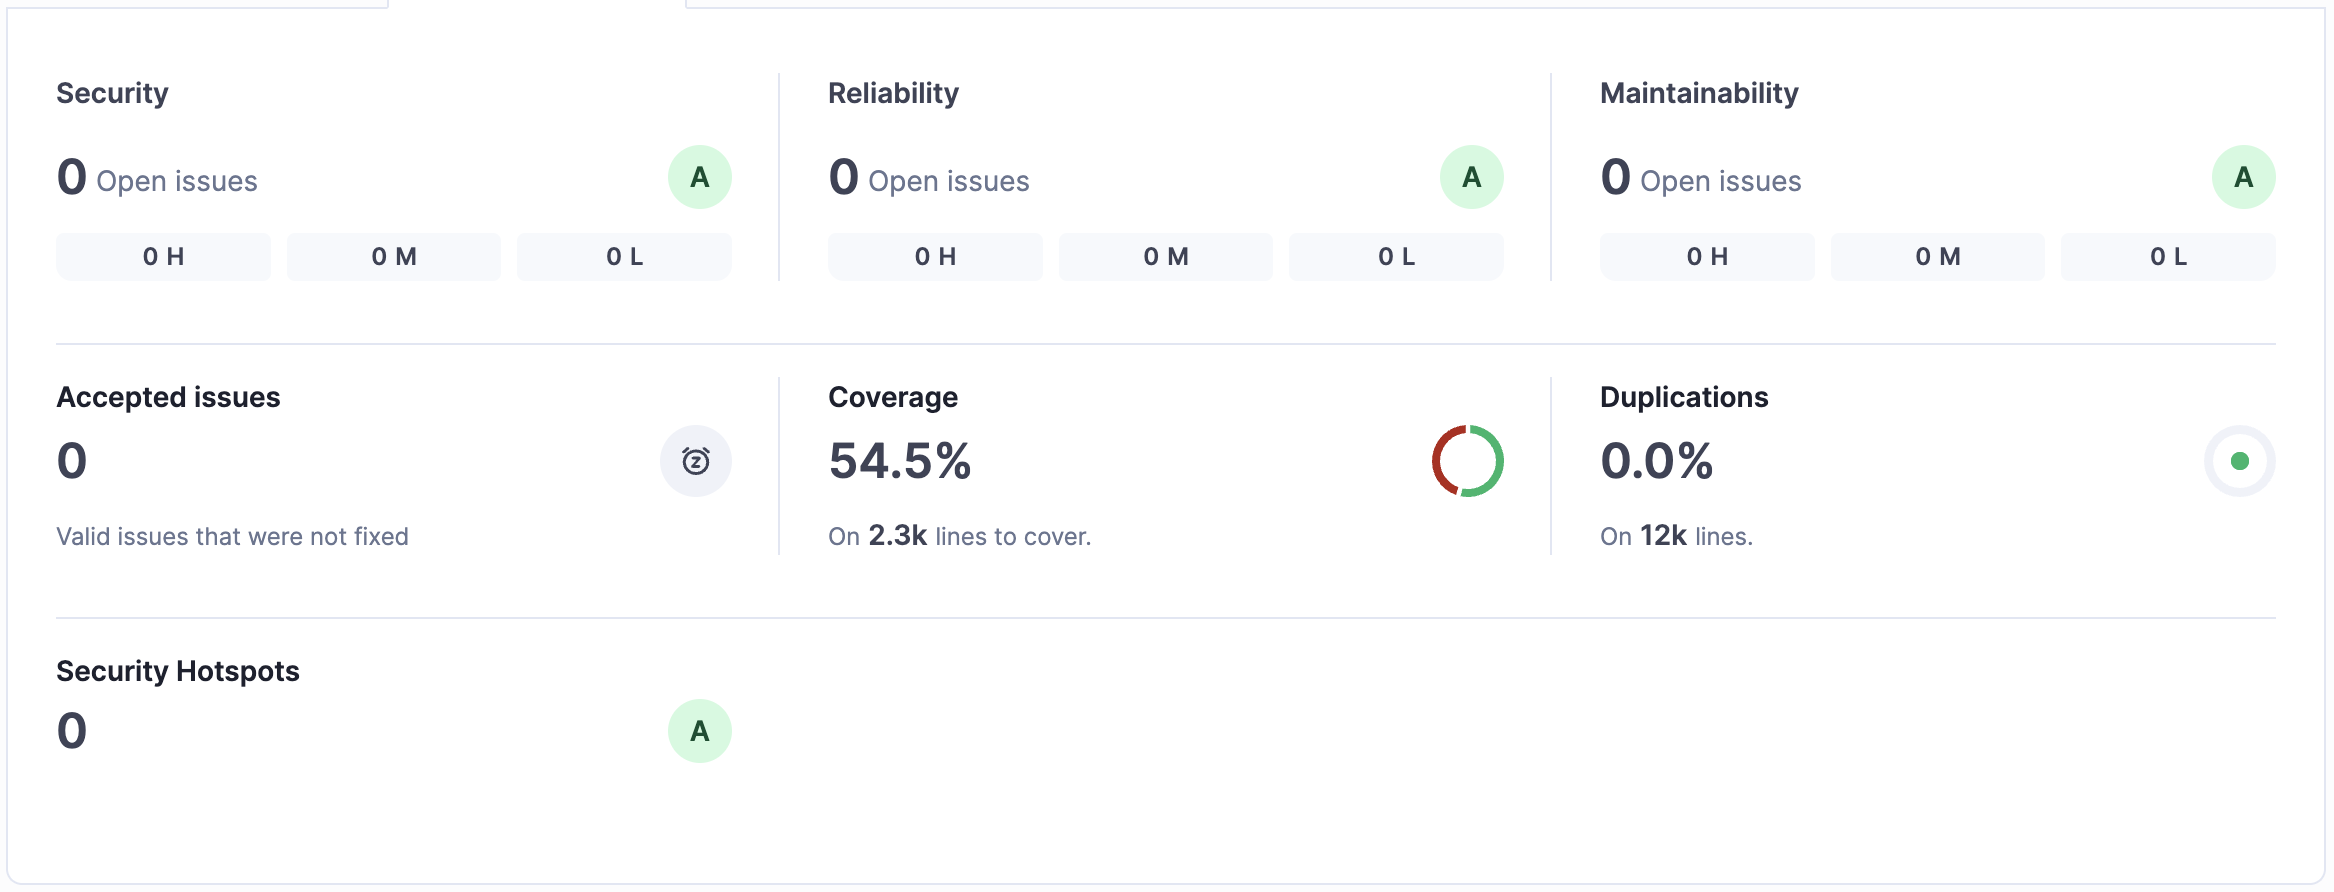
\includegraphics[width=\textwidth]{imagenes/sonarqube.png}
	\caption{Resultados del análisis de \gls{SonarQube}}
	\label{fig:sonarqube}
\end{figure}

Se evidencia que los resultados del análisis de \gls{SonarQube} son satisfactorios, con una calificación de A en todas las categorías, salvo en la cobertura de pruebas. Esto indica que el código cumple con los estándares de calidad definidos y que es altamente mantenible, confiable y seguro. Se reconoce que la cobertura de pruebas es una métrica que se debe mejorar en futuras iteraciones del proyecto. 

Más aún, en favor de garantizar un estilo de código uniforme y limpio, se emplearon las siguientes herramientas:
\begin{itemize}
	\item \gls{isort} y \gls{black} como \glslink{formateador}{formateadores} de código. El primero se encarga de ordenar las importaciones de los módulos de \gls{Python} de manera consistente, mientras que el segundo reformatea el código para asegurar un formato consistente. \glslink{black}{Black} garantiza que todos los proyectos de \gls{Python} que lo usan tengan el mismo estilo de código, lo que facilita la lectura y el mantenimiento del código a desarrolladores nuevos.
	\item \gls{Flake8} y \gls{SonarLint} como \glslink{linter}{linters}, para verificar la adherencia a las mejores prácticas y estándares de calidad de código. \gls{Flake8} es una herramienta de verificación de código que busca errores en el estilo del código \gls{Python}, mientras que \gls{SonarLint} es un \gls{linter} que se integra con \gls{SonarQube} y proporciona análisis en tiempo real del código.
\end{itemize}

\subsection{Documentación}

Existe extensa documentación del proyecto, tanto específica del API como general, incluyendo este documento. La documentación del \gls{API} se genera automáticamente a partir de los \glslink{docstring}{docstrings} de las funciones y métodos, gracias a las funcionalidades nativas de \gls{FastAPI} mencionadas arriba, y se puede acceder a través de las rutas \verb|/docs| y \verb|/redoc|.

Para que la documentación generada automáticamente resulte genuinamente útil, es indispensable que los parámetros utilizados por las funciones tengan nombres semánticamente correctos, que los tipos de datos sean explícitos y que todas las funciones estén debidamente documentadas. Para garantizar que ese sea el caso, se emplearon las prácticas descritas a continuación.

En primer lugar, para asegurar que los parámetros de las funciones estén bien nombrados y que los tipos de datos sean explícitos, resulta útil el uso de \gls{Pydantic} en la definición de los esquemas de datos. \gls{Pydantic} permite definir los tipos de datos de los atributos de las clases y automáticamente valida los datos que se le pasan a la clase. Por ejemplo, si se define una clase \lstinline|StudentCreate| con un atributo \lstinline|name| de tipo \lstinline|str|, \gls{Pydantic} se encargará de validar que el valor de \lstinline|name| sea una cadena de texto. Esto garantiza que los datos proporcionados a las funciones del \gls{API} sean válidos y que los desarrolladores que interactúen con el \gls{API} conozcan de antemano qué tipo de datos esperar.

En segundo lugar, respecto a la documentación de las funciones y métodos al interior del código, todas las funciones y métodos del \gls{API} están documentados mediante \glslink{docstring}{\textit{docstrings}}, siguiendo las convenciones definidas en el estándar \href{https://peps.python.org/pep-0257/}{\gls{PEP} 257}. Debido a que estas disposiciones son notablemente flexibles, se optó por la convención de \glslink{docstring}{docstrings} de \gls{NumPy}. Más específicamente, se satisfacen todos los lineamientos de la \href{https://python-sprints.github.io/pandas/guide/pandas_docstring.html}{guía de \glslink{docstring}{docstrings} de \gls{Pandas}}.

Para evitar omisiones, se emplea la librería \verb|flake8-docstrings| para verificar que los \glslink{docstring}{docstrings} sigan la convención de \gls{NumPy}. Esto se configura mediante la opción \verb|docstring-convention=numpy| en el archivo de configuración de \gls{Flake8}.

\subsection{Pruebas y automatización}

Sumado a lo anterior, se integraron diversas herramientas de automatización y pruebas para garantizar la calidad del código en cada modificación. En particular, se destacan las siguientes prácticas:

\begin{itemize}
	\item Se hizo uso de \gls{Pytest} para la creación y ejecución de \gls{pruebas unitarias}. \gls{Pytest} es una librería de pruebas que facilita la escritura y ejecución de pruebas en \gls{Python}. Se eligió \gls{Pytest} por su simplicidad y flexibilidad, que permiten escribir pruebas de manera clara y concisa.
	\item Se implementó un \gls{hook} de pre-commit de \gls{Git}, configurado para garantizar que el código está formateado y probado antes de cada \textit{commit}. El \gls{hook} de pre-commit se encarga de ejecutar \gls{isort}, \gls{black}, \gls{Flake8} y \gls{Pytest} antes de permitir que se realice un \textit{commit}. Si alguna de estas herramientas reporta un error, el \textit{commit} es rechazado y se notifica al desarrollador.
	\item Se dispone de un \gls{pipeline} en \gls{GitHub Actions} que ejecuta las pruebas, genera un reporte de cobertura y lo envía a \gls{SonarQube}. El \gls{pipeline} se ejecuta automáticamente cada vez que se realiza un \textit{push} a la rama principal del repositorio. Si alguna de las pruebas falla, el \gls{pipeline} se detiene y se notifica al desarrollador.
\end{itemize}

Estas prácticas aseguran que el código enviado a producción esté correctamente formateado, sea legible, esté probado y cumpla con los estándares de calidad establecidos.

\section{Infraestructura}

Esta sección describe la infraestructura utilizada para el despliegue del \gls{API} y la base de datos. La descripción se realiza a alto nivel y sin entrar en las características de la infraestructura, ya que estas son específicas de la Universidad y no son relevantes para el desarrollo del \gls{API}. Se hace hincapié en la elección de \gls{Docker} como tecnología de contenedores y en la separación de la base de datos en una máquina virtual aparte, por cuestiones de seguridad.

\subsection{Despliegue del API}
\label{sec:despliegue_api}

El despliegue del \gls{API} se realiza mediante el uso de contenedores \gls{Docker}, que permiten garantizar un entorno de ejecución uniforme y reproducible. Estos contenedores se alojan en una máquina virtual proporcionada por la universidad, la cual actúa como servidor central y asegura que el \gls{API} esté disponible de manera continua. La configuración del servidor garantiza que el contenedor de \gls{Docker} se mantenga siempre en ejecución, asegurando así la disponibilidad y la estabilidad del servicio.

El uso de \gls{Docker} ofrece múltiples beneficios. En primer lugar, permite simplificar el proceso de despliegue al encapsular todas las dependencias y configuraciones necesarias en el contenedor. Esto asegura que el \gls{API} se comporte de manera consistente en cualquier entorno, eliminando problemas derivados de diferencias en sistemas operativos o configuraciones locales. Además, facilita significativamente las actualizaciones y el mantenimiento. Cuando se realizan cambios en el \gls{API}, basta con hacer un \textit{pull} del repositorio en la máquina virtual y reiniciar el contenedor para que los cambios sean efectivos. Este enfoque minimiza tiempos de inactividad y reduce la posibilidad de errores humanos durante el proceso de despliegue. De hecho, se realizaron pruebas de modificación y despliegue y se determinó que el tiempo de indisponibilidad del servicio tras una actualización es inferior a 5 minutos.

\subsection{Base de datos}

La base de datos utilizada es \gls{PostgreSQL}, una solución robusta, escalable y ampliamente reconocida. \gls{PostgreSQL} ofrece características como soporte para transacciones ACID, manejo eficiente de consultas complejas y extensibilidad mediante módulos adicionales. Sumado a eso, es predominantemente la tecnología de bases de datos que se enseña en la Universidad, por lo cual se consideró una elección natural en favor de la continuidad del proyecto.

Por motivos de seguridad, la base de datos \gls{PostgreSQL} se encuentra alojada en una máquina virtual separada, accesible únicamente a través de la red interna Séneca de la universidad. Este diseño implementa una práctica conocida como \textit{air-gapping}, la cual consiste en aislar físicamente o lógicamente un sistema del acceso directo desde redes externas. En este caso, el \textit{air-gapping} asegura que la base de datos no pueda ser accedida desde dispositivos o redes externas a la Universidad, incluso si se dispone de las credenciales.

El uso del \textit{air-gapping} tiene particular sentido en este contexto, considerando la sensibilidad de la información gestionada. Los datos académicos y socioeconómicos del estudiantado están además protegidos por normativas de privacidad y protección de datos, lo cual propulsó la implementación de esta arquitectura.

\chapter{Capa de presentación}
\label{ch:presentacion}

El presente capítulo detalla el diseño y la implementación de la capa de presentación, cuya responsabilidad es proporcionar una interfaz de usuario intuitiva, interactiva, accesible y estéticamente consistente para el Perfil del estudiante.

Este es el capítulo más extenso y, probablemente, el más llamativo. Además de diversos aspectos técnicos correspondientes a la implementación del \gls{frontend}, exhibe y describe minuciosamente la interfaz del Perfil del estudiante, apoyándose en varias capturas de pantalla. Sin embargo, el lector debe tener presente que el desglose que aquí se realiza de la interfaz no suple la experiencia de navegación real en el Perfil del estudiante, directamente en la aplicación web \gls{NES}. Por tanto, se recomienda al lector que, en caso de tener acceso a la aplicación, explore el Perfil del estudiante directamente en ella.

El capítulo se ocupa primeramente de las cuestiones técnicas de la implementación de la capa de presentación, incluyendo el lenguaje y framework utilizados y la estructura de directorios del frontend. Tras eso, se describe, tan bien como es posible en un documento estático, la interfaz interactiva del Perfil del estudiante.

\section{Implementación del frontend}

\subsection{Lenguaje y framework}

El frontend está implementado en el framework \gls{React}, utilizando \gls{TypeScript} como lenguaje principal. El uso de React responde al hecho de que el resto de \gls{NES} está desarrollado bajo ese framework, por lo que se optó por mantener la consistencia con los demás módulos de la aplicación. Se descartó la implementación de microfrontends o alternativas similares puesto que se consideró que introducía complejidad adicional sin aportar beneficios significativos.

Por otro lado, se eligió \gls{TypeScript} por encima de \gls{JavaScript}, debido a que el tipado estático facilita la detección temprana de errores y mejora la mantenibilidad del código. Además, \gls{TypeScript} es un superset de \gls{JavaScript}, lo que garantiza su compatibilidad con el resto de módulos de la aplicación que se encuentran escritos en \gls{JavaScript}.

\subsection{Estructura de directorios del proyecto}

El frontend sigue una arquitectura modular, con el código al interior de la carpeta \lstinline|src| y cada página encapsulada en un directorio dentro de \lstinline|src/pages|. Esto favorece la organización del código y mejora su mantenibilidad. Dado que no compete a este trabajo detallar la estructura de directorios de NES en su totalidad, se describe solo superficialmente la estructura general del frontend, en la tabla \ref{tab:estructura_directorios_frontend}, a modo de contexto.

\begin{longtblr}[
		caption = {Estructura de directorios del proyecto},
		label = {tab:estructura_directorios_frontend},
	]{
		colspec = {X[1,l] X[3,l]}
	}
	\hline
	\textbf{Directorio/Archivo} & \textbf{Descripción}                                                                                                                                         \\
	\hline
	\lstinline|App.tsx|         & Componente principal de la aplicación, que sirve como punto de entrada y organiza las rutas.                                                                 \\
	\lstinline|Router.tsx|      & Configura las rutas de la aplicación, incluyendo la navegación al perfil del estudiante y a las otras páginas.                                               \\
	\lstinline|MainLayout.tsx|  & Componente que define el diseño general de la aplicación, incluyendo el encabezado, pie de página y disposición general.                                     \\
	\lstinline|pages/|          & Directorio que contiene el código asociado a cada página de la aplicación, como el perfil del estudiante.                                                    \\
	\lstinline|hooks/|          & Directorio que almacena hooks reutilizables en toda la aplicación, como manejo del estado global.                                                            \\
	\lstinline|components/|     & Contiene componentes reutilizables que se utilizan en varias páginas.                                                                                        \\
	\lstinline|constants/|      & Define constantes globales del proyecto, como configuraciones y estilos estándar.                                                                            \\
	\lstinline|services/|       & Implementa funciones para interactuar con otros servicios externos (distintos al \gls{API REST} del Perfil del estudiante) que alimentan el frontend.        \\
	\lstinline|assets/|         & Contiene recursos estáticos como imágenes utilizados en la aplicación.                                                                                       \\
	\lstinline|config/|         & Directorio con configuraciones específicas librerías como \gls{axios} y \gls{firebase}.                                                                      \\
	\lstinline|interfaces/|     & Define interfaces de \gls{TypeScript} que se utilizan para tipar datos y garantizar consistencia en el código.                                               \\
	\lstinline|recoilAtoms/|    & Contiene los \textit{atoms} de \gls{Recoil} para el manejo del estado global de la aplicación, que se utilizan para compartir información entre componentes. \\
	\lstinline|utils/|          & Agrupa funciones auxiliares reutilizables en diferentes partes del proyecto.                                                                                 \\
	\lstinline|index.css|       & Archivo principal de estilos CSS utilizado para definir configuraciones de diseño globales.                                                                  \\
	\hline
\end{longtblr}

El código correspondiente al Perfil del estudiante se encuentra en un solo directorio al interior de \lstinline|src/pages|, que es \lstinline|StudentProfilePage|. Naturalmente, en la implementación del Perfil del estudiante se importan y se reutilizan varias utilidades, interfaces, componentes y hooks de las carpetas \lstinline|src/utils|, \lstinline|src/iterfaces|, \lstinline|src/components| y \lstinline|src/hooks|, respectivamente, lo que asegura la consistencia y reduce la duplicación de código.

\subsubsection{Estructura del módulo del Perfil del estudiante}

\sloppy
El módulo del Perfil del estudiante está encapsulado en el directorio \lstinline|src/pages/StudentProfilePage|. Allí, el código a su vez está organizado en un subdirectorios por cada pestaña visual del Perfil del estudiante. Esta organización modulada facilita dos cosas:
\fussy

\begin{itemize}
	\item Realizar cambios de manera localizada, ya que cada pestaña es prácticamente un submódulo independiente.
	\item Asegurar que los permisos de usuario sean administrados correctamente, pues cada pestaña tiene diferentes niveles de acceso. Esto es especialmente importante para la pestaña Financiación, que contiene el detalle de la información financiera del estudiante y, por las políticas de gobierno de datos de la Universidad, solo debe ser accesible para directivos.
\end{itemize}

La estructura de directorios al interior del módulo del Perfil del estudiante se detalla en la tabla \ref{tab:estructura_modulo_perfil}.

\begin{longtblr}[
		caption = {Estructura de directorios del módulo del Perfil del estudiante},
		label = {tab:estructura_modulo_perfil},
	]{
		colspec = {X[2,l] X[3,l]}
	}
	\hline
	\textbf{Directorio/Archivo}       & \textbf{Descripción}                                                                                                 \\
	\hline
	\lstinline|performanceTab/|       & Contiene la pestaña de rendimiento académico.                                                                        \\
	\lstinline|fundingTab/|           & Contiene la pestaña de financiación.                                                                                 \\
	\lstinline|subjectsTab/|          & Contiene la pestaña con todas las materias inscritas por el estudiante.                                              \\
	\lstinline|scheduleTab/|          & Proporciona una vista del horario del estudiante.                                                                    \\
	\lstinline|personalDataCard/|     & Componente que muestra información personal del estudiante y se reutiliza en todas las pestañas.                     \\
	\lstinline|chips/|                & Contiene componentes específicos reutilizados únicamente dentro del perfil del estudiante, como botones y etiquetas. \\
	\lstinline|useStudentProfile.tsx| & Hook que centraliza la obtención de los datos del perfil desde el \gls{API REST}.                                    \\
	\hline
\end{longtblr}

Con respecto a la tabla anterior, cabe señalar que los componentes implementados en \lstinline|chips/| no se implementaron en la carpeta \lstinline|components/| del proyecto debido a que son específicos del Perfil del estudiante y no se reutilizan en otras partes de la aplicación. Dicho eso, en caso de que se requiera reutilizar estos componentes en otras partes de la aplicación, basta con moverlos a la carpeta \lstinline|components/| y ajustar las importaciones correspondientes.

Bajo un raciocinio similar, el hook \lstinline|useStudentProfile.tsx| se implementó dentro del directorio del módulo del Perfil del estudiante, en lugar de en \lstinline|hooks/|, porque se utiliza solamente en el Perfil del estudiante y no en otras partes de la aplicación. Es, además, el único código del frontend que se comunica con el \gls{API REST} del Perfil del estudiante, por lo que su ubicación en el módulo del Perfil del estudiante facilita la comprensión y el mantenimiento del código.

El \lstinline|hook| \lstinline|useStudentProfile.tsx| solicita toda la información relevante del \gls{API REST} del Perfil del estudiante en una única petición. Esto se hace así porque resulta más eficiente. Inicialmente, el diseño del \gls{API} contaba con un endpoint separado para cada recurso, lo que implicaba realizar múltiples peticiones independientes para cada pestaña. Sin embargo, se determinó que esta estructura incrementaba la latencia. Por esta razón, el \gls{API} fue rediseñado para agrupar todos los recursos en una única representación unificada, accesible mediante un solo endpoint.

\subsection{Ruta al perfil del estudiante}
\label{sec:ruta_perfil_estudiante}

Como ruta para acceder al perfil del estudiante desde \gls{NES} se seleccionó \lstinline|/perfil-estudiante/:correo|, donde \lstinline|:correo| corresponde al correo Uniandes, sin el dominio, del estudiante de quien se quiere ver el perfil. Por ejemplo, la ruta para acceder al perfil del autor de este documento es \lstinline|/perfil-estudiante/f.melo|.

Cualquier usuario que esté autenticado en \gls{NES} y cuente con los permisos adecuados, podrá acceder y visualizar directamente el perfil del estudiante al ingresar a la ruta indicada.

Esto facilita que los profesores y directivos de la Universidad puedan compartir perfiles de estudiantes de manera sencilla. En caso de que el lector tenga ese rol dentro de la Universidad, puede probar la funcionalidad iniciando sesión en \gls{NES} y luego pulsando en el siguiente enlace: \url{https://noestassolo.virtual.uniandes.edu.co/perfil-estudiante/f.melo}.

Se hace hincapié en que el usuario debe estar autenticado en \gls{NES} y debe contar con los permisos necesarios para acceder al perfil de un estudiante. De lo contrario, no podrá visualizarlo. En particular, ningún alumno podrá acceder al perfil de algún otro de esta manera (ni de ninguna otra, salvo que el otro pupilo o algún otro usuario autorizado deliberadamente se lo permita).

\section{Interfaz del Perfil del estudiante}

Esta sección describe la interfaz del Perfil del estudiante, mostrando capturas de pantalla de las diferentes pestañas y secciones que lo componen. Se describen las funcionalidades y la información presentada en cada una, junto con las decisiones de diseño adoptadas para garantizar claridad, relevancia y simplicidad.

Como se mencionó anteriormente, esta descripción no reemplaza la experiencia de navegación real en el Perfil del estudiante. Por tanto, se recomienda al lector que, en caso de tener acceso a la aplicación, explore el Perfil del estudiante directamente en ella.

Todas las capturas de pantalla en esta sección son reales. La gran mayoría corresponden al Perfil del estudiante del autor de este documento; aquellas que no, lo indican explícitamente, mencionando que corresponden a un estudiante anónimo en la descripción de la figura.

\subsection{Acceso al perfil del estudiante}

Los estudiantes, profesores y directivos de la Universidad cuentan con acceso al Perfil del estudiante, cada uno con diferentes niveles de permisos y restricciones de visualización. Los profesores y directivos pueden acceder a los perfiles de todos los estudiantes, mientras que los estudiantes únicamente pueden acceder a su propio perfil. Más aún, los directivos tienen acceso a la pestaña de Financiación, mientras que los profesores y estudiantes no tienen acceso a esta pestaña.

En la sección \ref{sec:ruta_perfil_estudiante} se explica una forma práctica de acceso al Perfil del estudiante mediante una URL específica. Sin embargo, la forma más común e intuitiva de acceso al Perfil del estudiante es desde la interfaz de \gls{NES}. El modo de acceso varía entre estudiantes, profesores y directivos, como se describe a continuación.

\subsubsection{Acceso al Perfil del estudiante como estudiante}

Cada alumno tiene la posibilidad de acceder a su propio Perfil del estudiante y tiene dos maneras de hacerlo. Para ambas, en primer lugar, debe iniciar sesión en \gls{NES} con su correo Uniandes y su contraseña, pulsando en el botón \textit{Iniciar sesión} en la esquina superior derecha de la página de inicio de \gls{NES}, que se muestra en la figura \ref{fig:landing}.

\begin{figure}[H]
	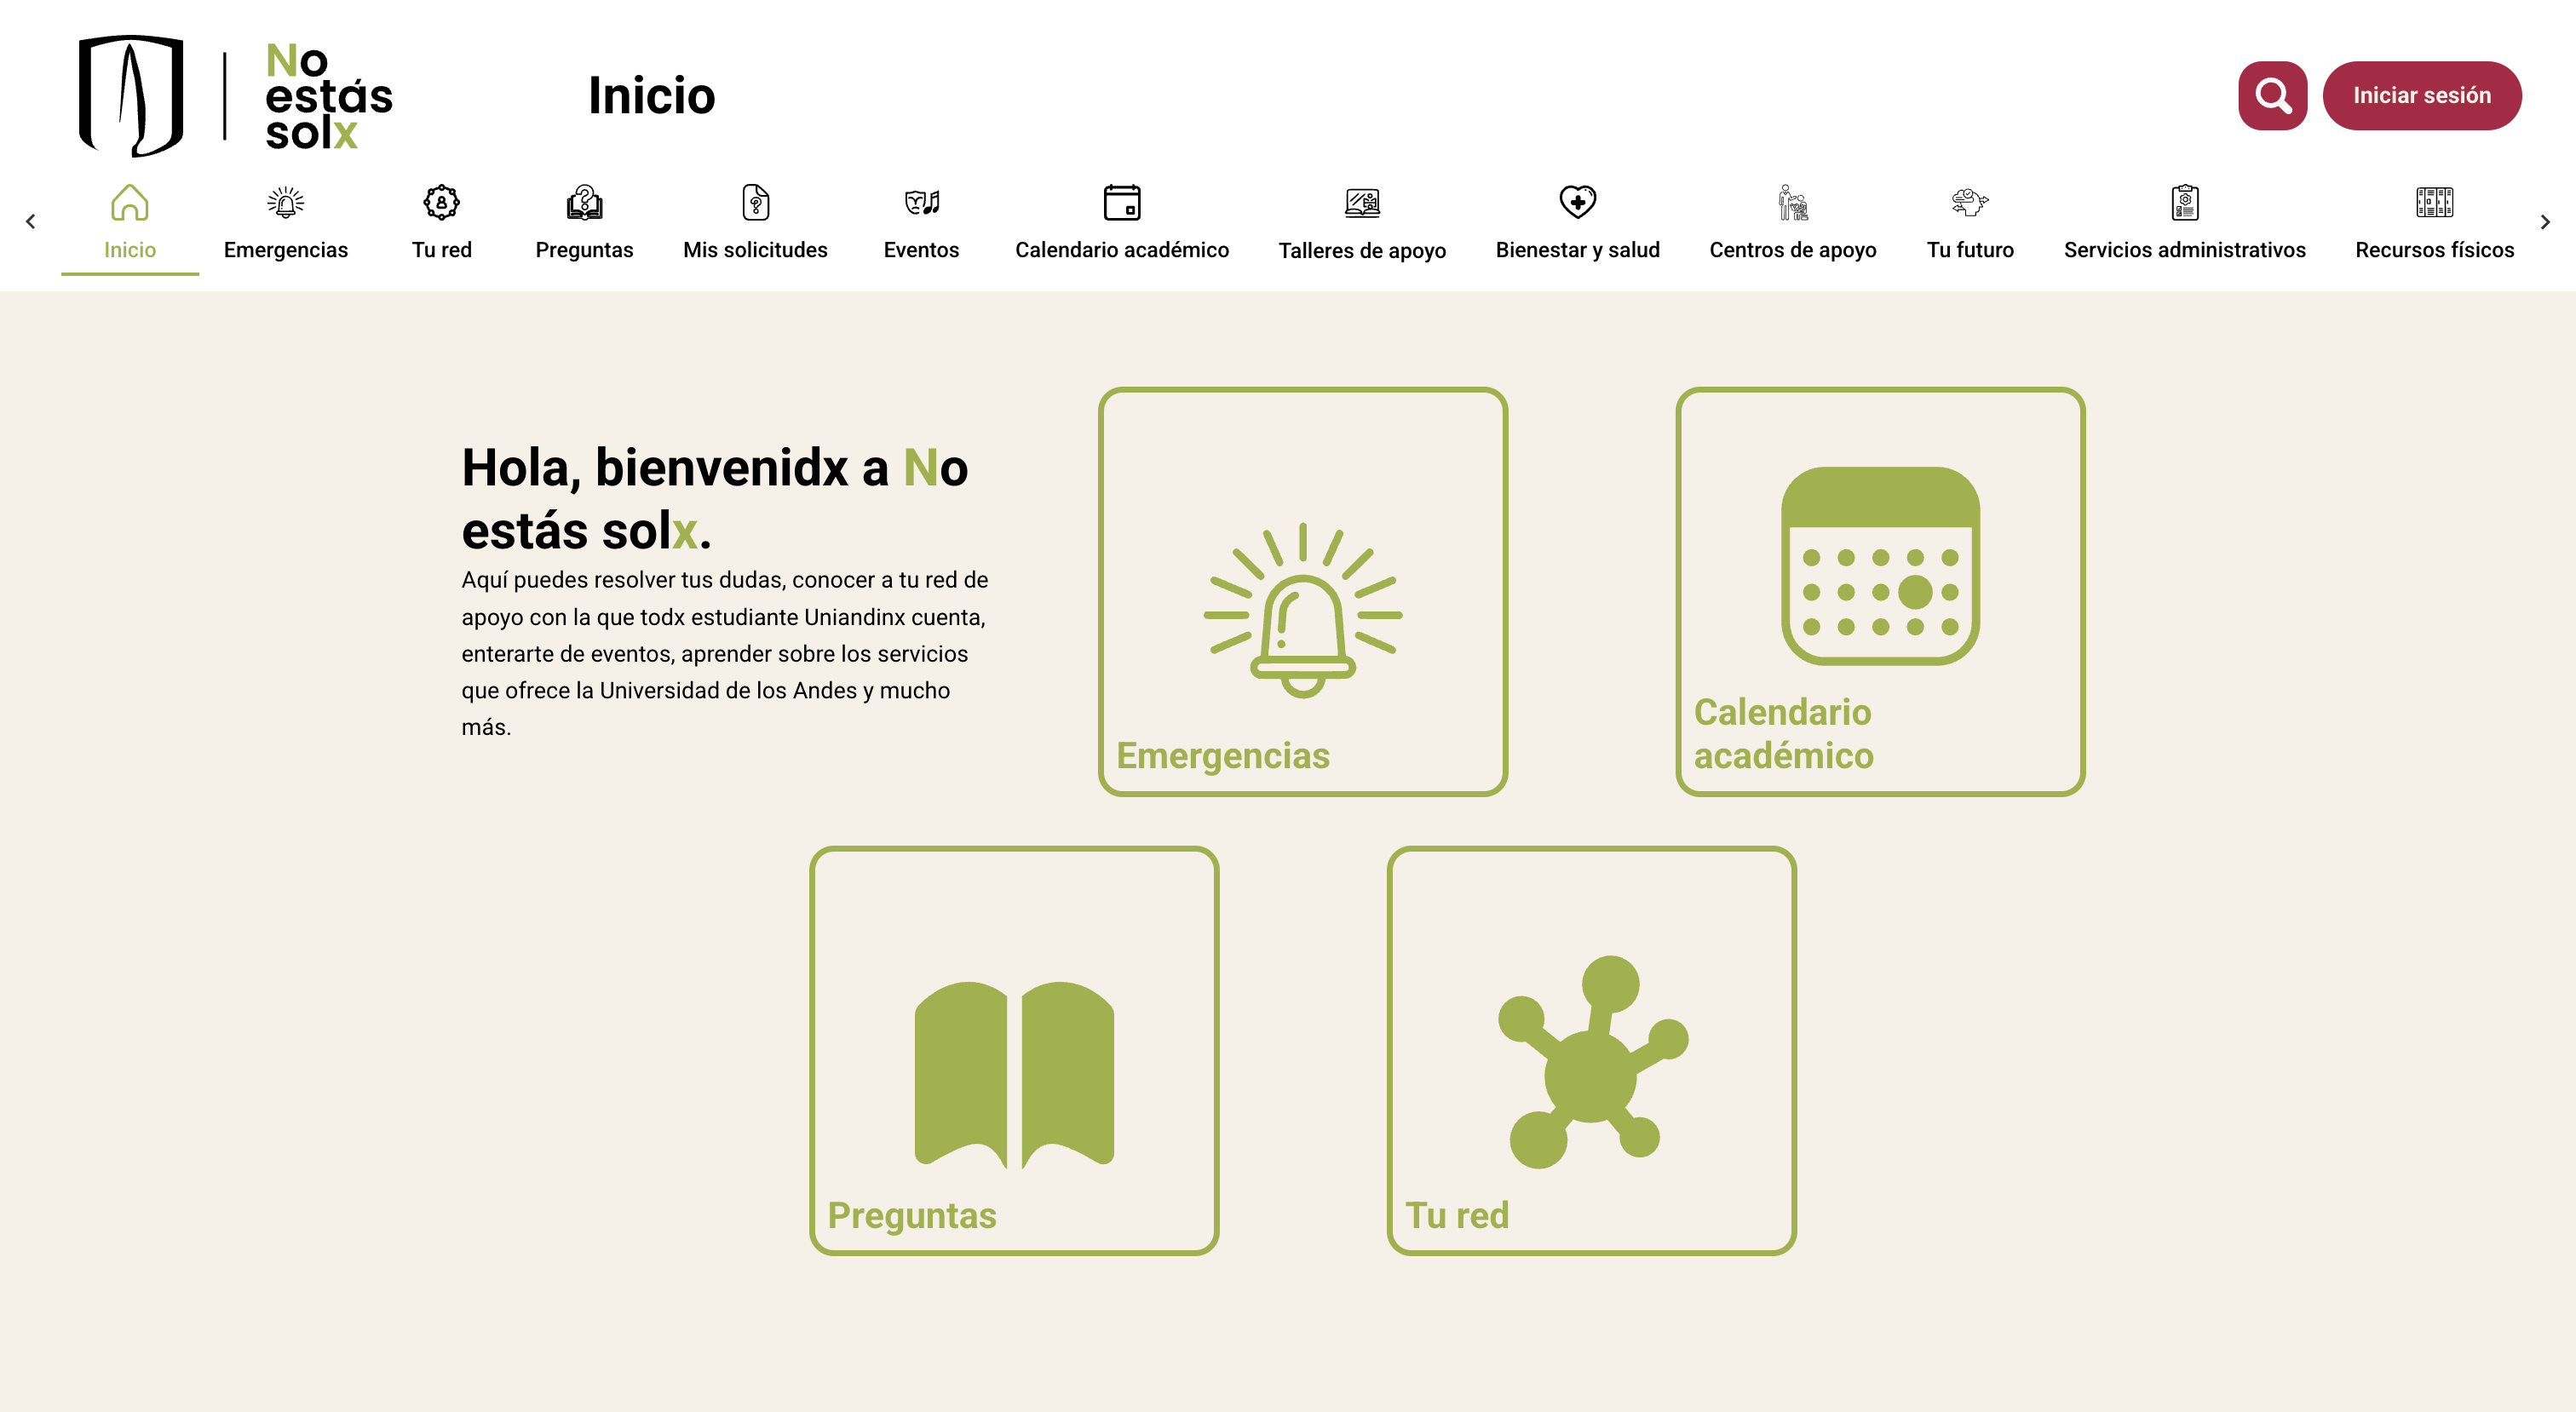
\includegraphics[width=\textwidth]{assets/nes/landing.png}
	\caption{Página inicial de NES.}
	\label{fig:landing}
\end{figure}

Una vez iniciada la sesión, la página inicial de NES se transforma a la vista de estudiante, como se muestra en la figura \ref{fig:landing_estudiante}. Esa vista difiere de la anterior en tanto que ahora existe un botón adicional, titulado Mi perfil académico. Esta es la primera forma de acceder al Perfil del estudiante: pulsando el botón \textit{Mi perfil académico}.

\begin{figure}[H]
	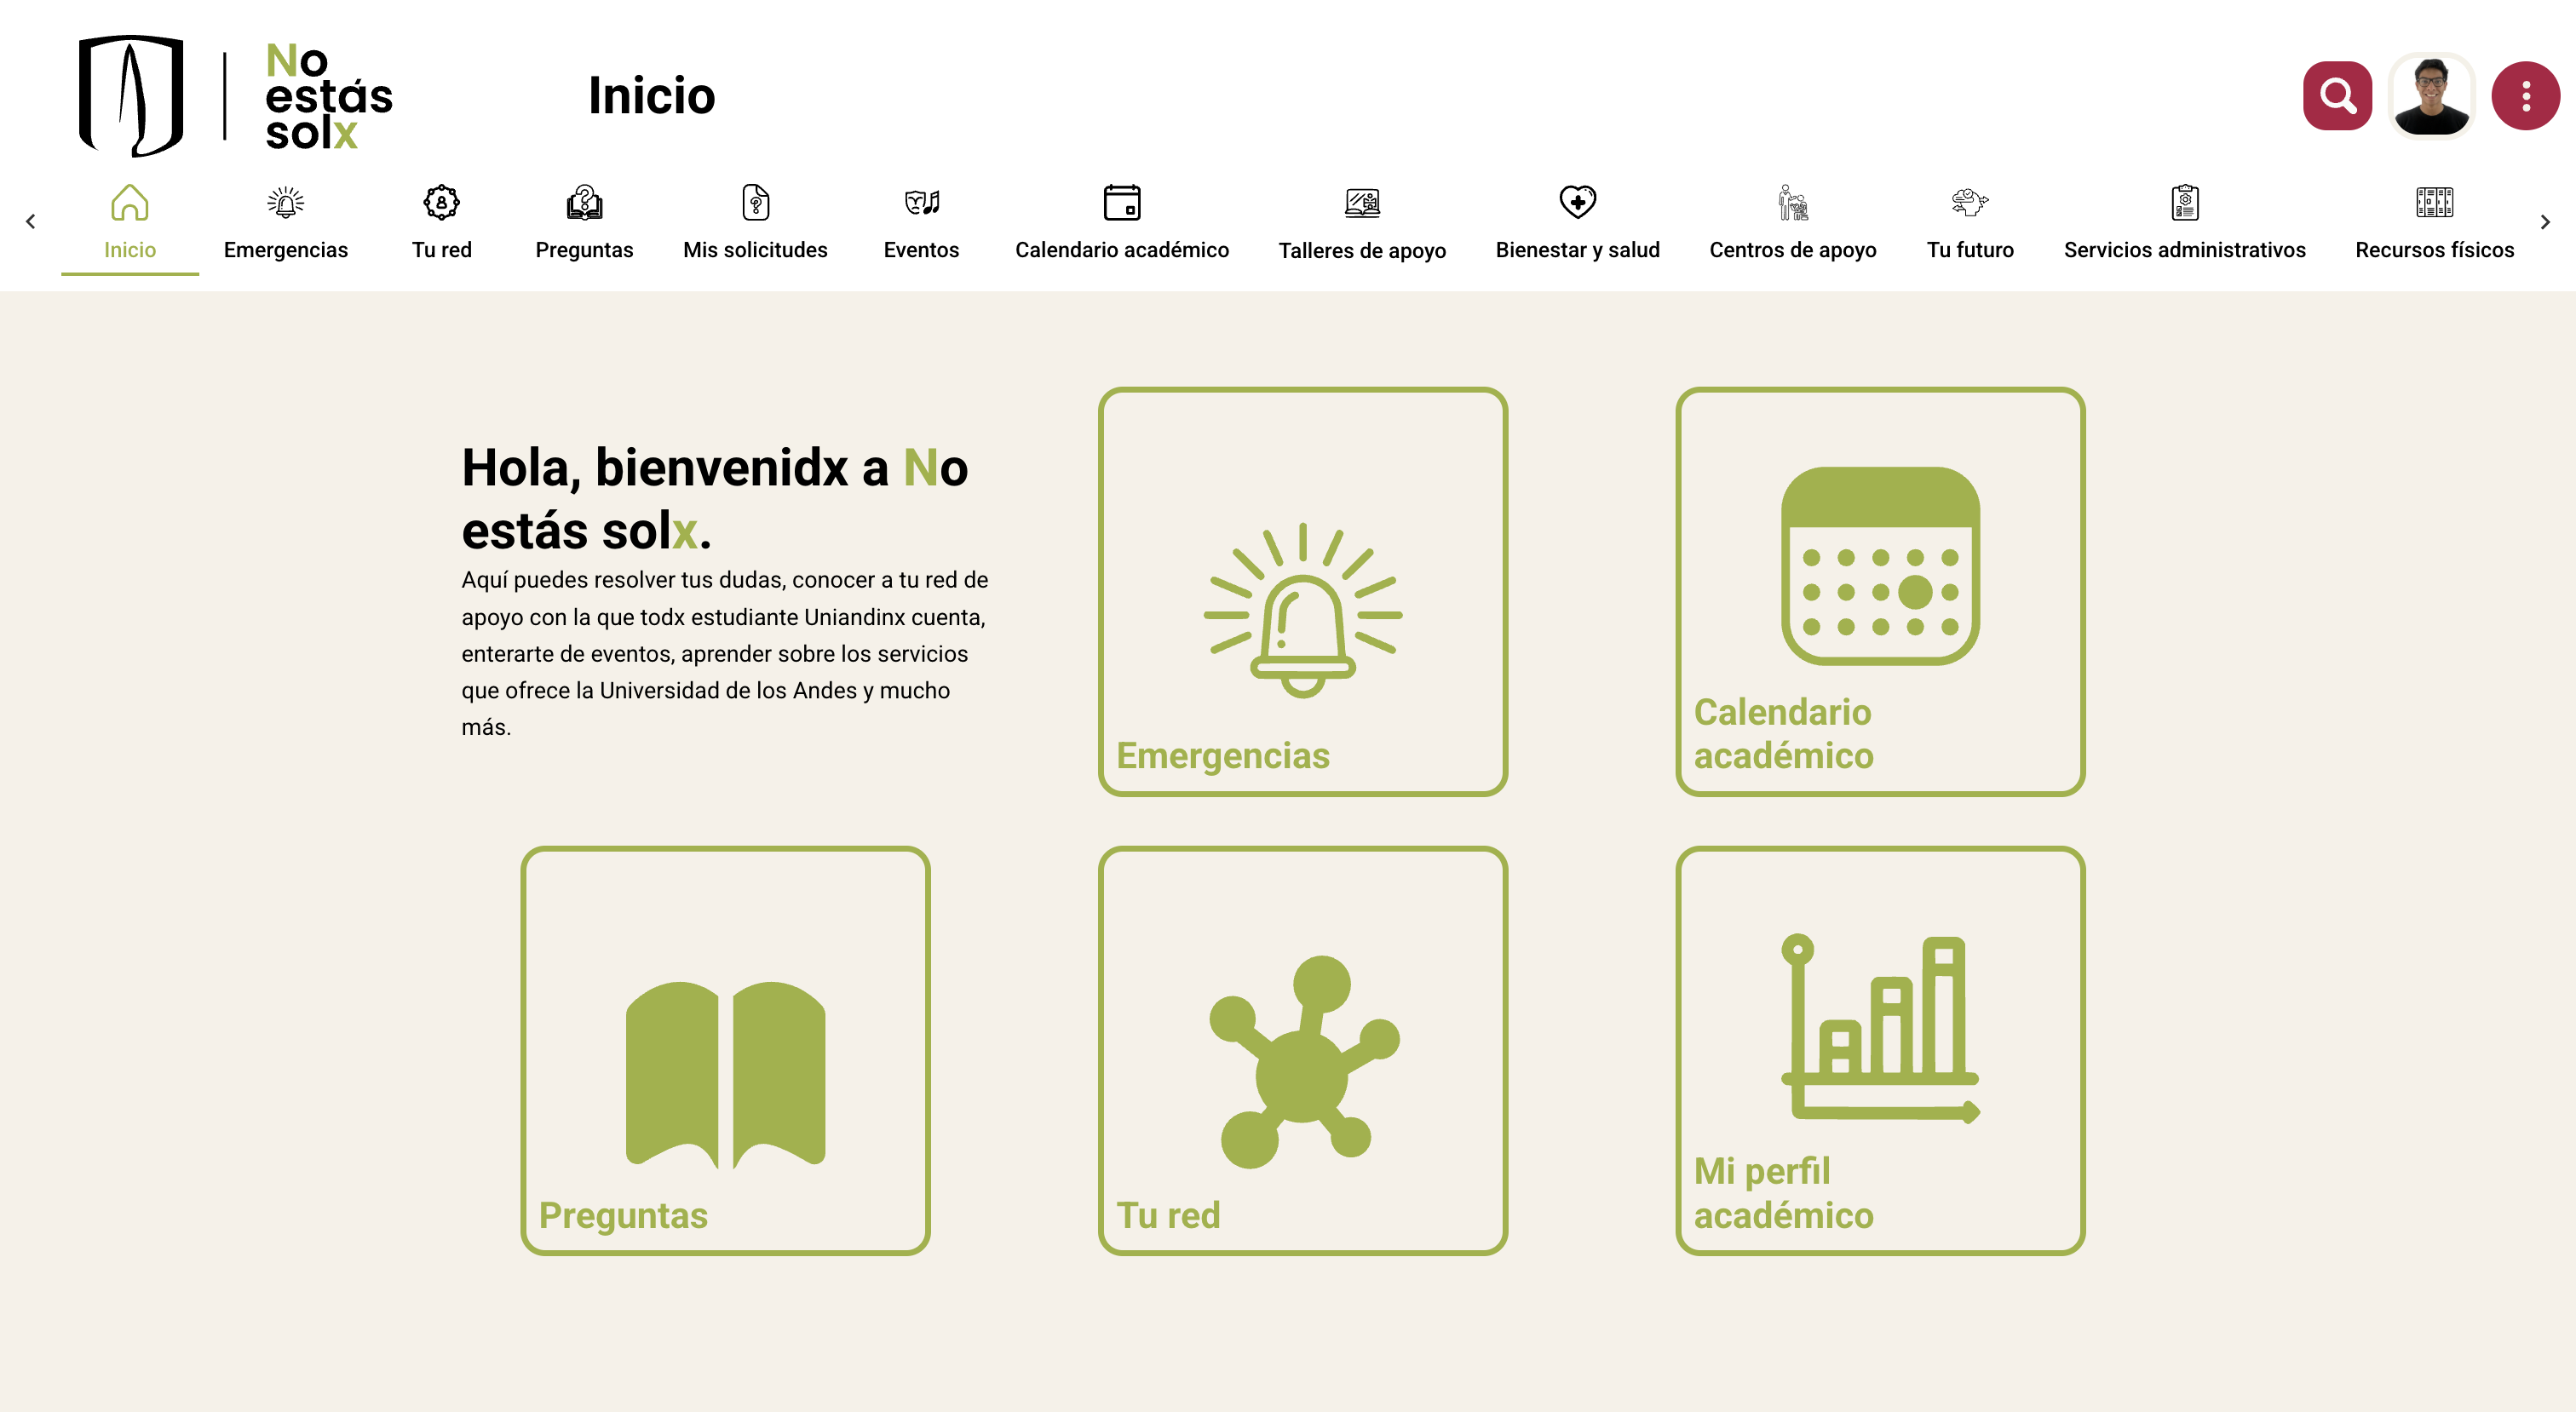
\includegraphics[width=\textwidth]{assets/nes/landing_estudiante.png}
	\caption{Página inicial de NES para un estudiante.}
	\label{fig:landing_estudiante}
\end{figure}

La segunda manera de acceder al Perfil del estudiante como alumno es pulsando en su fotografía, que se ubica en la parte superior derecha de la página inicial de \gls{NES} para estudiantes. Al hacer clic en la fotografía, se despliega la ventana modal que se puede ver en la figura \ref{fig:menu_estudiante}, que incluye la opción \textit{Ver mi perfil académico}. Al pulsar en esta opción, se accede al Perfil del estudiante.

\begin{figure}[H]
	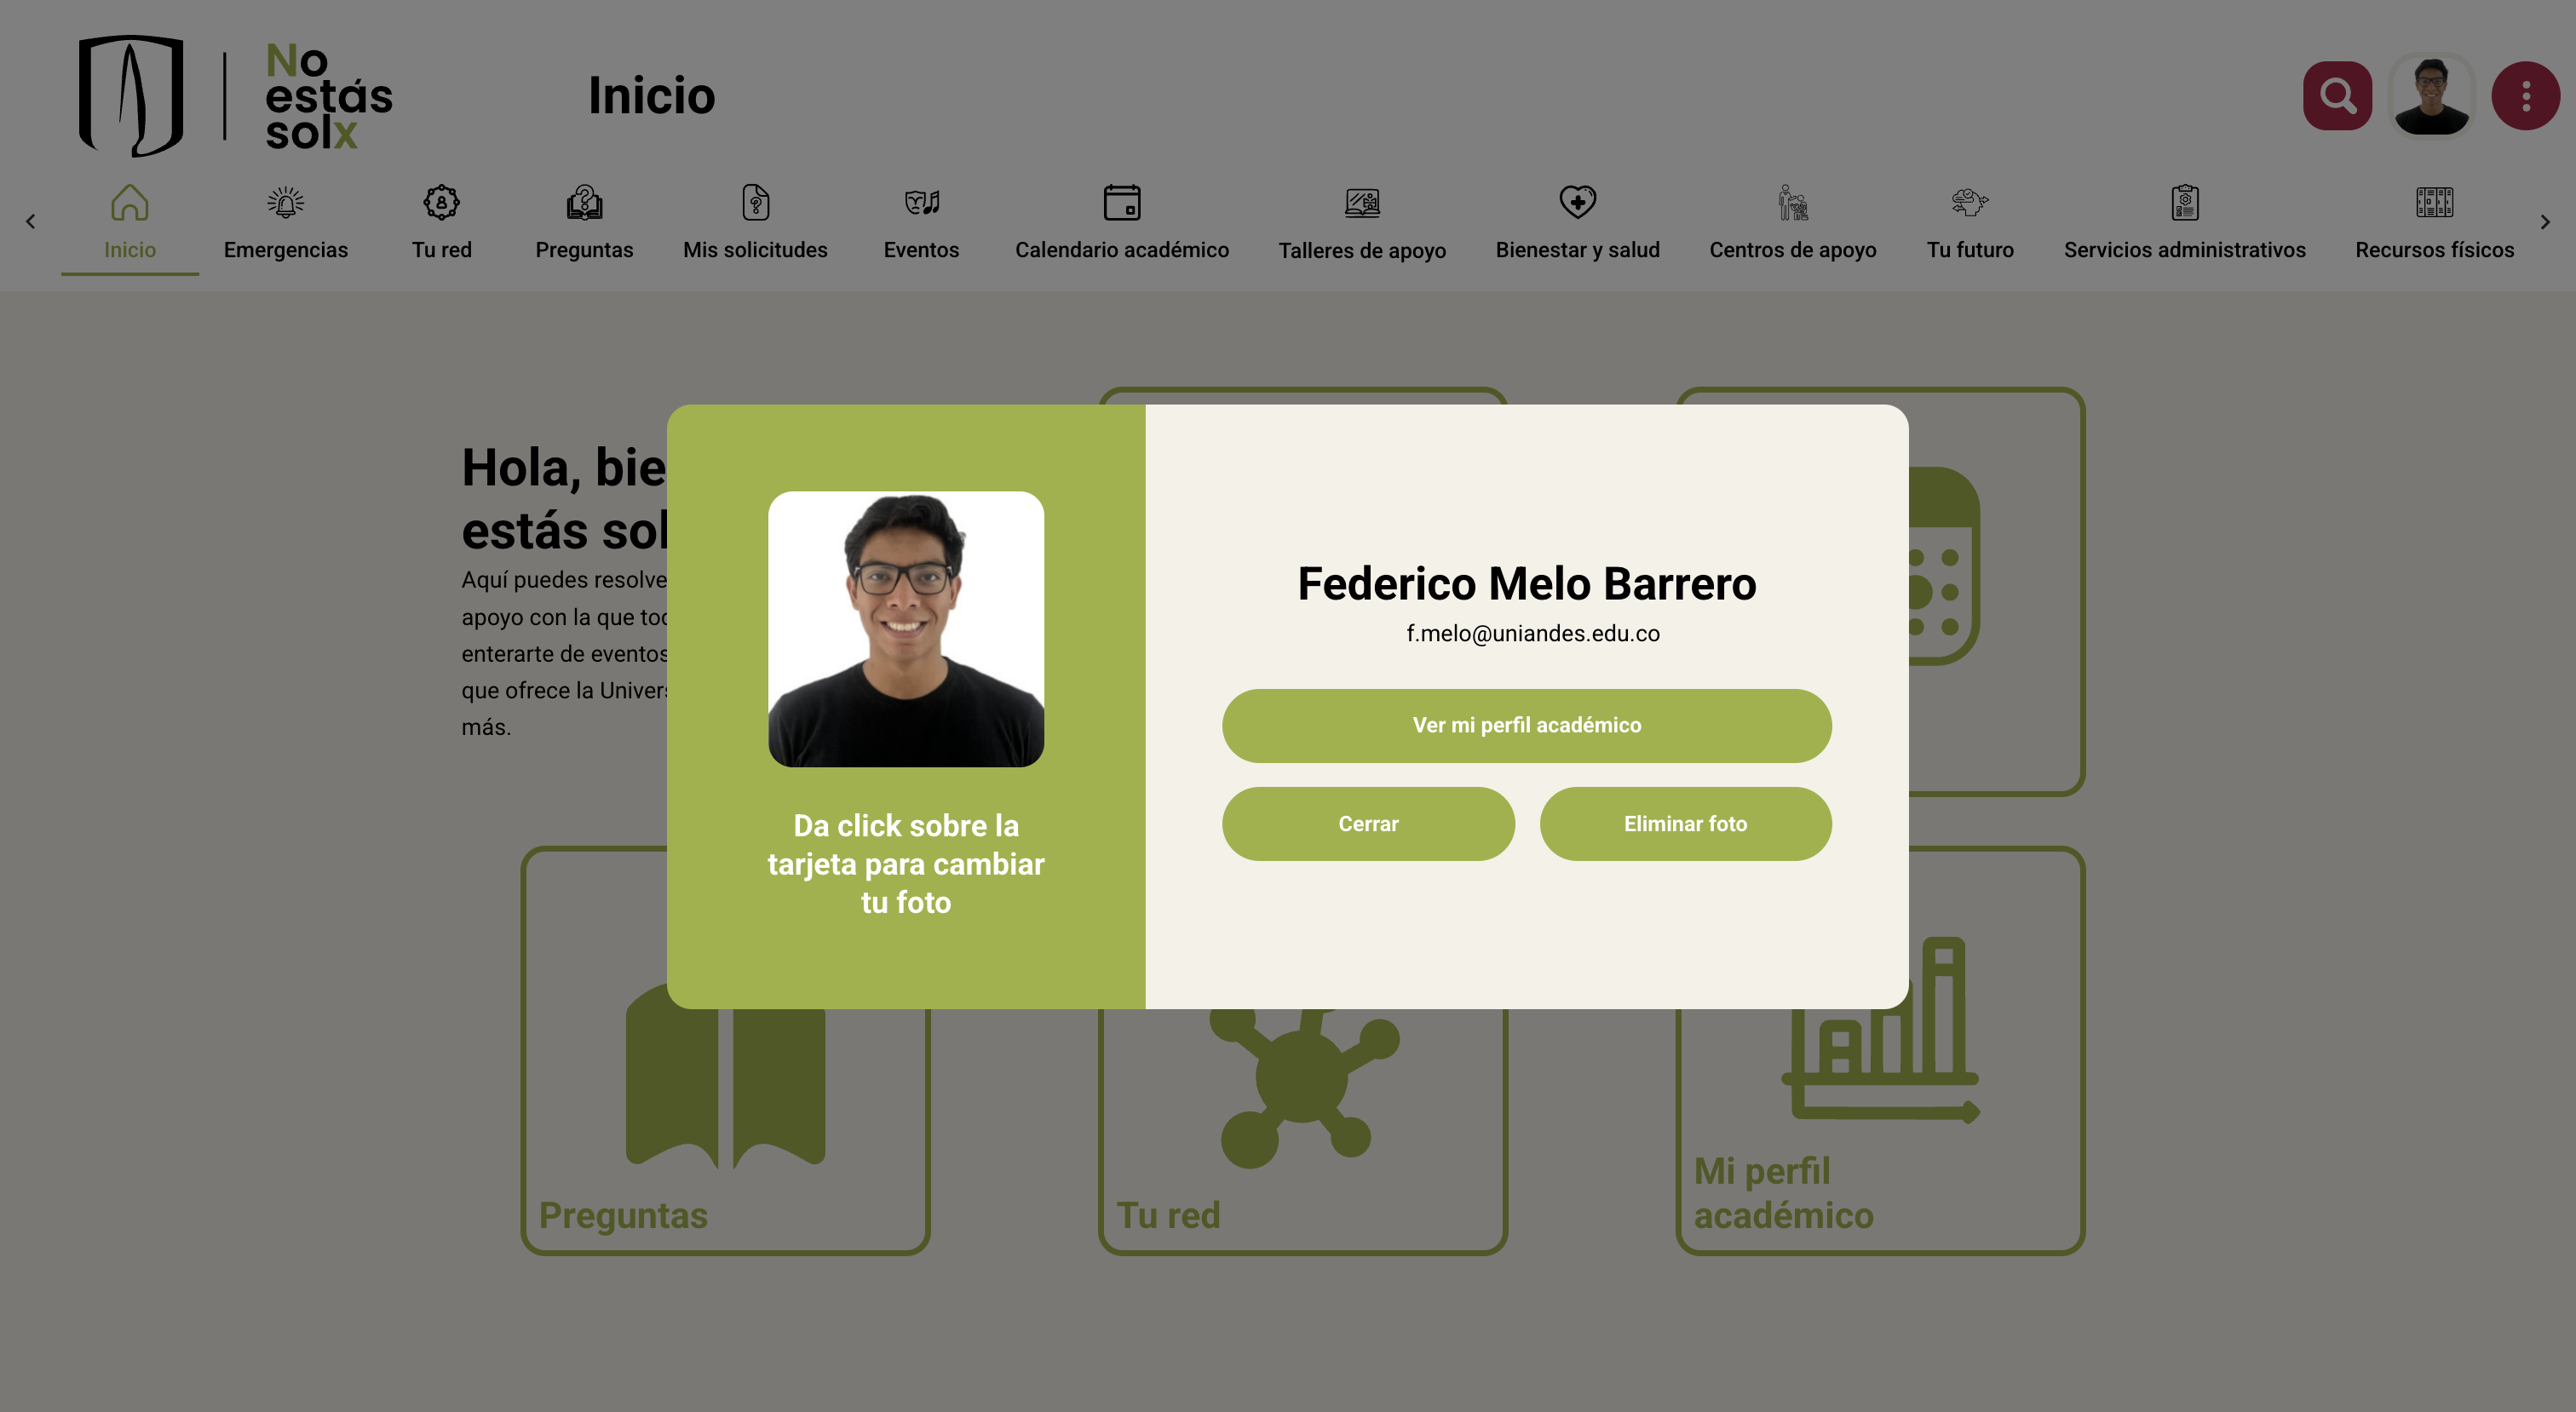
\includegraphics[width=\textwidth]{assets/nes/menu_estudiante.png}
	\caption{Ventana modal de opciones para el estudiante.}
	\label{fig:menu_estudiante}
\end{figure}

\subsubsection{Acceso al Perfil del estudiante como profesor o directivo}

El acceso al perfil del estudiante como profesor o directivo difiere del acceso como alumno principalmente en el hecho de que el profesor o directivo debe seleccionar el estudiante cuyo perfil desea visualizar. Para ello, tras haber iniciado sesión en \gls{NES} con su correo Uniandes y su contraseña, debe dirigirse a la pestaña Tus aconsejados en la barra de navegación superior. Una vez seleccionada esta pestaña, se despliega una lista de estudiantes como la que se muestra en la figura \ref{fig:tus_aconsejados}.

\begin{figure}[H]
	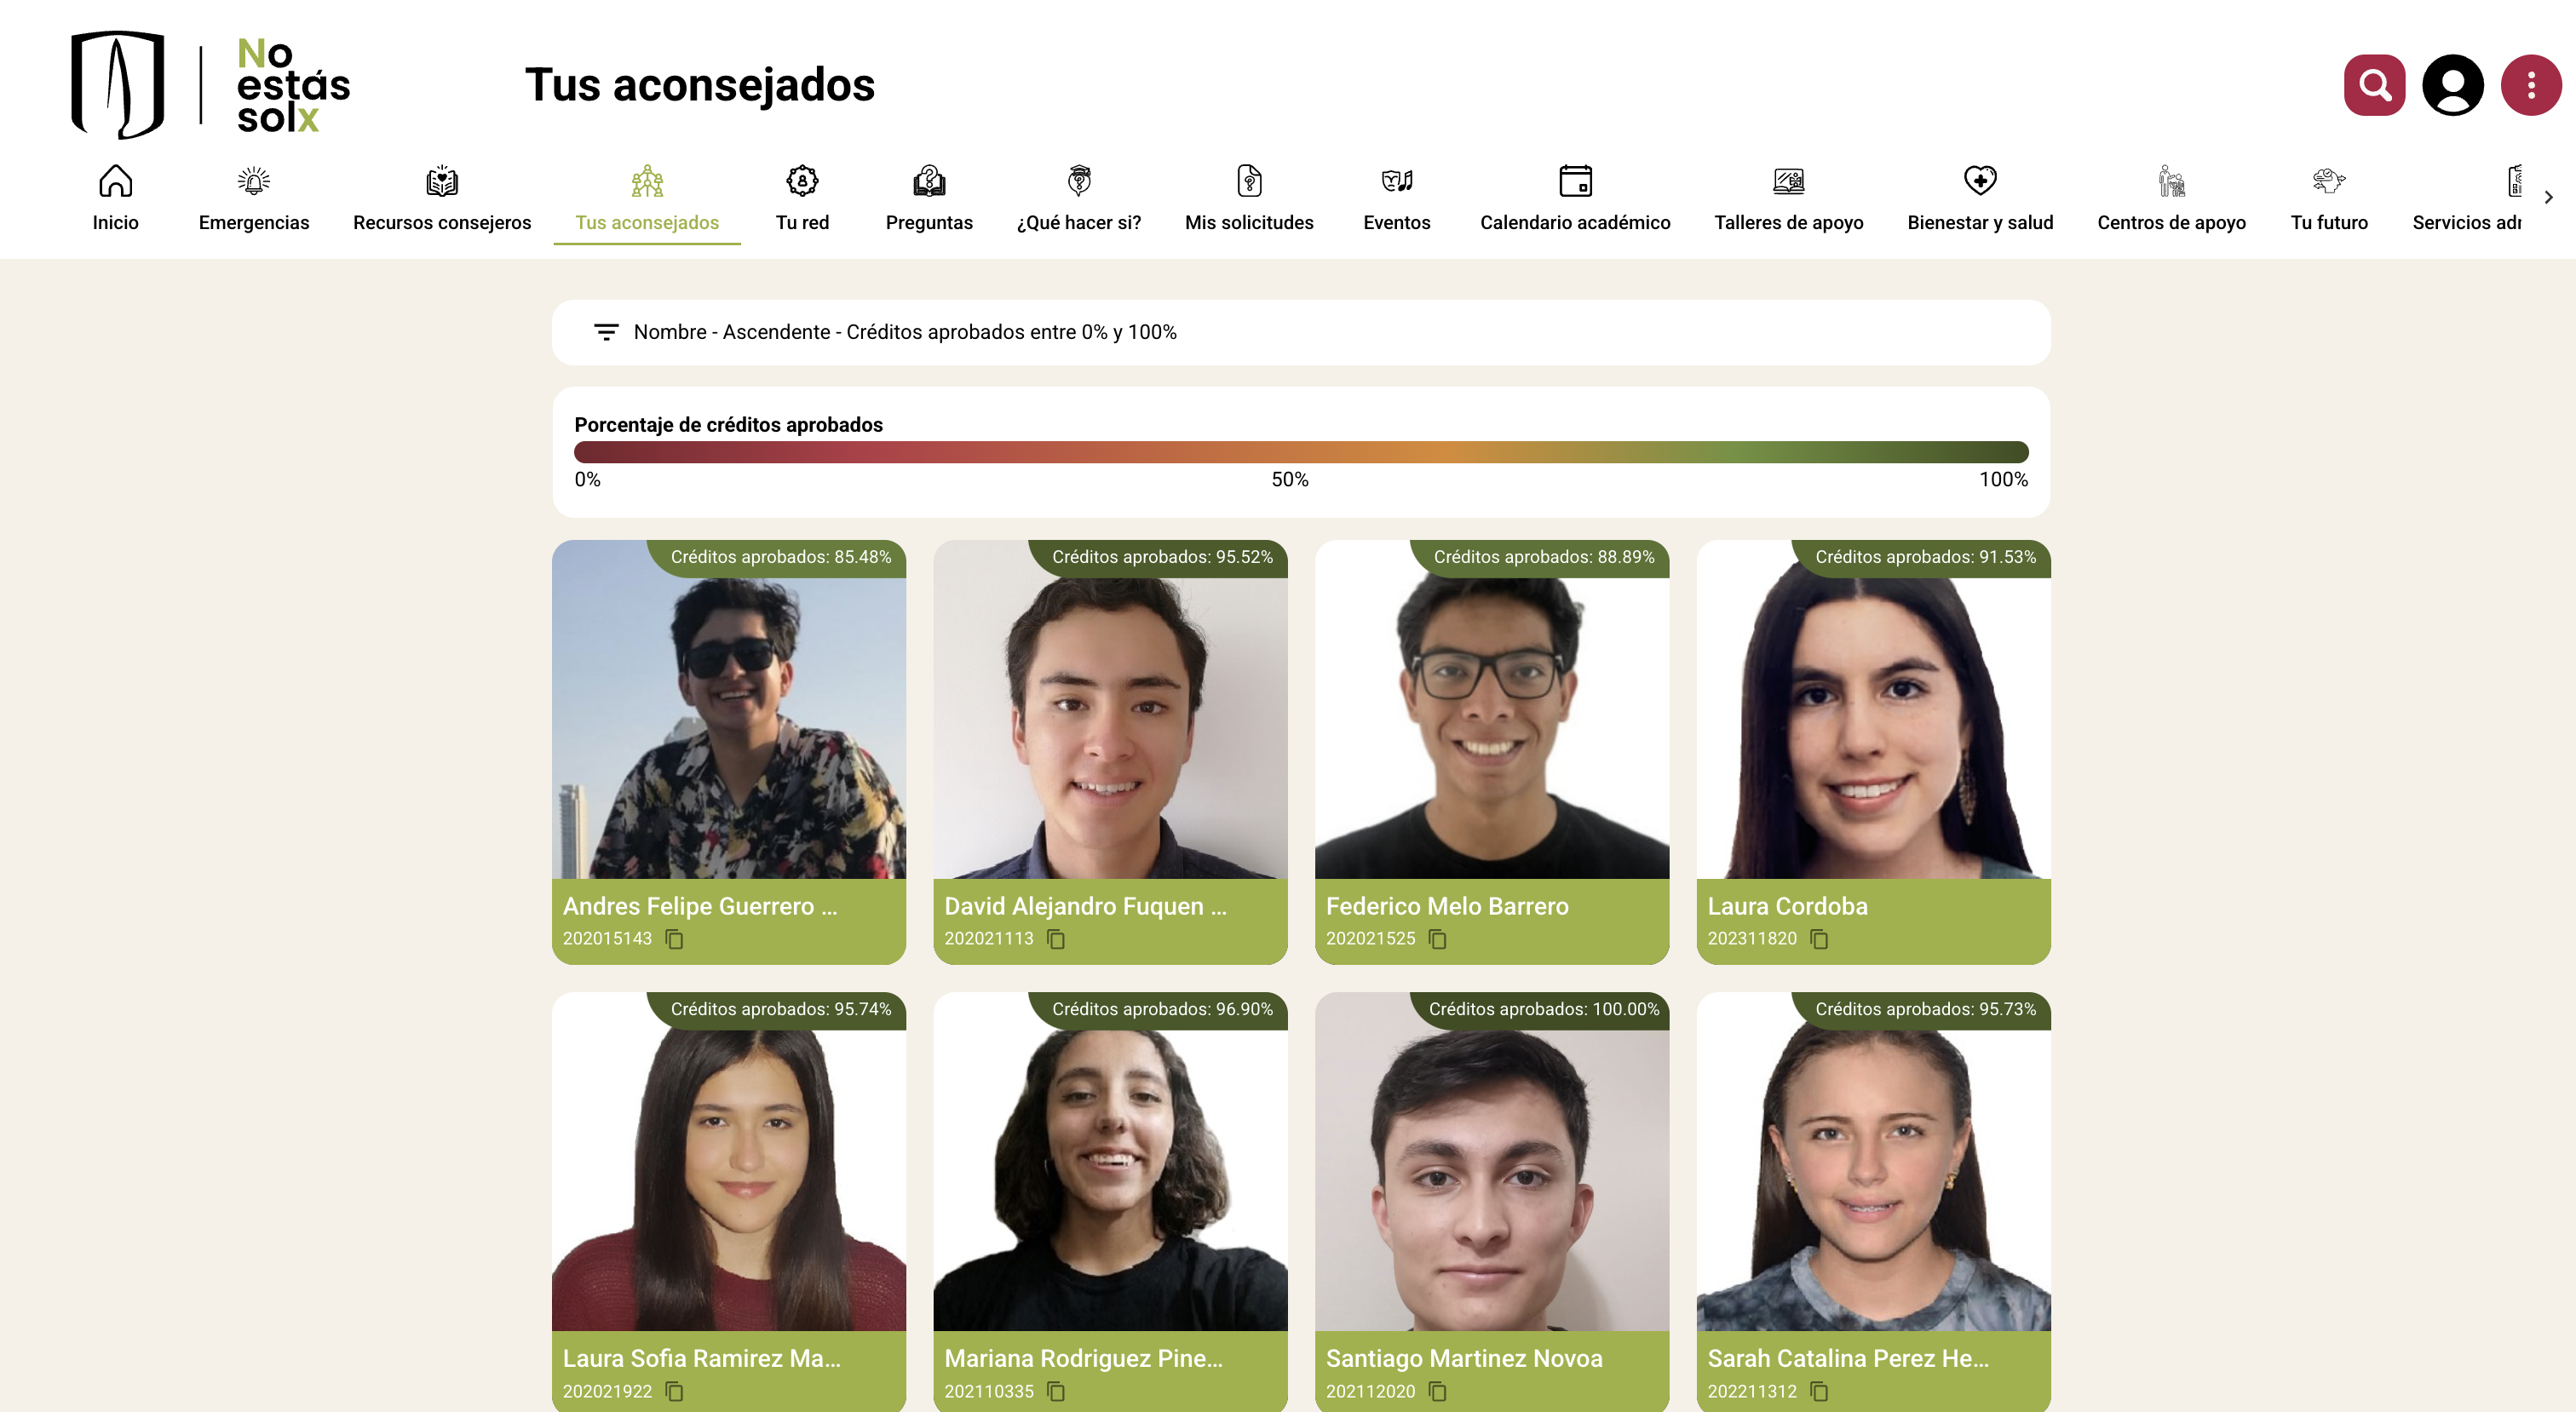
\includegraphics[width=\textwidth]{assets/nes/tus_aconsejados.png}
	\caption{Pestaña Tus aconsejados en NES.}
	\label{fig:tus_aconsejados}
\end{figure}

En esta lista, el profesor o directivo puede seleccionar al alumno cuyo perfil desea visualizar. Al hacer clic sobre la tarjeta que representa a esa persona, se accede al Perfil del estudiante de ese alumno en particular. Los estudiantes que aparecen en ese listado dependen del rol del profesor o directivo en la Universidad, así como de las políticas de gobierno de datos de la Universidad. Para los profesores consejeros, la lista se limita a sus aconsejados. Dependiendo del rol del usuario en cuestión, es posible que pueda hacer uso de la barra de búsqueda en la parte superior derecha de la interfaz para buscar a cualquier estudiante de la Universidad, ya sea por su nombre, por su correo Uniandes o por su código estudiantil.

Más aún, en la pestaña Tus aconsejados, el profesor o directivo puede pulsar en el ícono de tres rayas horizontales, ubicado en la parte superior izquierda, para desplegar un menú lateral con opciones de filtrado, como se muestra en la figura \ref{fig:filtros}. Allí, es posible ordenar los alumnos mostrados por nombre o porcentaje de créditos aprobados, así como utilizar la barra deslizante para fijar un rango de porcentaje de créditos aprobados. Para algunos roles, es posible marcar la opción que permite visualizar a todos los estudiantes de la Universidad, en lugar de solo los aconsejados, con base en las políticas de gobierno de datos de la Universidad.

\begin{figure}[H]
	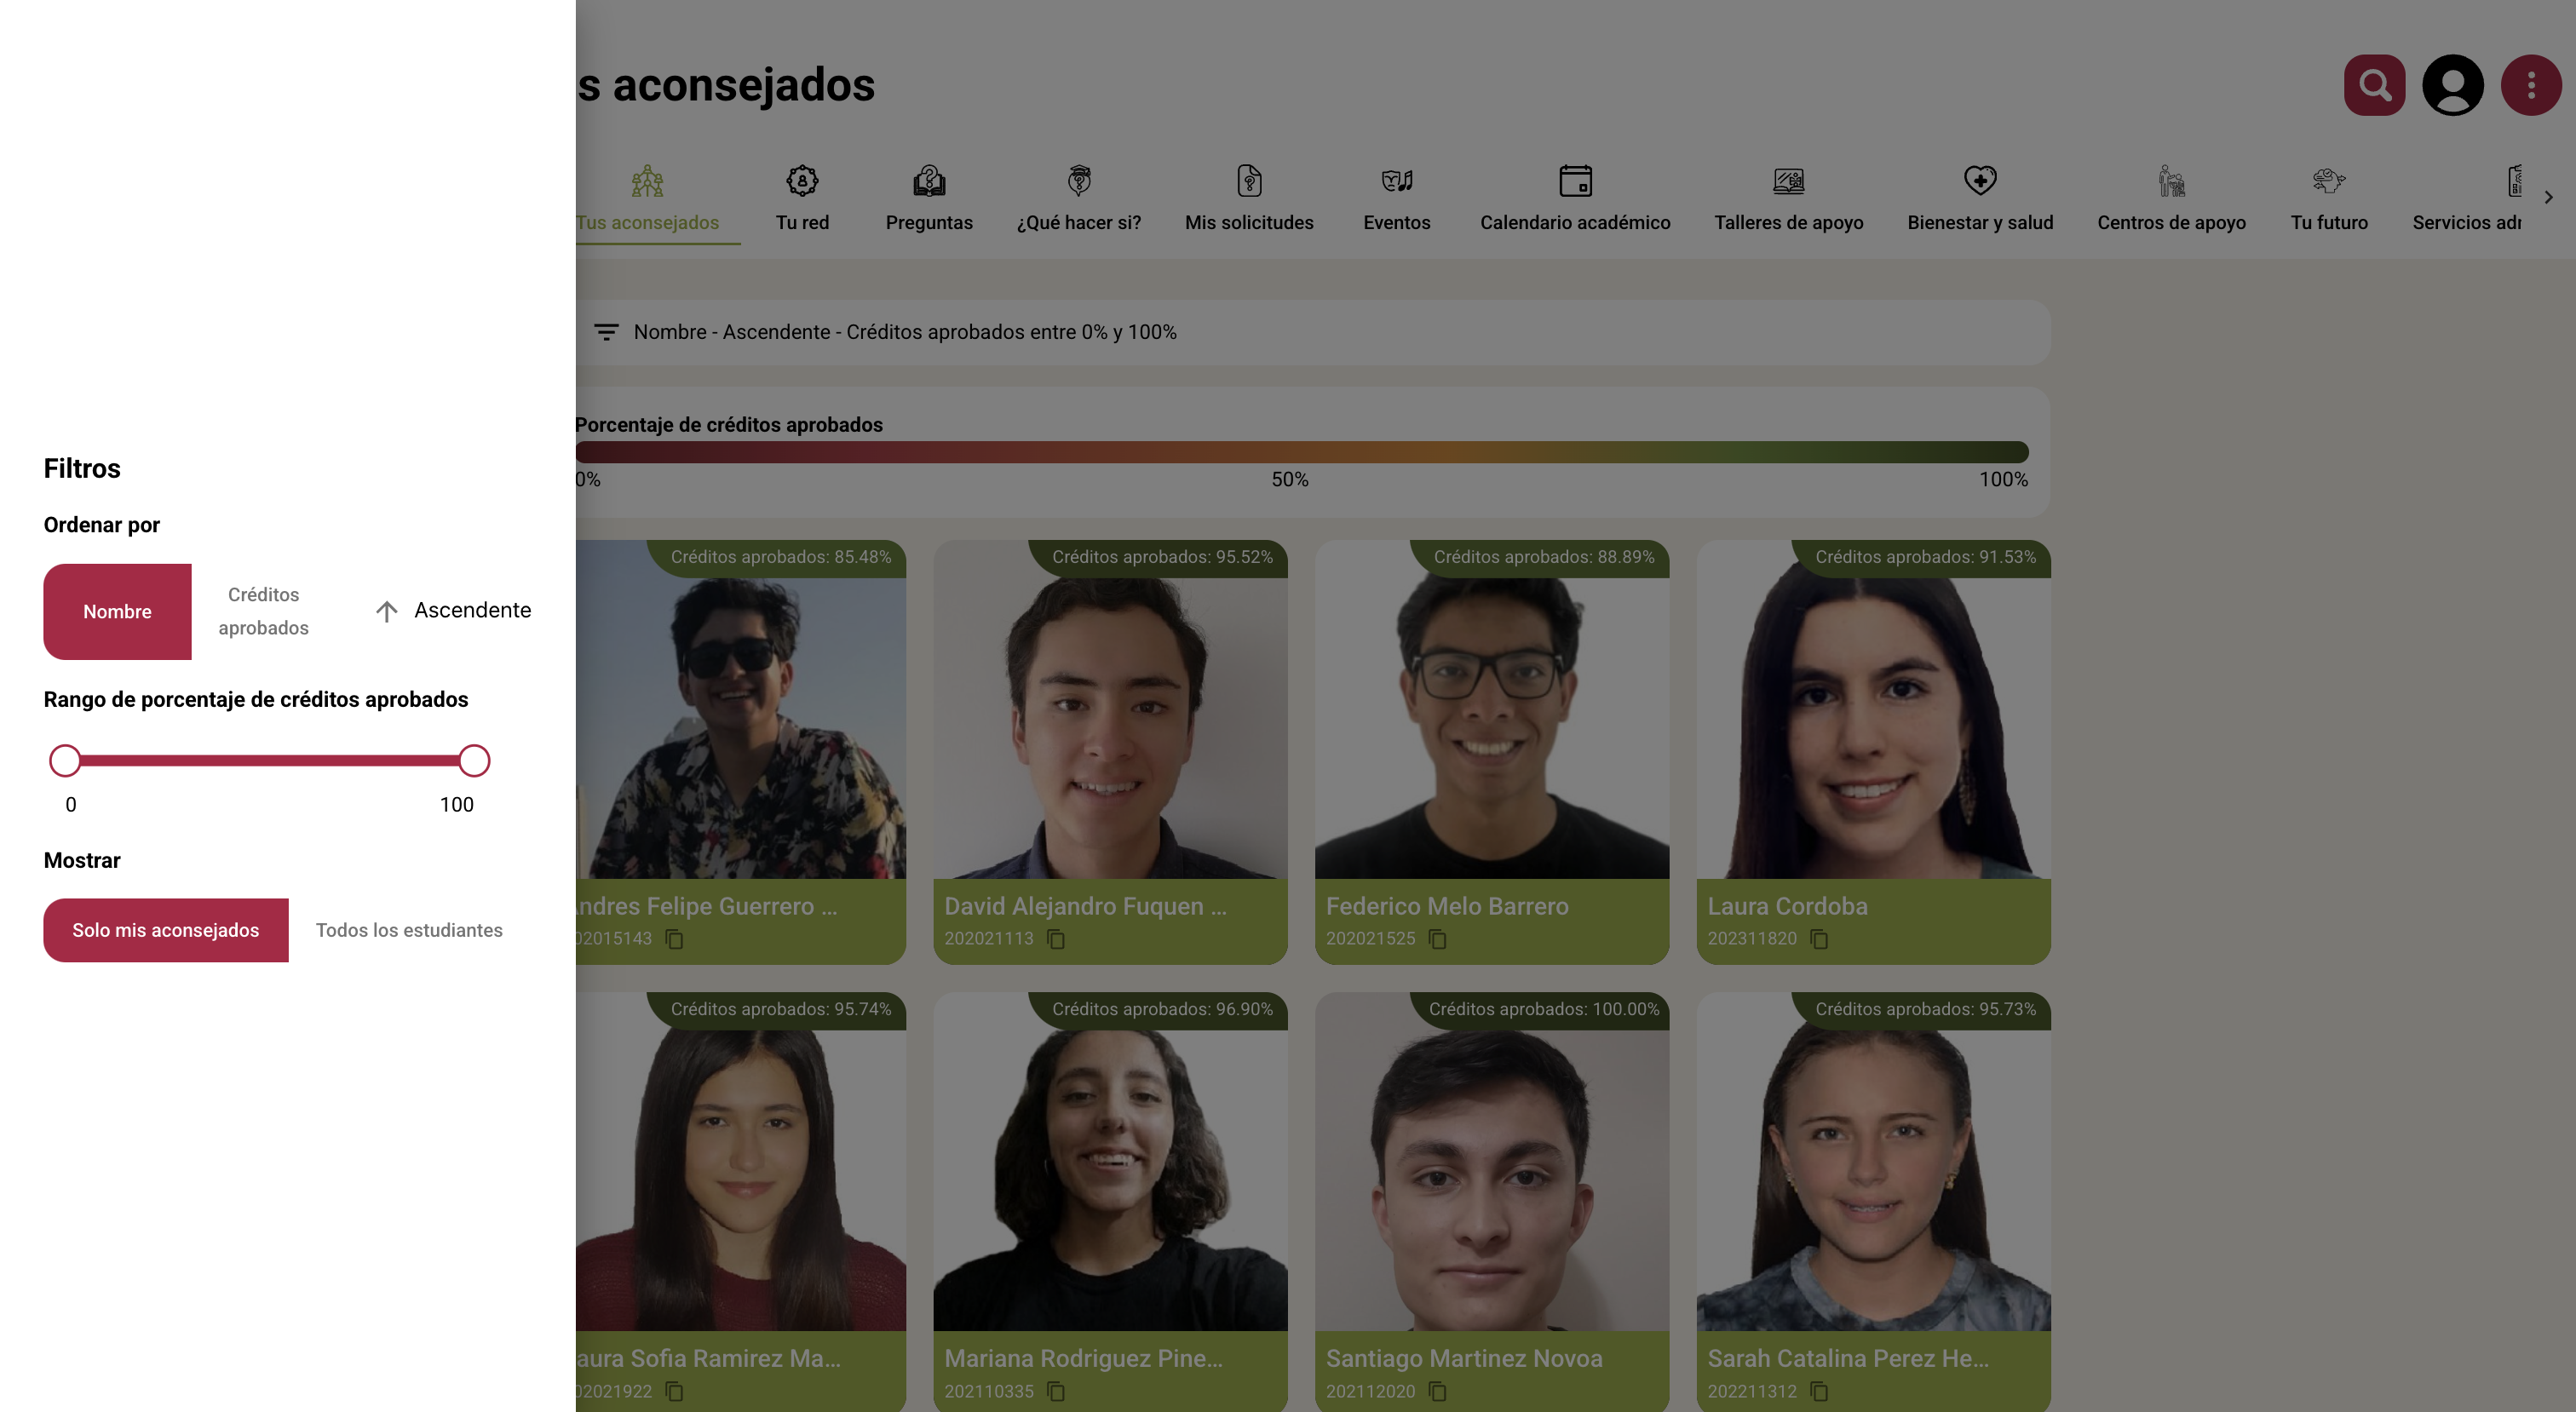
\includegraphics[width=\textwidth]{assets/nes/filtros.png}
	\caption{Menú de filtros en la pestaña Tus aconsejados.}
	\label{fig:filtros}
\end{figure}

\subsection{Disposición general}

El Perfil del estudiante tiene la misma disposición general en cualquiera de sus presentaciones, independiente de si el usuario es un estudiante, un profesor o un directivo. La interfaz se divide en dos secciones principales: a la izquierda, se ubica una tarjeta con información personal del estudiante; a la derecha, se encuentra la pestaña que esté activa. La figura \ref{fig:perfil} muestra la disposición general del Perfil del estudiante con la pestaña Desempeño activa, que es la pestaña por defecto.

\begin{figure}[H]
	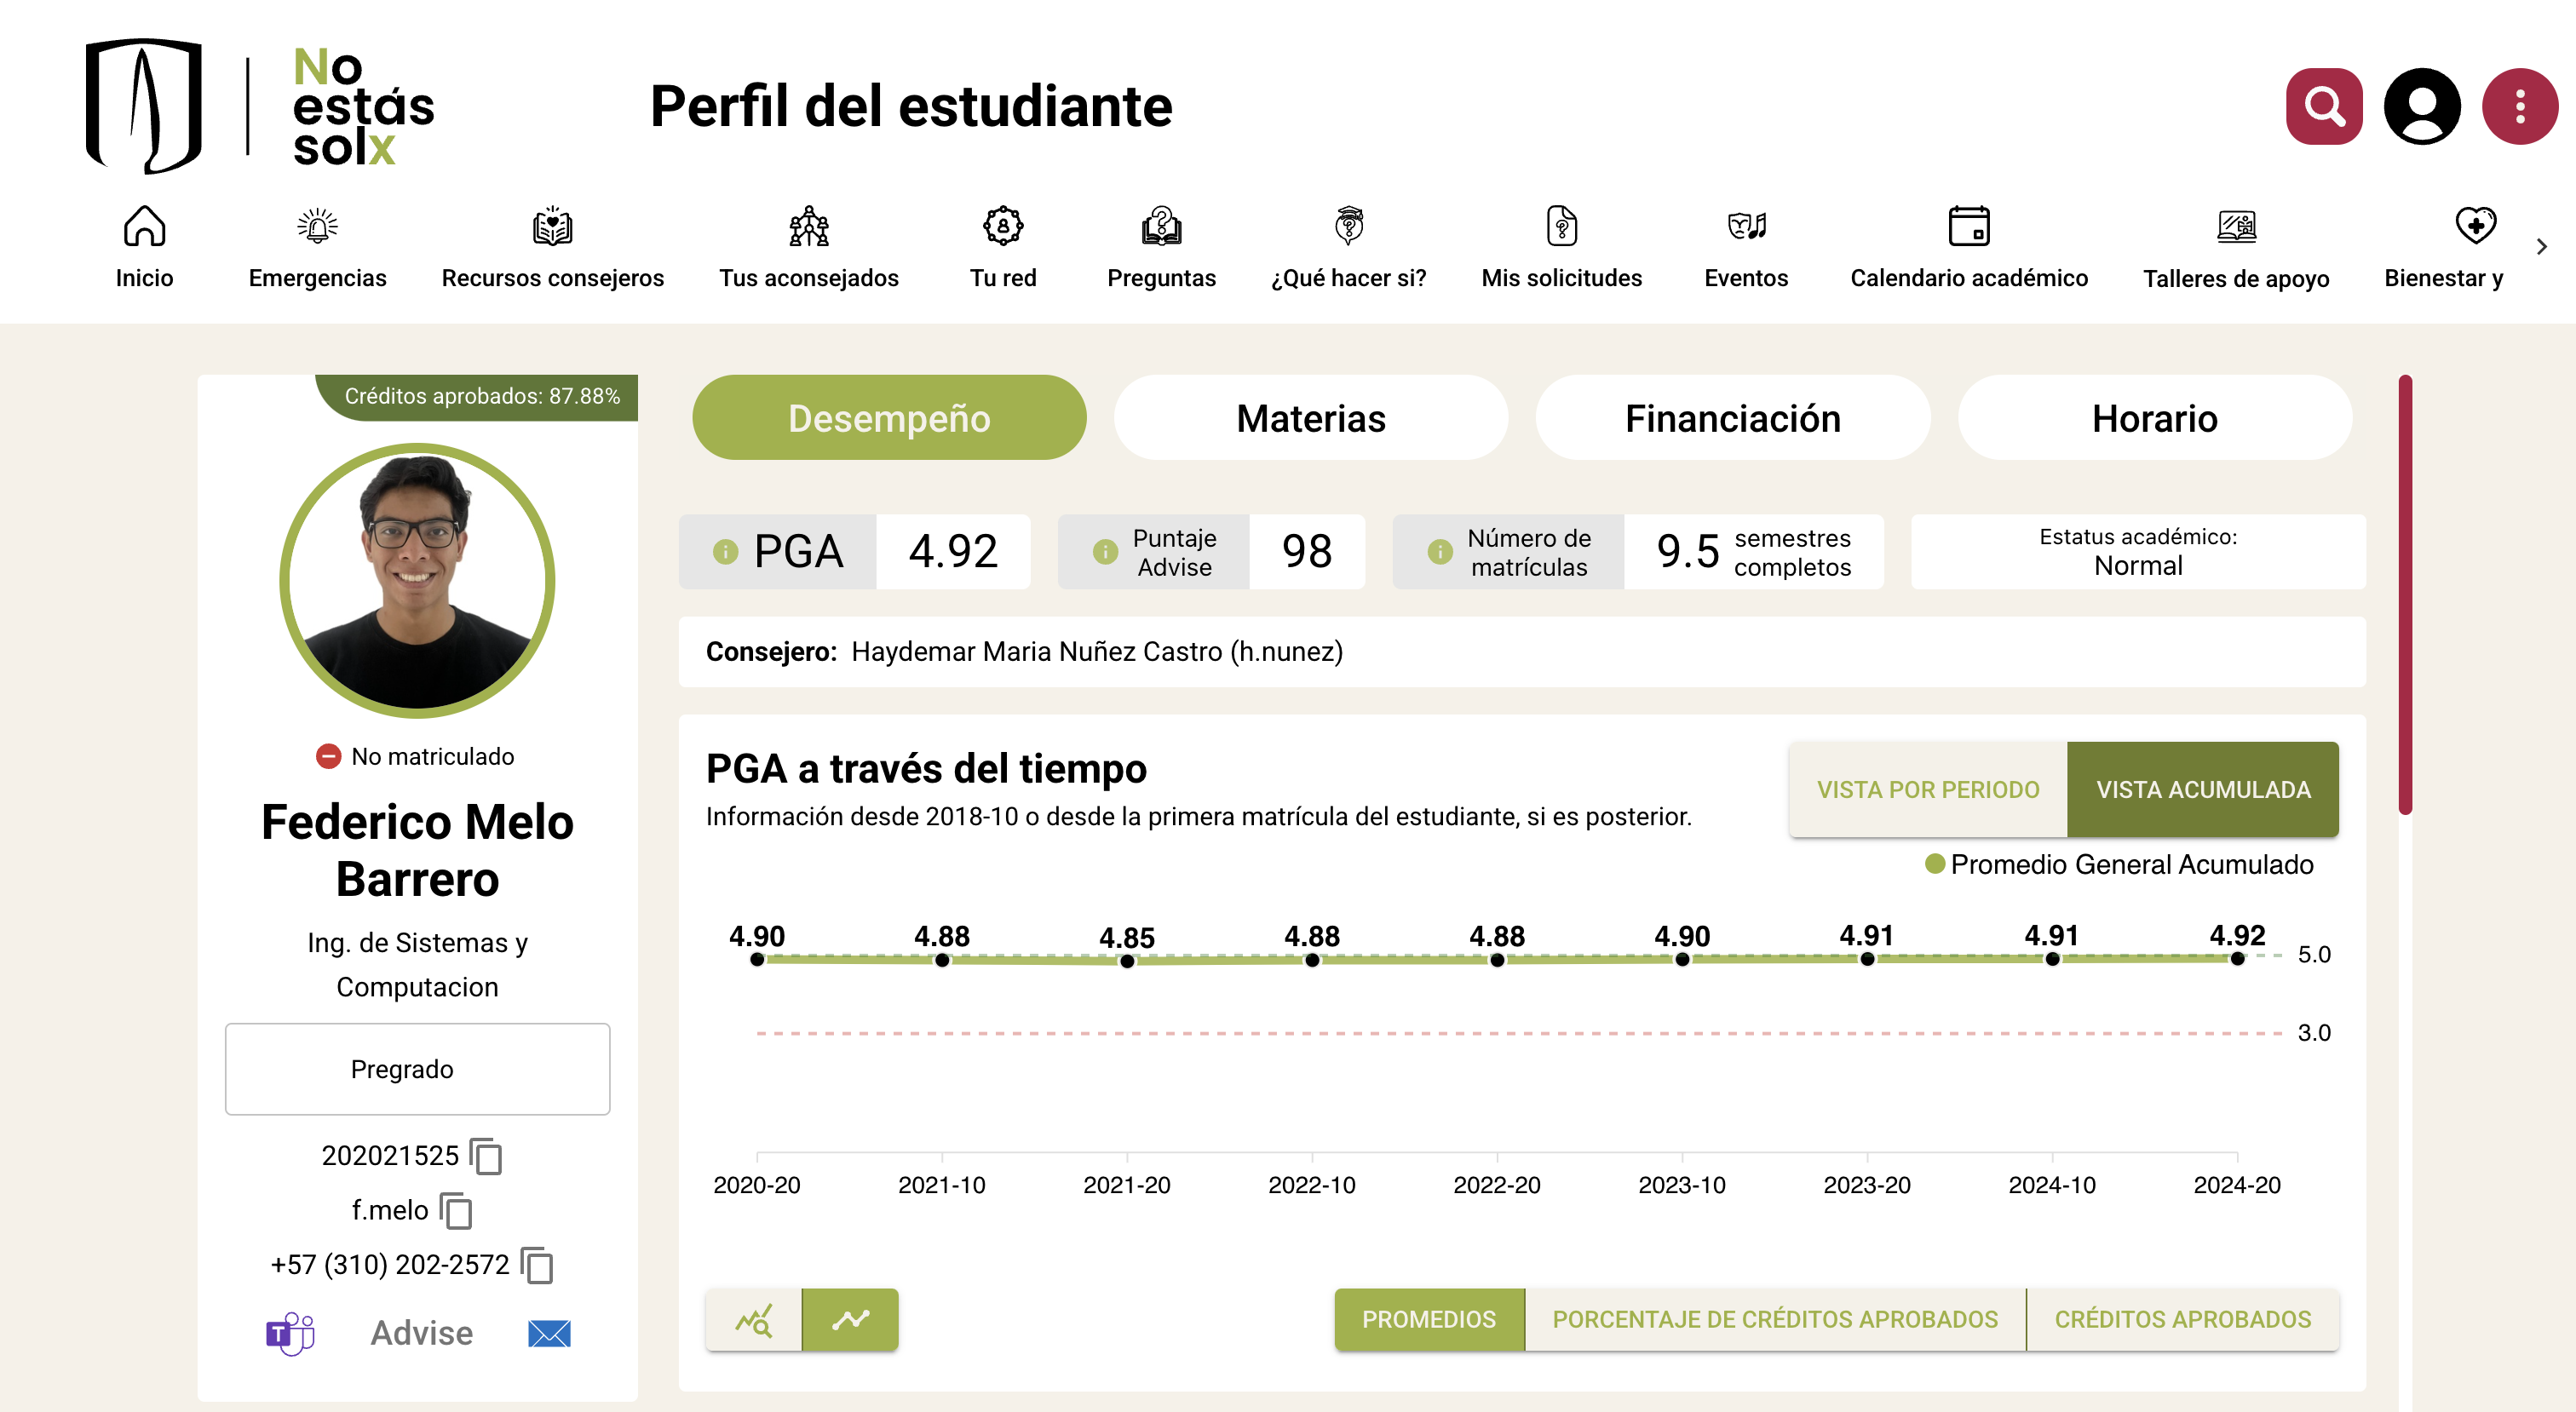
\includegraphics[width=\textwidth]{assets/nes/perfil.png}
	\caption{Disposición general del Perfil del estudiante.}
	\label{fig:perfil}
\end{figure}

La sección de información personal del estudiante contiene toda la información relevante para identificarlo. En la parte superior, se presenta prominentemente la fotografía del alumno, seguida de su nombre completo y el programa académico al que pertenece.

Tras eso, se plasma su nivel académico. En caso de que el estudiante haya estado afiliado a la Universidad en distintos niveles académicos, ese componente se convierte en un selector que permite seleccionar el nivel académico que se desea visualizar, como se muestra en la figura \ref{fix:selector}. Al cambiar el nivel académico, cambia por completo el Perfil del estudiante, pues toda la información presentada en las pestañas se ajusta al nivel académico seleccionado.

\begin{figure}[H]
	\centering
	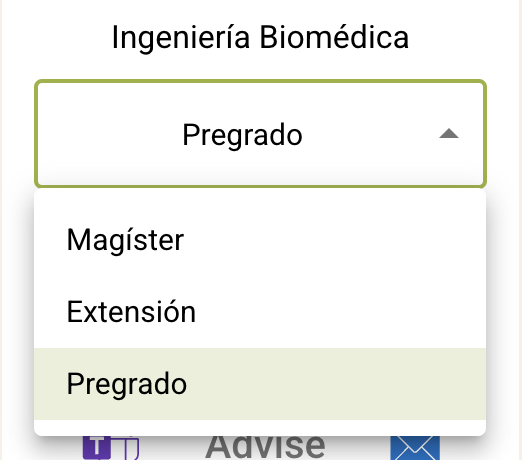
\includegraphics[width=0.4\textwidth]{assets/nes/selector.png}
	\caption{Selector de nivel académico en el perfil de un estudiante anónimo.}
	\label{fix:selector}
\end{figure}

Más abajo, se detallan datos como el código Uniandes del estudiante, su usuario de correo institucional y su número de contacto, este último solo disponible para directivos. Cada uno de esos tres datos tienen a su derecha un botón que facilita copiarlo al portapapeles. Finalmente, se ofrecen botones de interacción directa, como un enlace para asesoramiento mediante Microsoft Teams y otro para enviar correos electrónicos, lo que facilita la comunicación inmediata con el alumno.

La sección de información personal del estudiante está diseñada para que el Perfil gire en torno a la persona. Independientemente de la pestaña activa en la interfaz, los datos personales del alumno permanecen siempre visibles en la parte izquierda de la pantalla. La interfaz dispone de un sistema de scroll independiente para las dos secciones, permitiendo navegar en la pestaña seleccionada sin que se pierda de vista la información principal del estudiante. La fotografía, ubicada de forma prominente, permanece siempre visible y refuerza la conexión humana, recordando en todo momento que detrás de los datos hay una persona con identidad y contexto.

\subsection{Pestañas del Perfil del estudiante}

El Perfil del estudiante se compone de cuatro pestañas principales: Desempeño, Materias, Financiación y Horario. Los nombres de las pestañas son cortos y dicientes: la primera, Desempeño, contiene toda la información asociada al rendimiento académico; la segunda, Materias, consta de un listado exhaustivo de todas las materias inscritas; la tercera, Financiación, presenta información detallada sobre cómo el estudiante ha financiado sus estudios; y la cuarta, Horario, muestra el horario de clases del alumno al momento de la consulta.

Cada una de estas pestañas presenta información relevante para el estudiante, el profesor o el directivo, dependiendo del rol del usuario que accede al Perfil. A continuación, se dedica una sección a cada una de las pestañas, describiendo la información presentada y las funcionalidades disponibles.

\subsubsection{Pestaña de Desempeño}

La pestaña de Desempeño es la pestaña por defecto que se muestra al acceder al Perfil del estudiante. Esta pestaña ofrece un análisis detallado del rendimiento académico a través del tiempo. A continuación, se detallan uno a uno los elementos que componen la pestaña de Desempeño. Para empezar, la figura \ref{fig:desempeno} presenta un primer pedazo de la pestaña de Desempeño, que contiene los indicadores claves y la gráfica central.

\begin{figure}[H]
	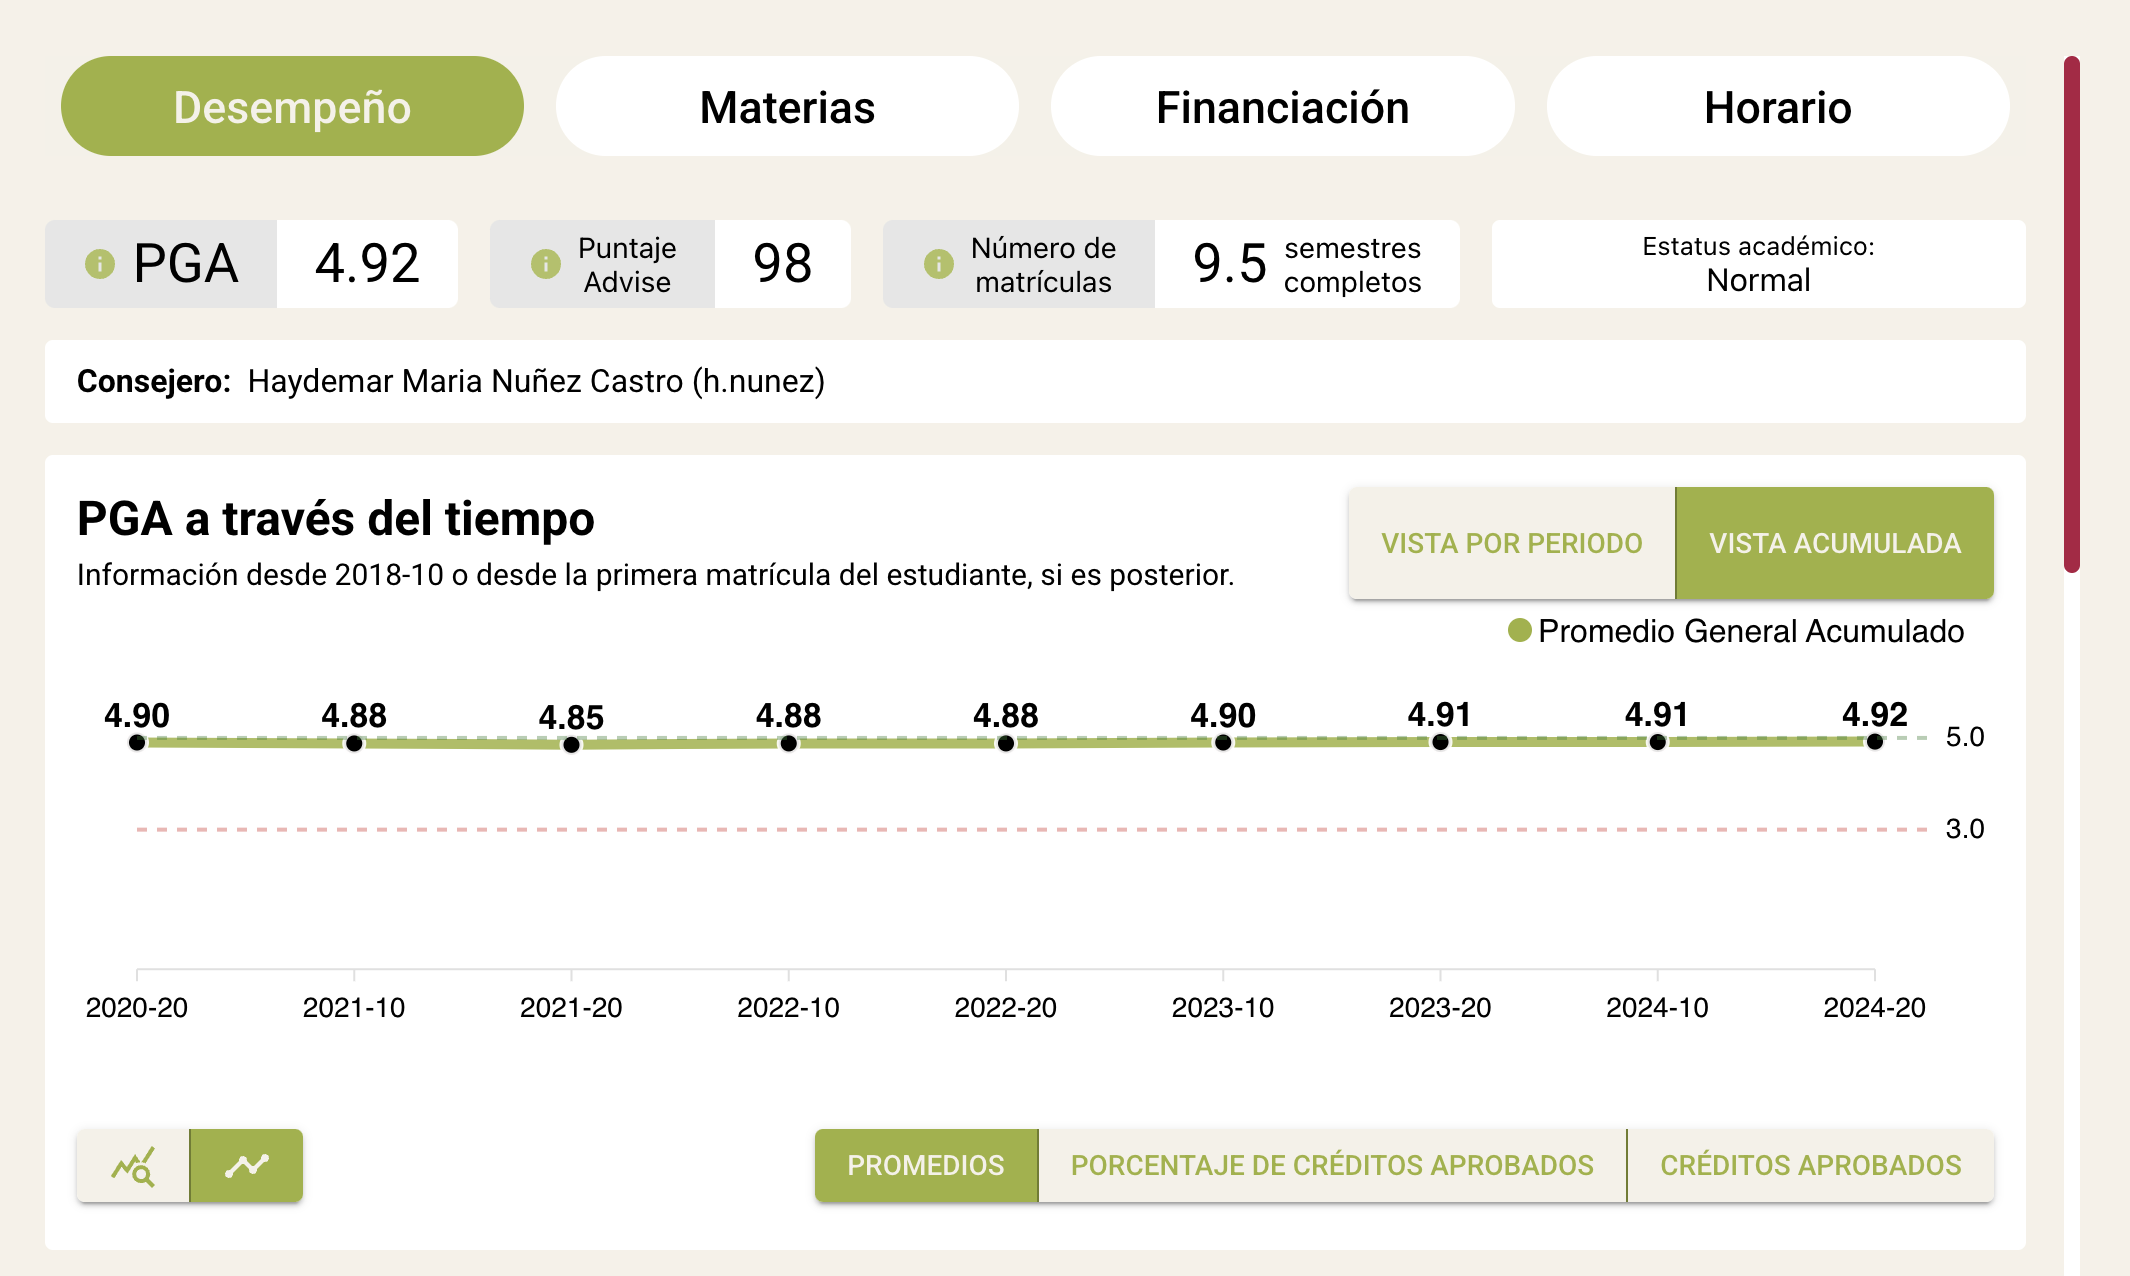
\includegraphics[width=\textwidth]{assets/nes/desempeno_1.png}
	\caption{Parte de arriba de la pestaña de Desempeño.}
	\label{fig:desempeno}
\end{figure}

\paragraph{Indicadores clave} En la parte superior de la pestaña, se encuentran cuatro indicadores clave que resumen el desempeño académico: el Promedio General Acumulado (PGA), el Puntaje Advise, el número de matrículas que ha realizado y el estado académico actual del estudiante.
\begin{itemize}
	\item El PGA es el principal indicador de rendimiento académico en la Universidad. De acuerdo con el Reglamento general de estudiantes de pregrado de la Universidad de los Andes, el PGA resulta de multiplicar el número de créditos de cada materia por la calificación obtenida, sumando estos productos y dividiendo el resultado por el número total de créditos calificados numéricamente.
	      % TODO: Cita
	      Su menor valor es 1.5 y su máximo valor es 5.0. El PGA se presenta con dos decimales.
	\item El Puntaje Advise es un indicador de la probabilidad de éxito académico del estudiante en la Universidad. Es calculado y provisto por la herramienta de análisis predictivo Advise y oscila entre 0 y 100. Se presenta el puntaje Advise tal y como se extrae de la herramienta.
	\item El número de matrículas representa la cantidad de semestres completos que han sido pagados y matriculados. Puede ser un número decimal, en caso de que el alumno haya cursado matrículas parciales. En esta medida, un semestre completo se valora como una matrícula; media matrícula se valora como 0.5 matrículas; y un cuarto de matrícula, un periodo intersemestral o una práctica académica se valora como 0.25 matrículas. Esta medida es un buen reflejo de la inversión realizada en la educación del estudiante.
	\item El estado académico actual del alumno es un término que resume su situación académica, sobretodo para alertar sobre posibles problemas. El valor por defecto es Normal, pero algunos de los posibles valores son: Suspensión académica, Supensión disciplinaria, Prueba académica, Prueba disciplinaria, entre otros.
\end{itemize}

Estos indicadores son la primera pieza de información que el usuario ve al acceder al Perfil del estudiante y le permiten tener una visión general de su rendimiento de un vistazo. Al pasar el cursor sobre cada uno de los indicadores, se despliega una descripción detallada del indicador, que facilita su interpretación. Un ejemplo de esto se presenta en la figura \ref{fig:indicadores}, en la que se pasa el cursor por encima del indicador de Puntaje Advise.

\begin{figure}[H]
	
\includegraphics[width=\textwidth]{assets/nes/indicadores.png}
	\caption{Descripción del indicador de Puntaje Advise al pasar el cursor sobre él.}
	\label{fig:indicadores}
\end{figure}

\paragraph{Profesor consejero} Inmediatamente debajo de los indicadores clave, se muestra el nombre del consejero académico asignado al alumno. El consejero académico es un profesor de la Universidad, comisionado para asesorar a la persona en temas académicos y administrativos, y que puede ser contactado por ella en caso de necesitar orientación. A los estudiantes que cursan múltiples programas académicos se les asigna un consejero académico por cada programa. El raciocinio detrás de mostrar el consejero académico en una posición tan prominente de la pestaña radica en responsabilizar al consejero académico de la orientación del aconsejado y de su rendimiento académico, en particular cuando este ingrese a visualizar el Perfil del estudiante.

\paragraph{Gráfica central} A continuación, se encuentra una gráfica interactiva. Esta gráfica es la pieza central de la pestaña de Desempeño y realmente podría desglosarse en doce gráficas distintas. La interactividad de la gráfica es lo que permite que pueda tener muchas presentaciones distintas sin resultar abrumadora. Para explicar la gráfica, en primer lugar se listan las opciones de interacción que esta ofrece y tras eso se listan las 12 visualizaciones distintas que puede presentar al elegir determinadas opciones de interacción.

Respecto a las opciones de interacción, para variar entre las presentaciones de la gráfica, se presentan tres grupos de botones:
\begin{itemize}
	\item En la parte inferior derecha de la gráfica, se encuentra un botón que permite seleccionar la información que la gráfica despliega. Las posibles opciones son: Promedios, Porcentaje de Créditos Aprobados y Créditos Aprobados.
	\item En la parte superior derecha, se encuentra un botón que permite alternar entre la Vista por periodo y la Vista acumulada.
	\item En la parte inferior izquierda, se encuentra un botón que permite alternar entre dos escalas de la gráfica: la escala estándar, que depende del tipo de información seleccionada, y la escala relativa, que facilita la visualización del comportamiento de la información a través del tiempo.
\end{itemize}

Cada combinación de botones seleccionada resulta en una visualización distinta de la gráfica. A continuación, se listan las 12 visualizaciones distintas que puede presentar la gráfica:
\begin{enumerate}
	\item \textbf{Promedios, Vista acumulada, Escala estándar.} Esta visualización se titula \say{PGA a través del tiempo} y muestra la evolución del Promedio General Acumulado (PGA) del estudiante a lo largo del tiempo, en una escala estándar cuyo valor mínimo es 1.5 y cuyo valor máximo es 5.0. Cada punto de la gráfica representa el PGA del estudiante en un periodo académico específico. En la escala estándar se dibujan dos líneas de referencia: la inferior corresponde al PGA mínimo y se traza en rojo a la altura del 3.0; la superior corresponde al PGA máximo y se traza en verde a la altura del 5.0. Se presenta en la figura \ref{fig:pga_estandar}.

	      \begin{figure}[H]
		      \centering
		      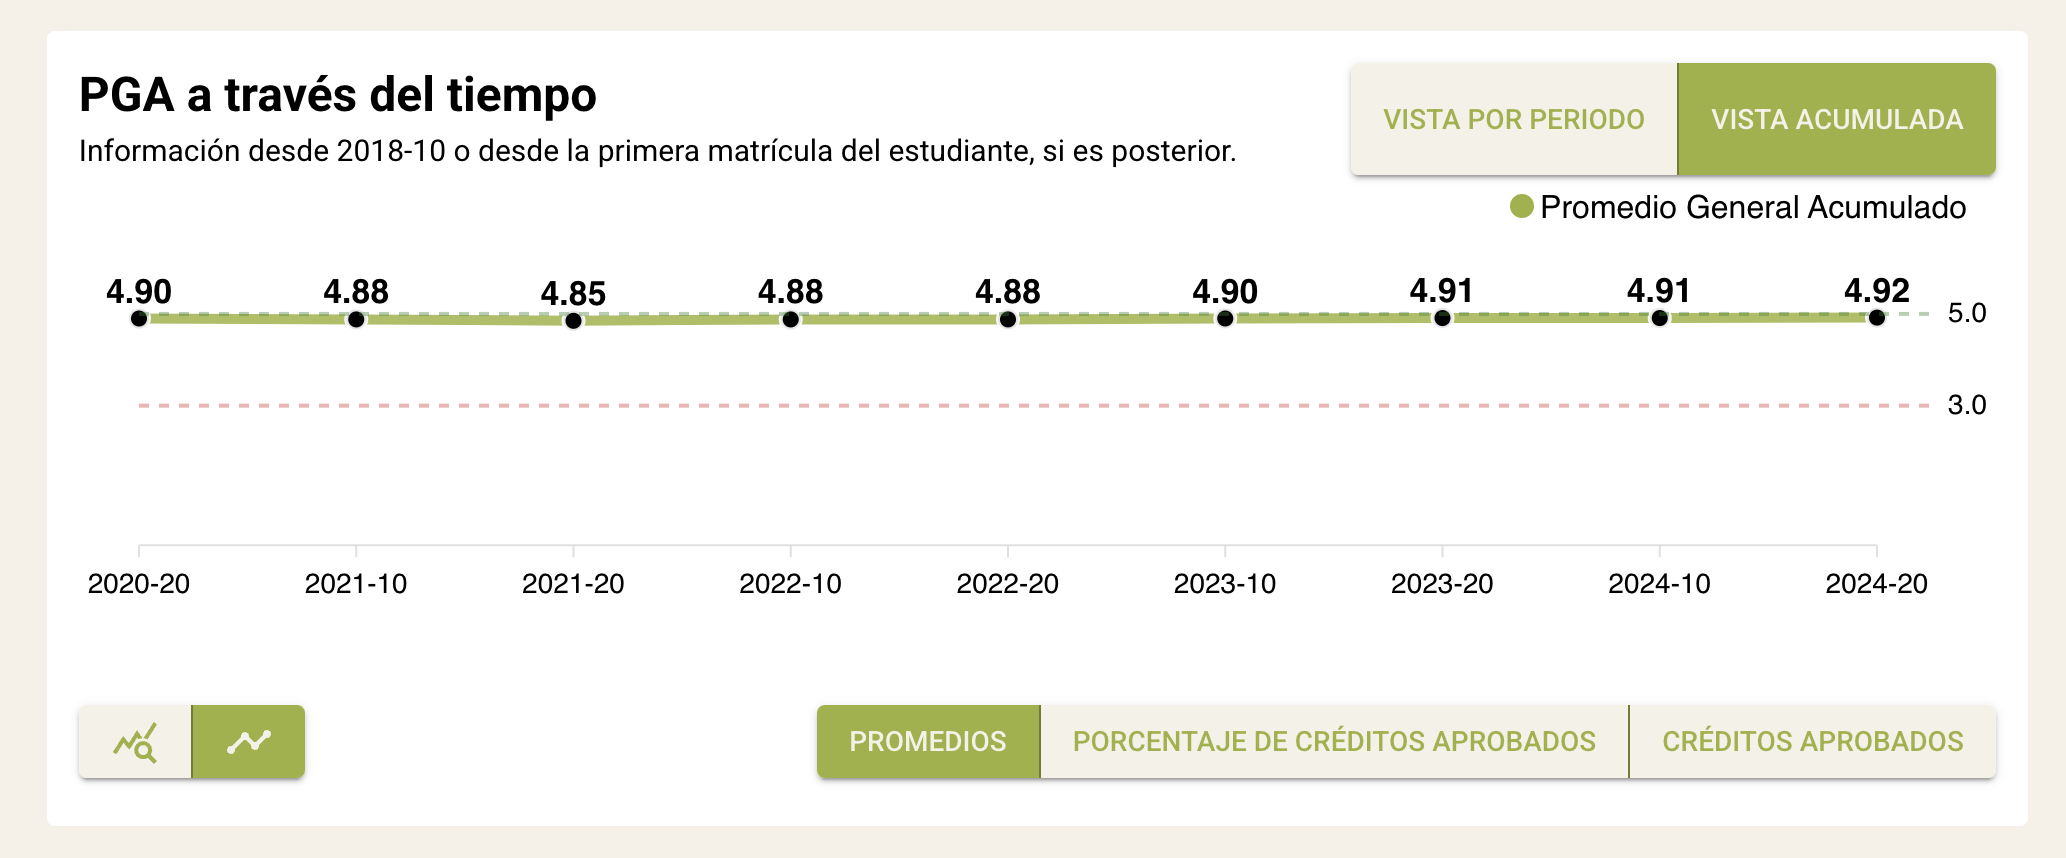
\includegraphics[width=0.8\textwidth]{assets/nes/pga_estandar.png}
		      \caption{Visualización de PGA a través del tiempo en escala estándar.}
		      \label{fig:pga_estandar}
	      \end{figure}

	\item \textbf{Promedios, Vista acumulada, Escala relativa.} Esta visualización transmite la misma información que la anterior y se titula igual. La diferencia radica en el enfoque que da a la información. Se modifica la escala de la gráfica para que el menor valor sea el PGA mínimo que el estudiante ha obtenido y el mayor valor sea el PGA máximo que ha alcanzado. Esto pone el énfasis en la variabilidad del PGA del alumno a lo largo del tiempo, permitiendo ver los periodos en los que mejoró o empeoró su rendimiento académico. Se presenta en la figura \ref{fig:pga_relativo}.

	      \begin{figure}[H]
		      \centering
		      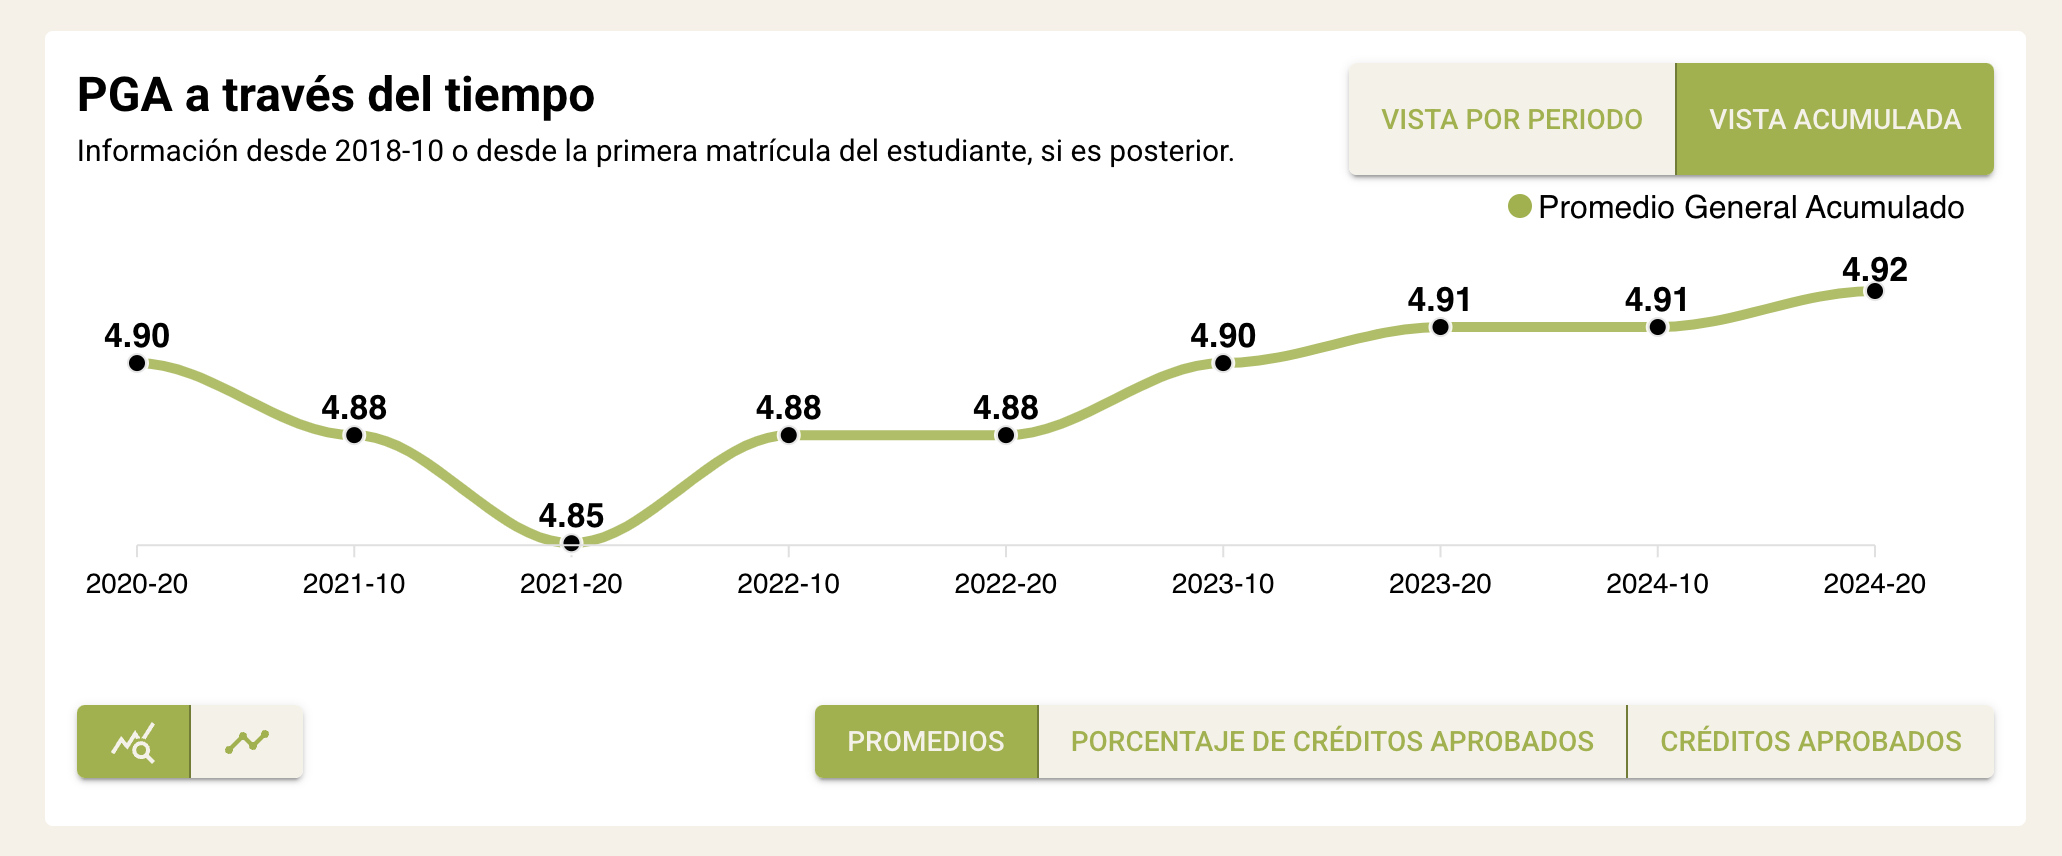
\includegraphics[width=0.8\textwidth]{assets/nes/pga_relativo.png}
		      \caption{Visualización de PGA a través del tiempo en escala relativa.}
		      \label{fig:pga_relativo}
	      \end{figure}

	\item \textbf{Promedios, Vista por periodo, Escala estándar.} Esta visualización se titula \say{Promedios semestrales a través del tiempo} y muestra los promedios semestrales que el estudiante ha obtenido a lo largo del tiempo. Cada punto de la gráfica representa el promedio semestral del alumno en un periodo académico específico. Se utiliza la misma escala estándar que en la visualización 1. Se presenta en la figura \ref{fig:promedios_estandar}.

	      \begin{figure}[H]
		      \centering
		      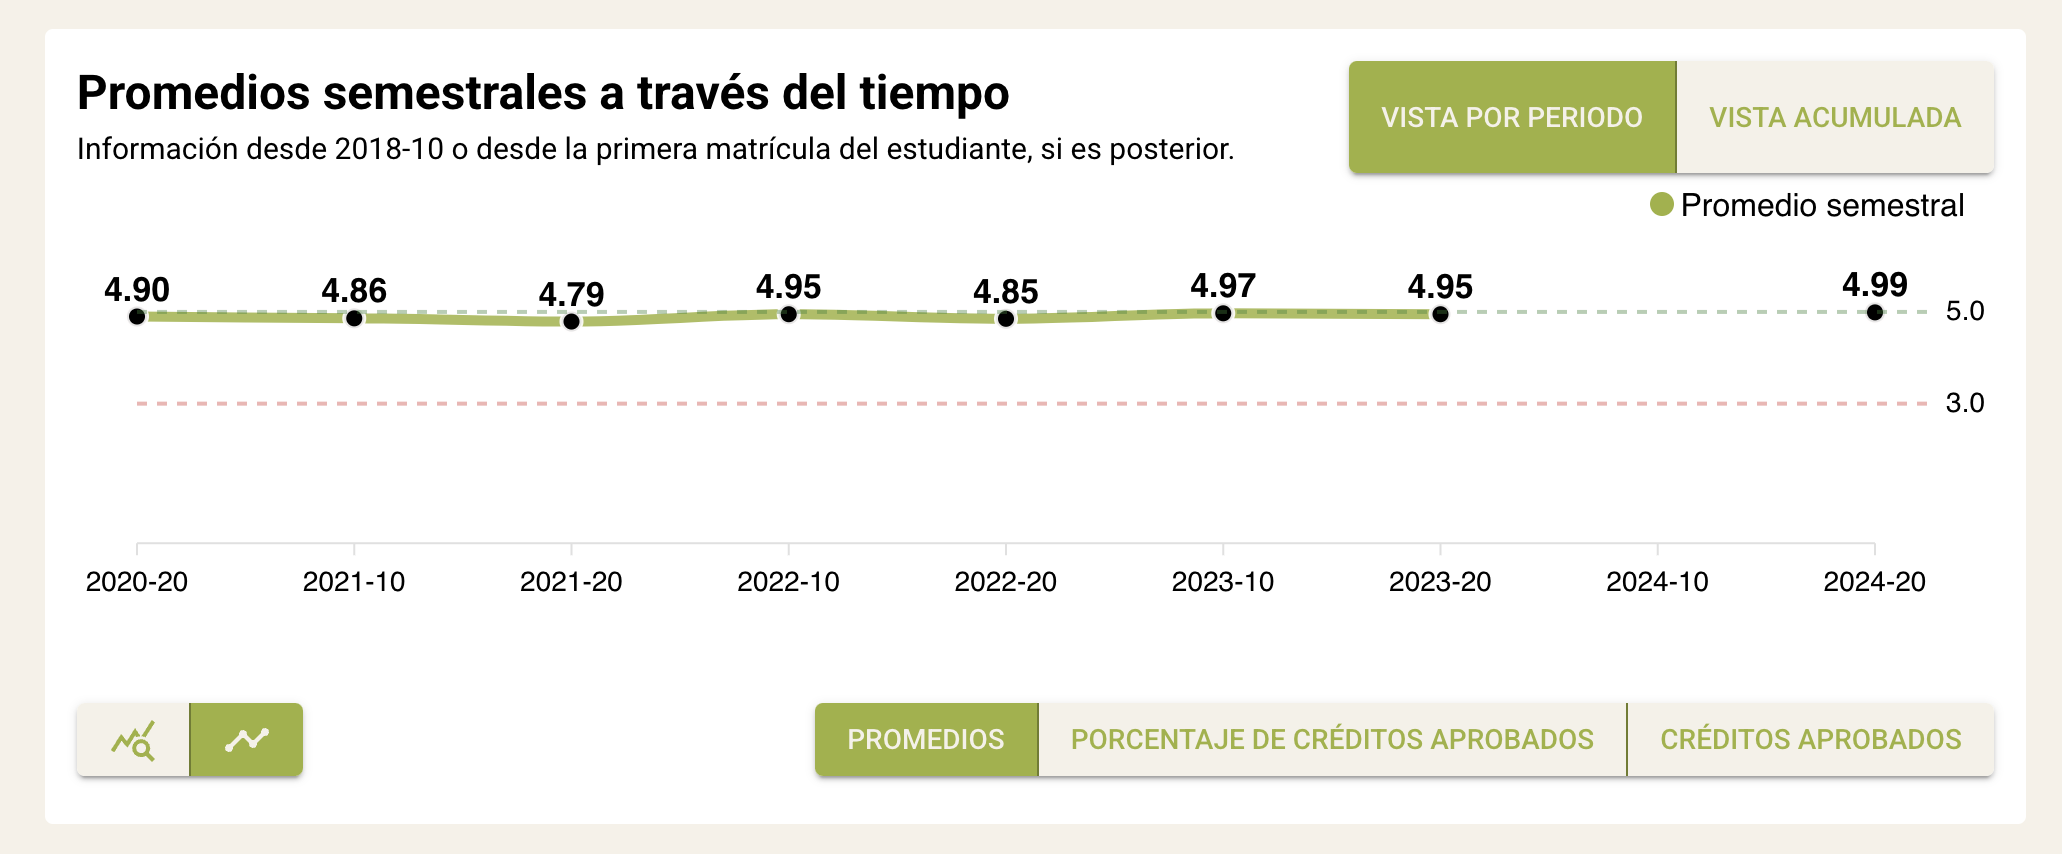
\includegraphics[width=0.8\textwidth]{assets/nes/promedios_estandar.png}
		      \caption{Visualización de promedios semestrales a través del tiempo en escala estándar.}
		      \label{fig:promedios_estandar}
	      \end{figure}

	      En la figura \ref{fig:promedios_estandar} resalta que hay un hueco en la gráfica. Esto puede suceder para alumnos que en un periodo académico determinado no tuvieron un promedio semestral numérico. Lo anterior puede deberse a varias causas; algunas de las más comunes son que el estudiante haya cursado un intercambio académico o una práctica académica, o que únicamente haya visto materias con calificación alfabética (por ejemplo: deportes o cursos de inglés). En estos casos, no se calcula un promedio semestral numérico, lo cual se ve reflejado en la gráfica mediante un salto. Ese espacio no se evidencia en la gráfica de la visualización 1 porque el PGA siempre es numérico, y si en un semestre no hay promedio semestral, el PGA se calcula con los promedios semestrales de los semestres anteriores.

	\item \textbf{Promedios, Vista por periodo, Escala relativa.} Similar a la visualización 2, esta visualización corresponde a la misma información de la visualización 3 pero pone el foco en el comportamiento del promedio semestral del estudiante a lo largo del tiempo. Se presenta en la figura \ref{fig:promedios_relativo}.

	      \begin{figure}[H]
		      \centering
		      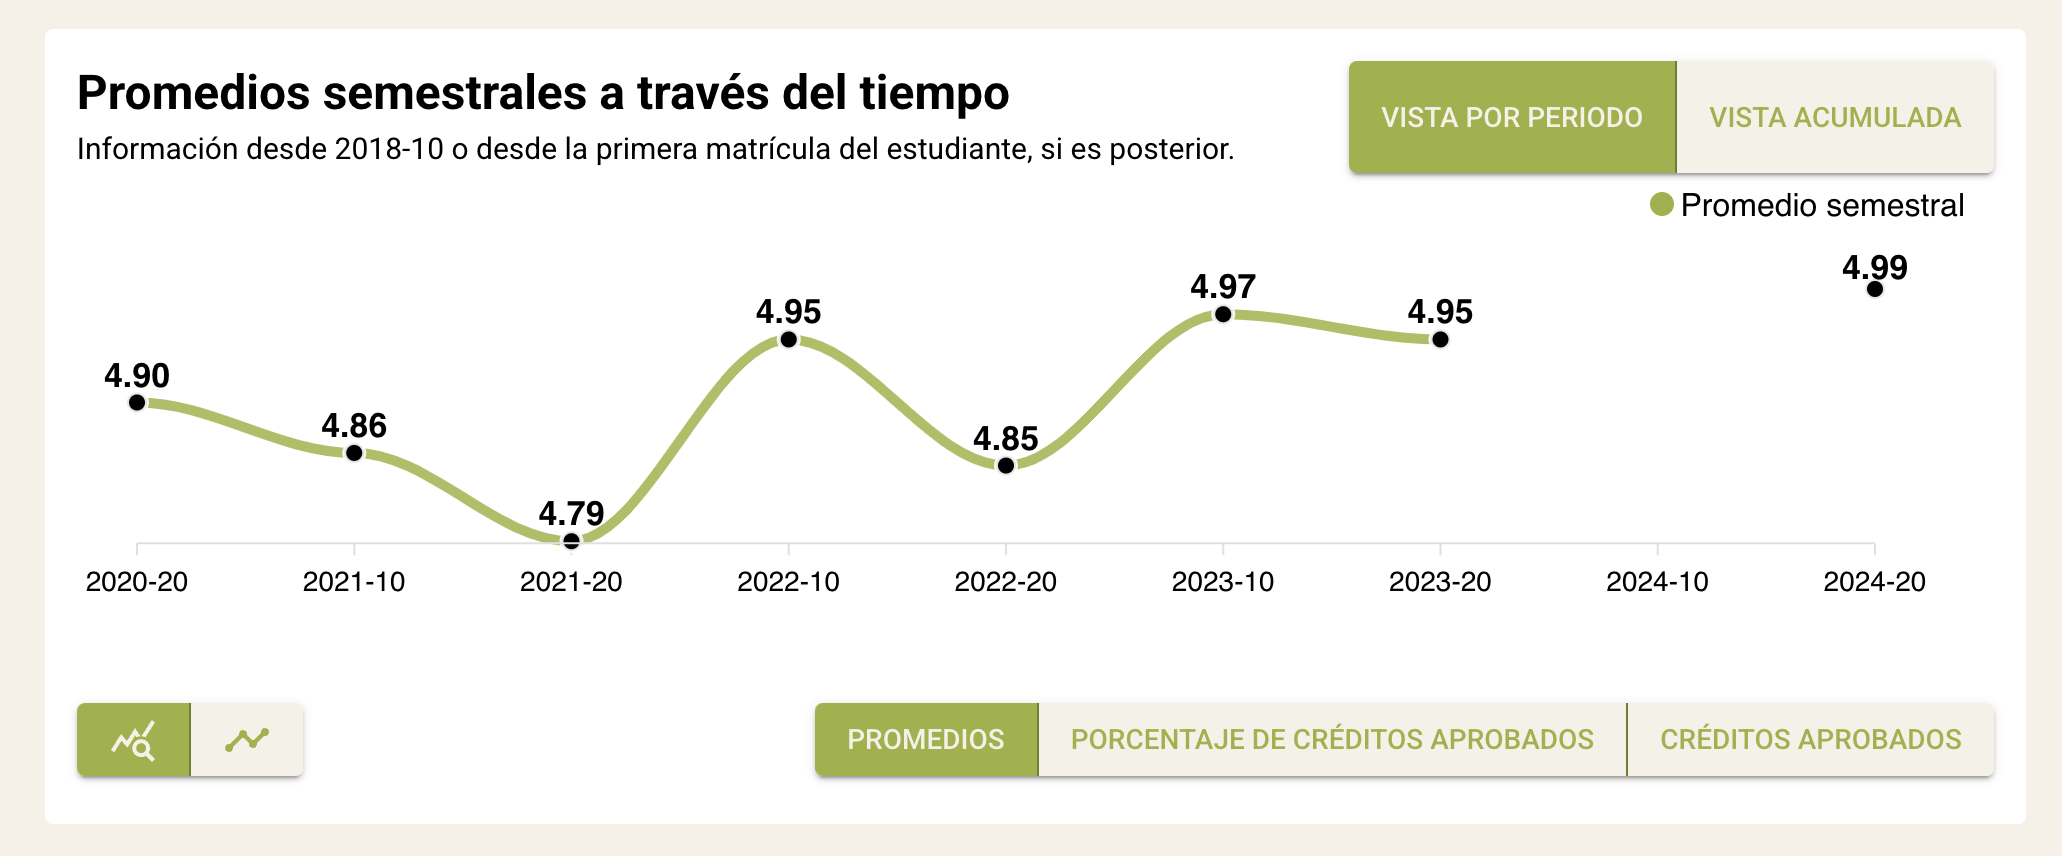
\includegraphics[width=0.8\textwidth]{assets/nes/promedios_relativo.png}
		      \caption{Visualización de promedios semestrales a través del tiempo en escala relativa.}
		      \label{fig:promedios_relativo}
	      \end{figure}

	\item \textbf{Porcentaje de Créditos Aprobados, Vista acumulada, Escala estándar.} Esta visualización se titula \say{Porcentaje acumulado de créditos aprobados} y muestra como ha cambiado el porcentaje de créditos aprobados por el alumno a lo largo del tiempo. En cada periodo, el porcentaje de créditos aprobados es acumulado, por lo cual contempla los periodos anteriores. Se utiliza una escala estándar con un mínimo de 0\% y un máximo de 100\%. Se trazan dos líneas de referencia, que son proporcionales a las trazadas en la visualización 1: la inferior se traza en rojo y corresponde al 60\% de los créditos aprobados; la superior se traza en verde y corresponde al 100\% de los créditos aprobados. Se presenta en la figura \ref{fig:porcentaje_estandar}.

	      \begin{figure}[H]
		      \centering
		      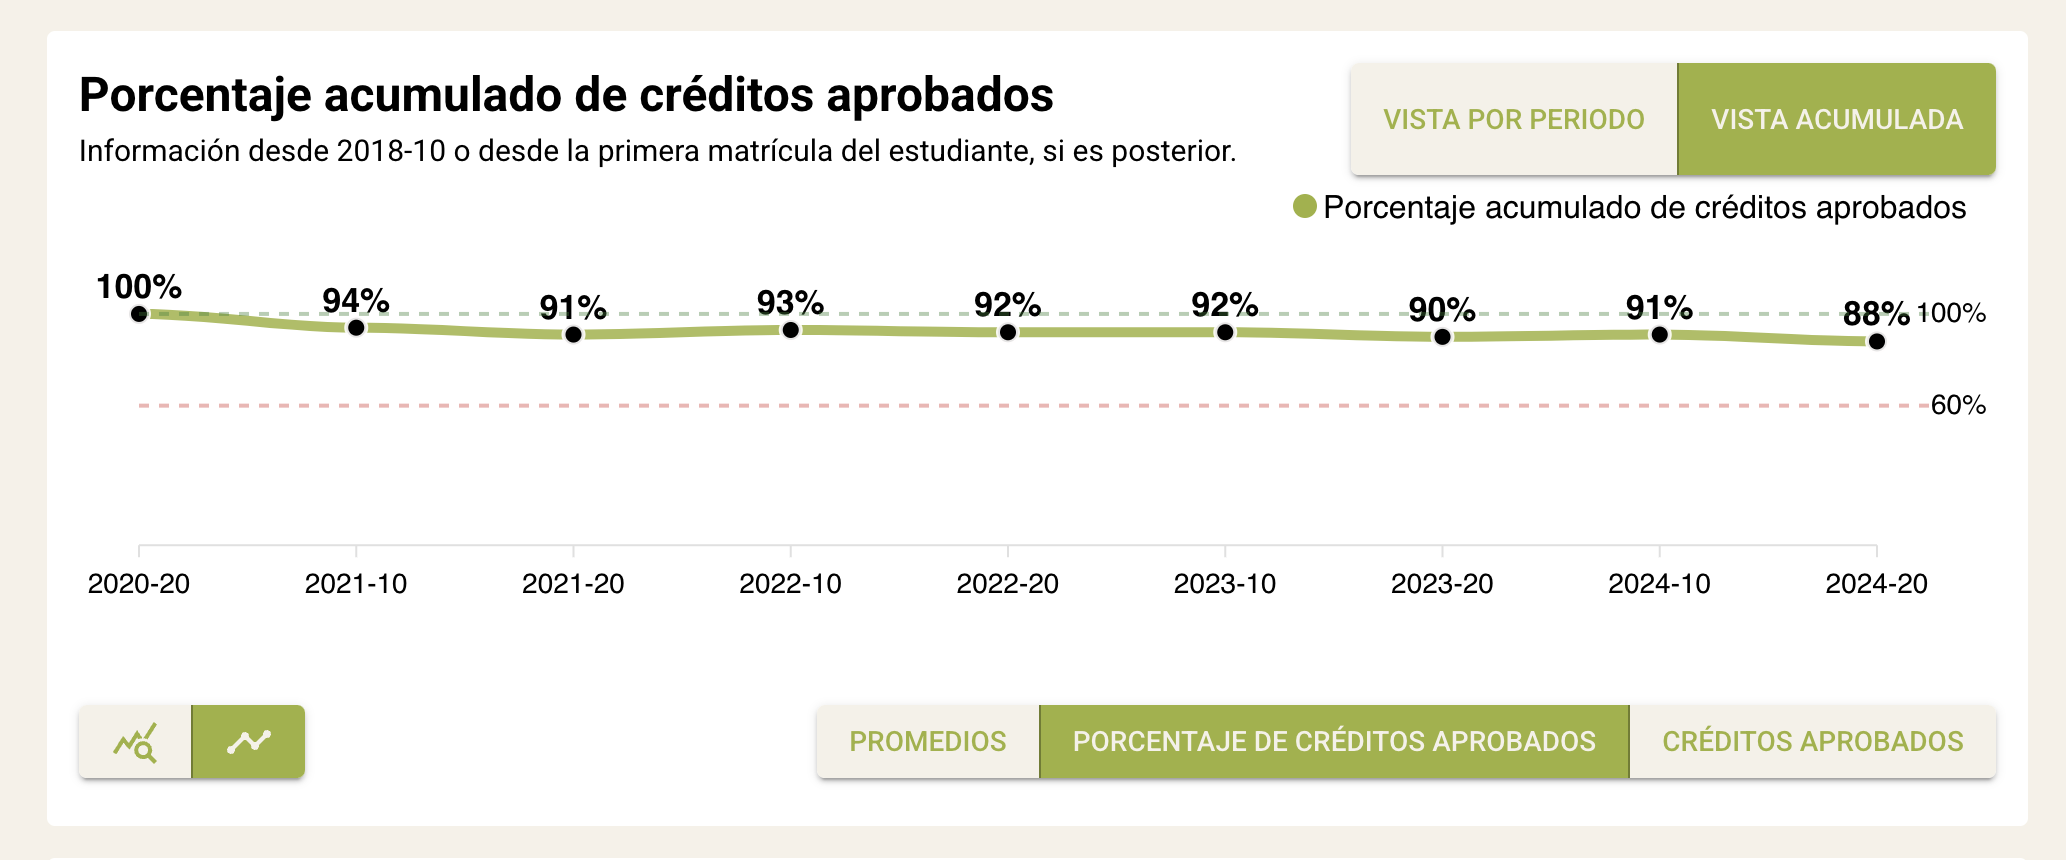
\includegraphics[width=0.8\textwidth]{assets/nes/porcentaje_estandar.png}
		      \caption{Visualización de porcentaje de créditos aprobados a través del tiempo en escala estándar.}
		      \label{fig:porcentaje_estandar}
	      \end{figure}

	\item \textbf{Porcentaje de Créditos Aprobados, Vista acumulada, Escala relativa.} Similar a la visualización 5, esta visualización pone el énfasis en la variabilidad del porcentaje de créditos aprobados del estudiante a lo largo del tiempo, en lugar de en los valores. Se presenta en la figura \ref{fig:porcentaje_relativo}.

	      \begin{figure}[H]
		      \centering
		      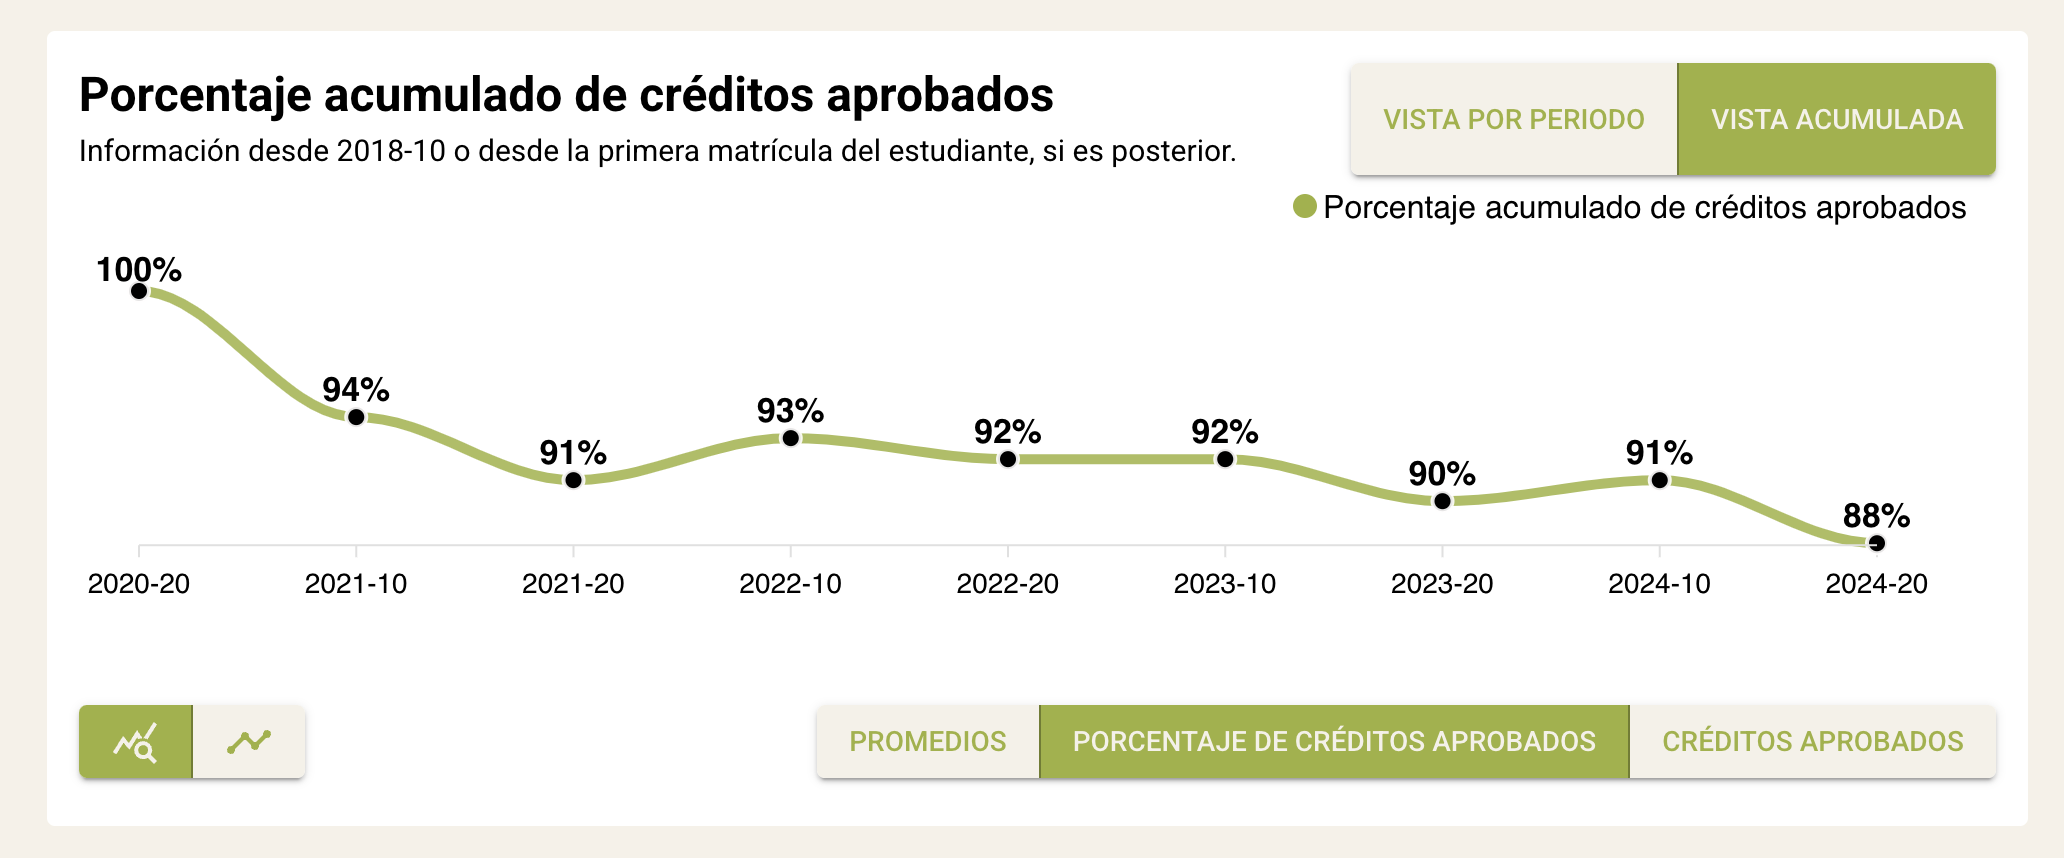
\includegraphics[width=0.8\textwidth]{assets/nes/porcentaje_relativo.png}
		      \caption{Visualización de porcentaje de créditos aprobados a través del tiempo en escala relativa.}
		      \label{fig:porcentaje_relativo}
	      \end{figure}

	\item \textbf{Porcentaje de Créditos Aprobados, Vista por periodo, Escala estándar.} Esta visualización se titula \say{Porcentaje de créditos aprobados por periodo} y muestra el porcentaje de créditos aprobados por el alumno en cada periodo académico, sin contemplar los periodos anteriores. Esto permite estudiar el desempeño del estudiante en cada periodo de forma independiente. Se utiliza la misma escala estándar que en la visualización 5. Se presenta en la figura \ref{fig:porcentaje_periodo_estandar}.

	      \begin{figure}[H]
		      \centering
		      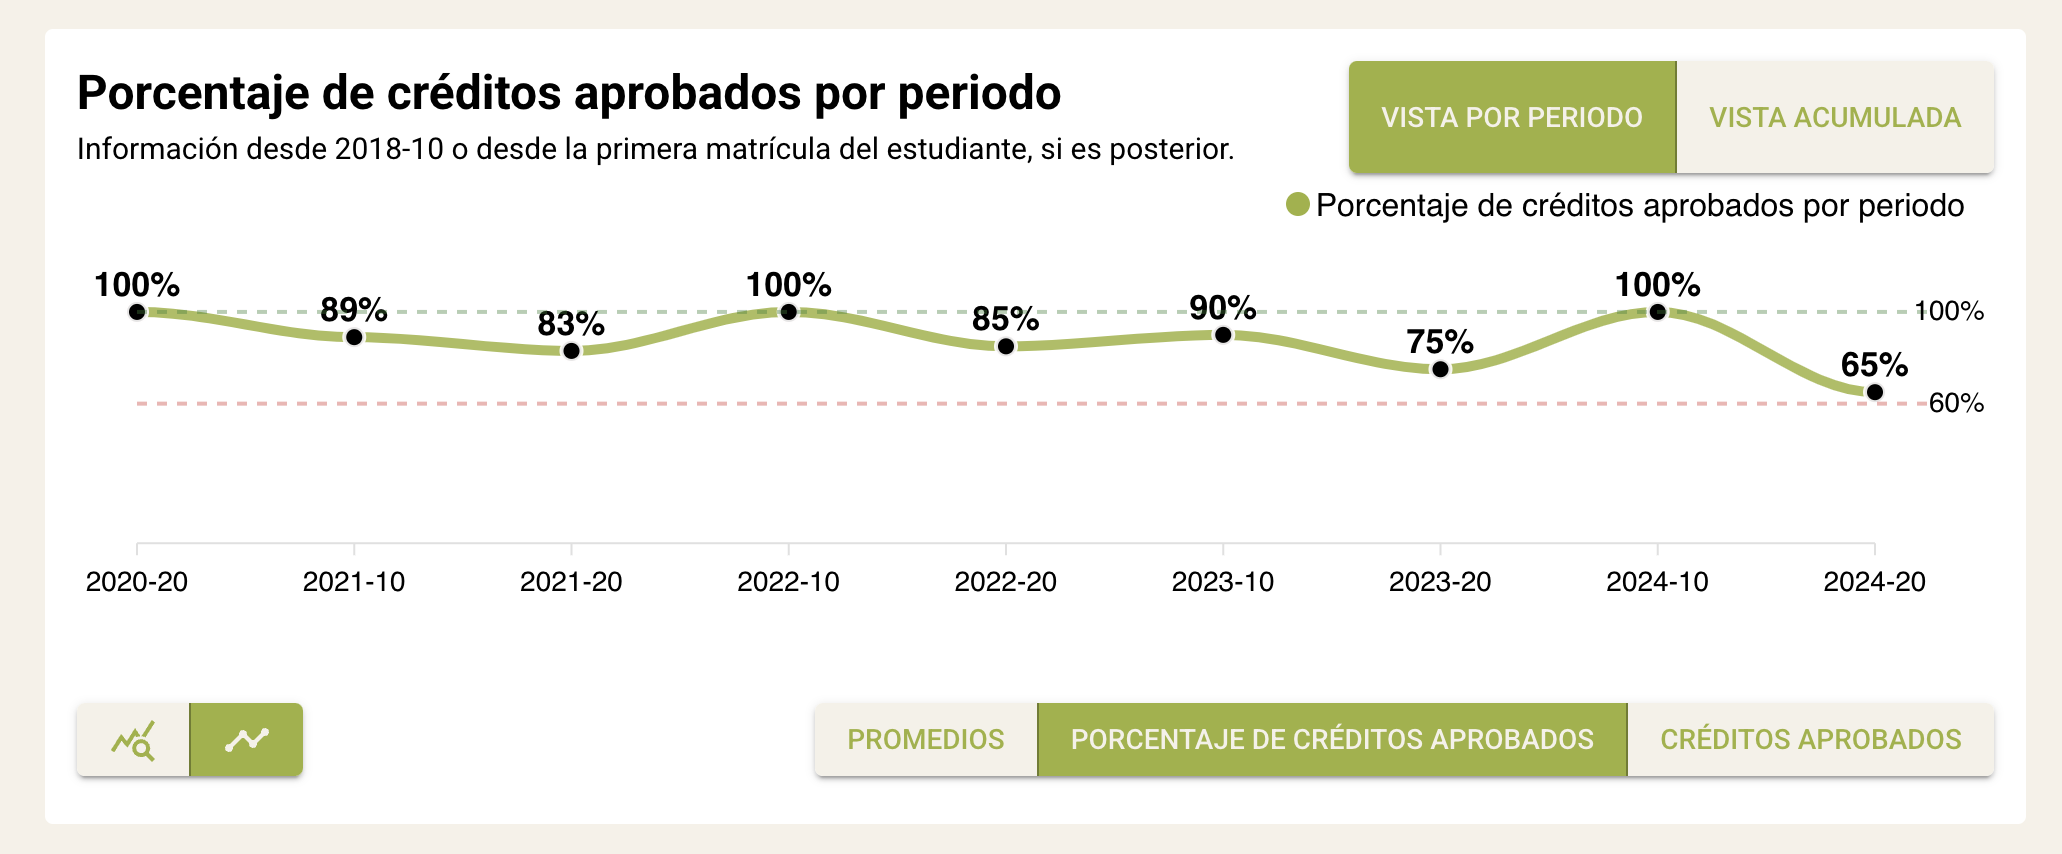
\includegraphics[width=0.8\textwidth]{assets/nes/porcentaje_periodo_estandar.png}
		      \caption{Visualización de porcentaje de créditos aprobados por periodo en escala estándar.}
		      \label{fig:porcentaje_periodo_estandar}
	      \end{figure}

	\item \textbf{Porcentaje de Créditos Aprobados, Vista por periodo, Escala relativa.} Similar a la visualización 7, esta visualización pone el énfasis en el comportamiento del porcentaje de créditos aprobados del estudiante en cada periodo académico. Se presenta en la figura \ref{fig:porcentaje_periodo_relativo}.

	      \begin{figure}[H]
		      \centering
		      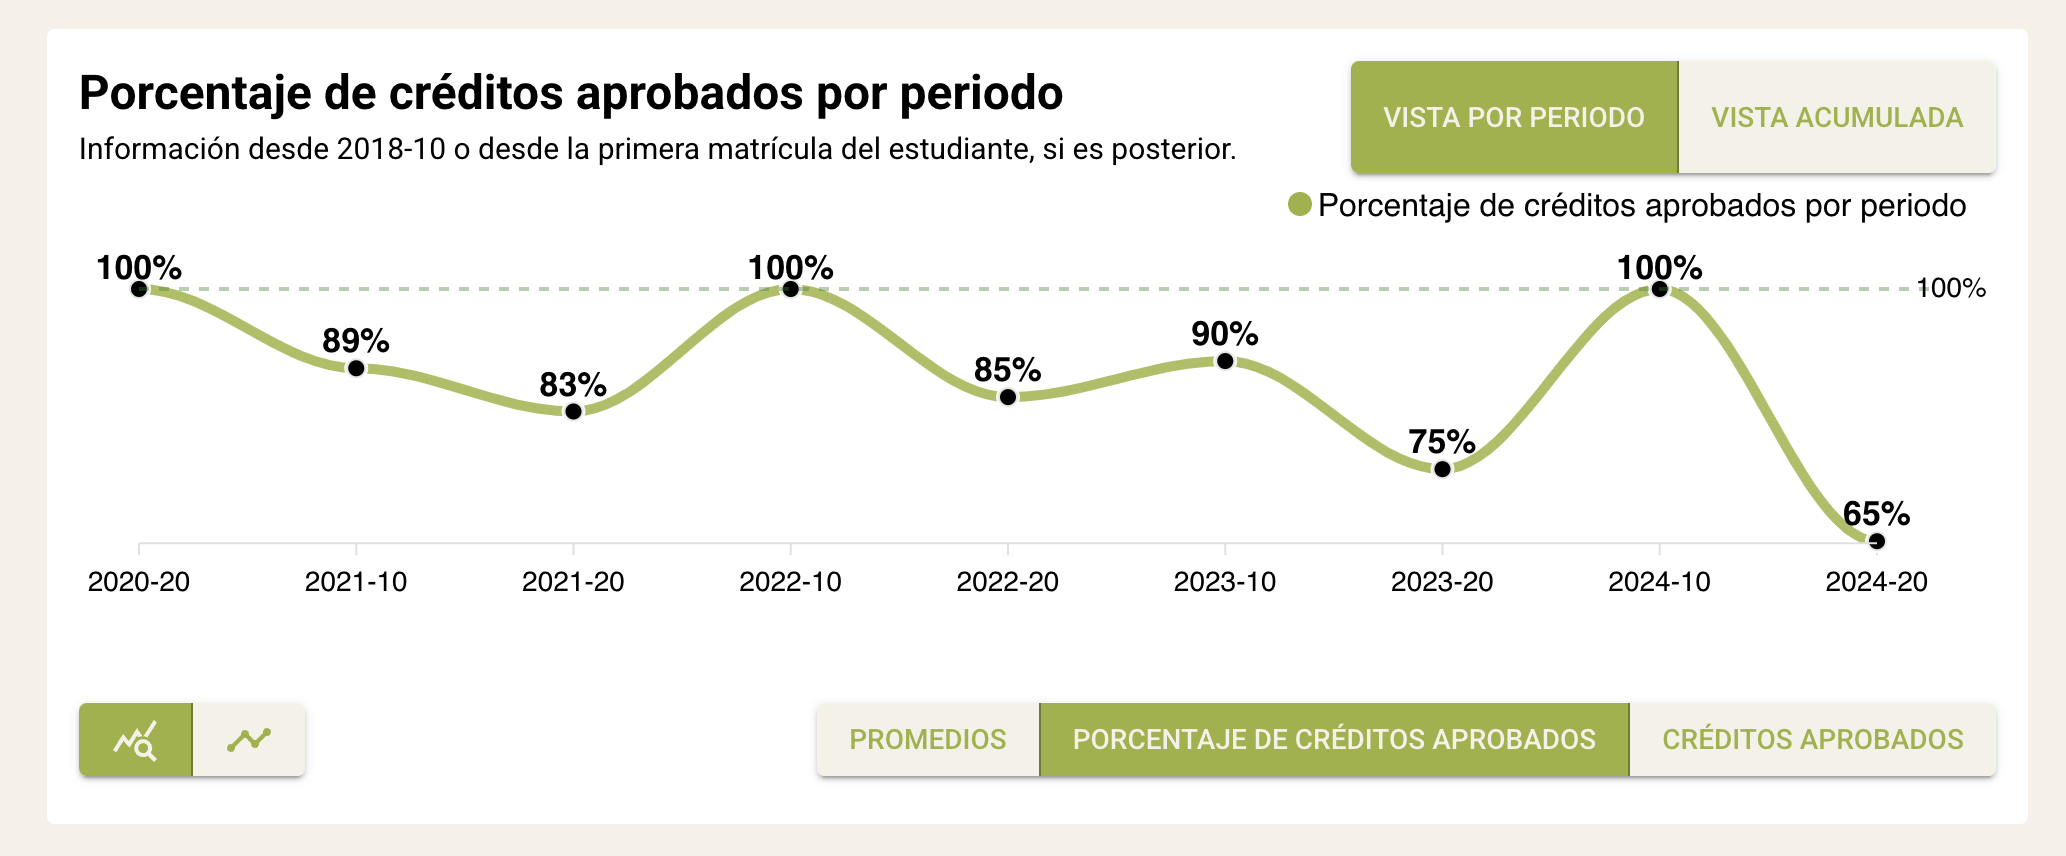
\includegraphics[width=0.8\textwidth]{assets/nes/porcentaje_periodo_relativo.png}
		      \caption{Visualización de porcentaje de créditos aprobados por periodo en escala relativa.}
		      \label{fig:porcentaje_periodo_relativo}
	      \end{figure}

	\item \textbf{Créditos Aprobados, Vista acumulada, Escala estándar.} Esta visualización se titula \say{Créditos aprobados acumulados} y muestra la cantidad de créditos aprobados por el estudiante a lo largo del tiempo. En cada periodo, los créditos aprobados son acumulados, por lo cual contempla los periodos anteriores. La escala estándar usa un mínimo de 0 créditos y utiliza como máximo el número de créditos aprobados por el alumno hasta la fecha. No se trazan líneas de referencia, pues no tiene sentido para esta gráfica, en la que un valor bajo en el total de créditos aprobados no indica un mal rendimiento sino simplemente una etapa temprana en la carrera del estudiante. Se presenta en la figura \ref{fig:creditos_estandar}.

	      \begin{figure}[H]
		      \centering
		      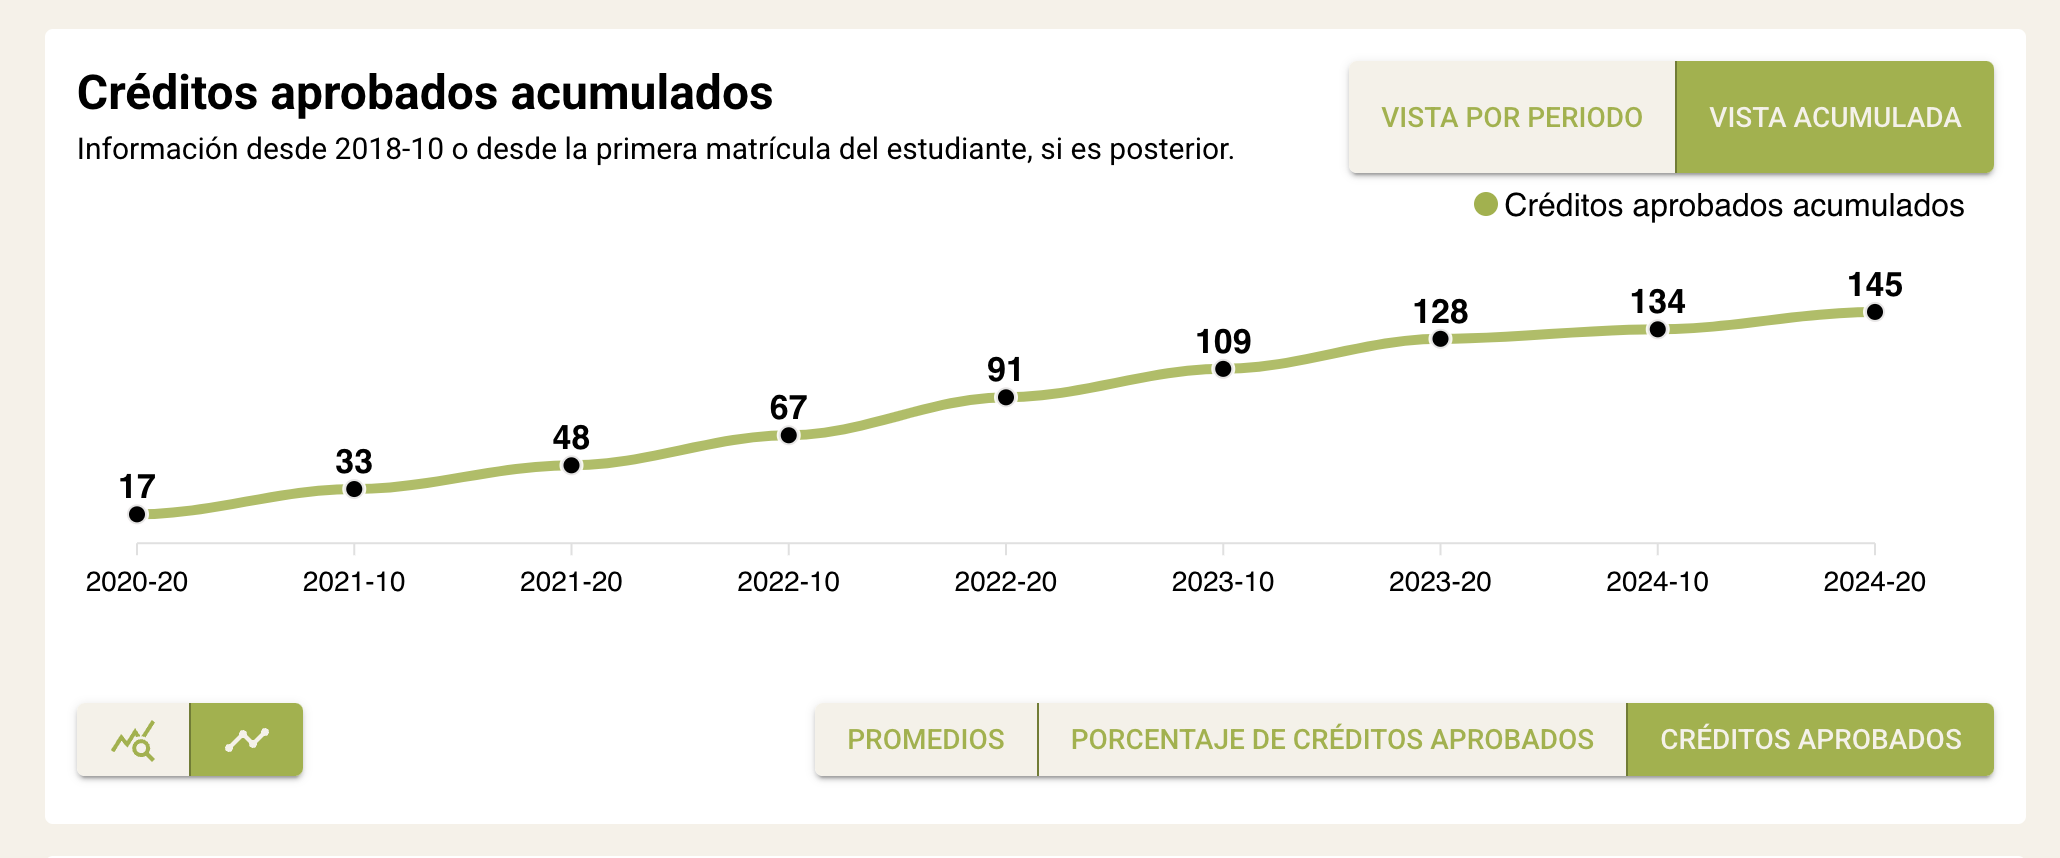
\includegraphics[width=0.8\textwidth]{assets/nes/creditos_estandar.png}
		      \caption{Visualización de créditos aprobados a través del tiempo en escala estándar.}
		      \label{fig:creditos_estandar}
	      \end{figure}

	\item \textbf{Créditos Aprobados, Vista acumulada, Escala relativa.} Esta visualización resulta muy similar a la anterior, con la única diferencia en que el valor mínimo es el número de créditos aprobados por el alumno en el periodo más temprano, en lugar de ser 0 créditos. Se presenta en la figura \ref{fig:creditos_relativo}.

	      \begin{figure}[H]
		      \centering
		      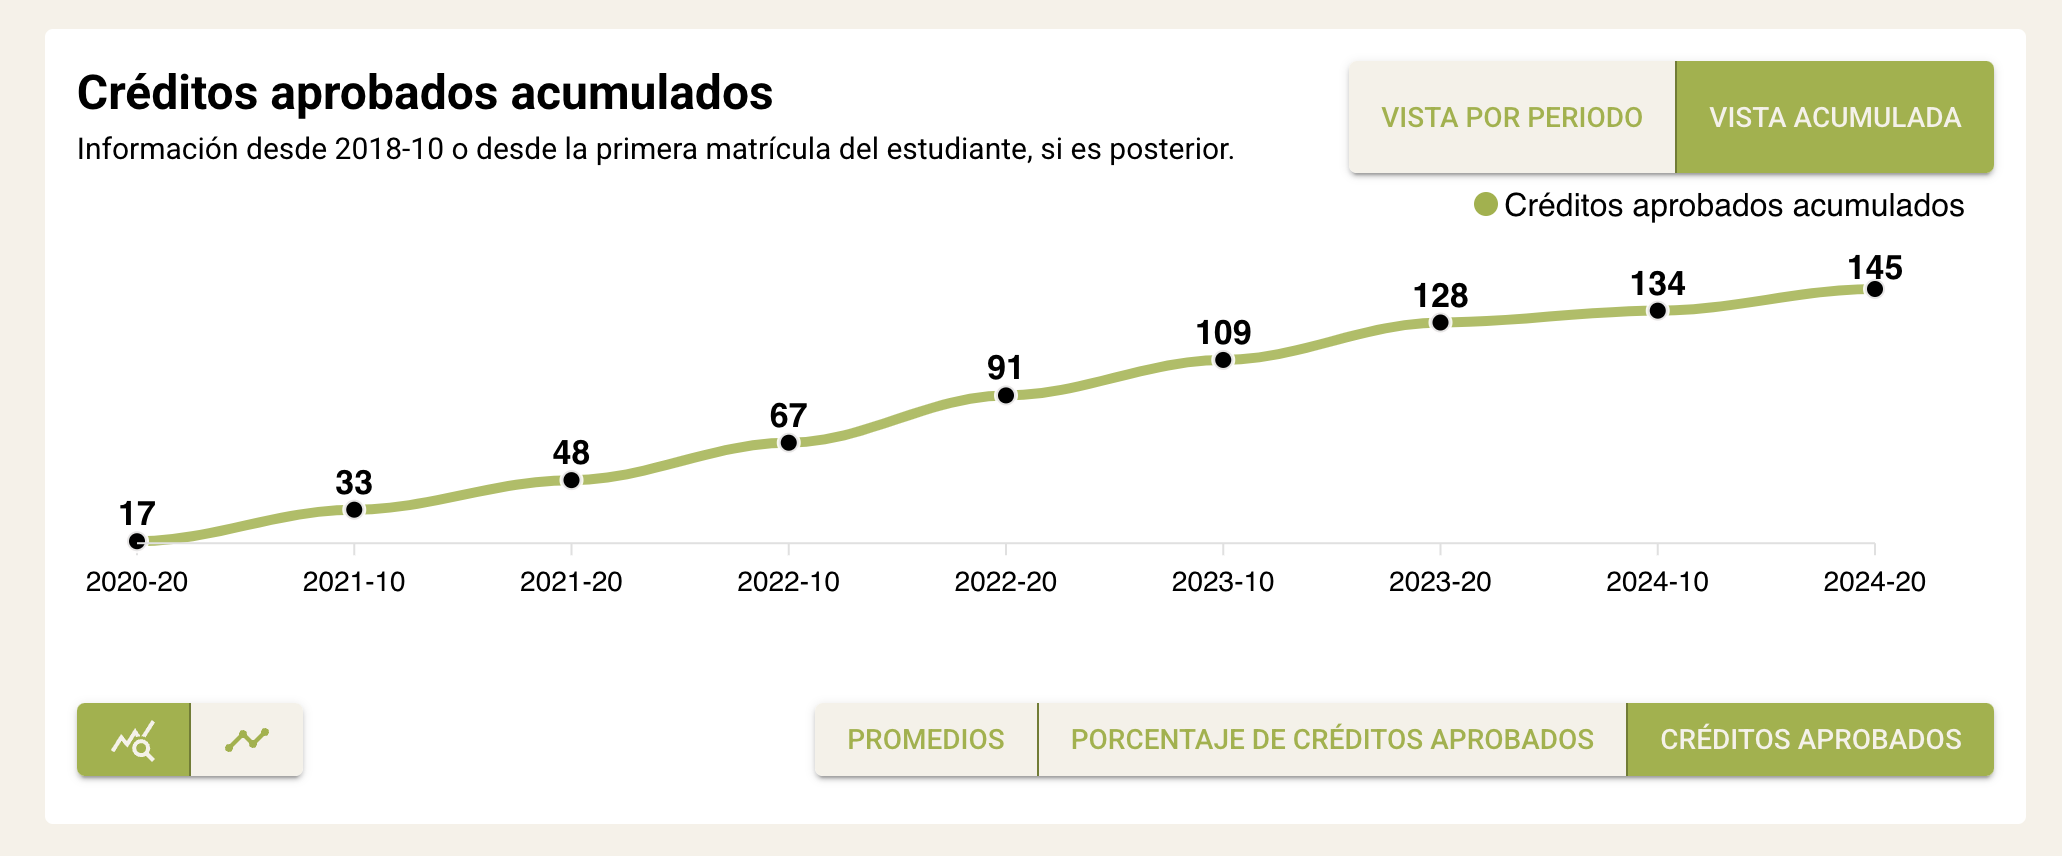
\includegraphics[width=0.8\textwidth]{assets/nes/creditos_relativo.png}
		      \caption{Visualización de créditos aprobados a través del tiempo en escala relativa.}
		      \label{fig:creditos_relativo}
	      \end{figure}

	\item \textbf{Créditos Aprobados, Vista por periodo, Escala estándar.} Esta visualización se titula \say{Créditos aprobados por periodo} y muestra la cantidad de créditos aprobados por el estudiante en cada periodo académico, sin contemplar los periodos anteriores. La escala estándar usa un mínimo de 0 créditos y un máximo que depende del número de créditos aprobados en el periodo con más créditos aprobados. Se traza una línea de referencia, a la altura de los 11 créditos, que no necesariamente tiene connotaciones negativas, teniendo en cuenta que el alumno puede haber cursado matrículas parciales. Se presenta en la figura \ref{fig:creditos_periodo_estandar}.

	      \begin{figure}[H]
		      \centering
		      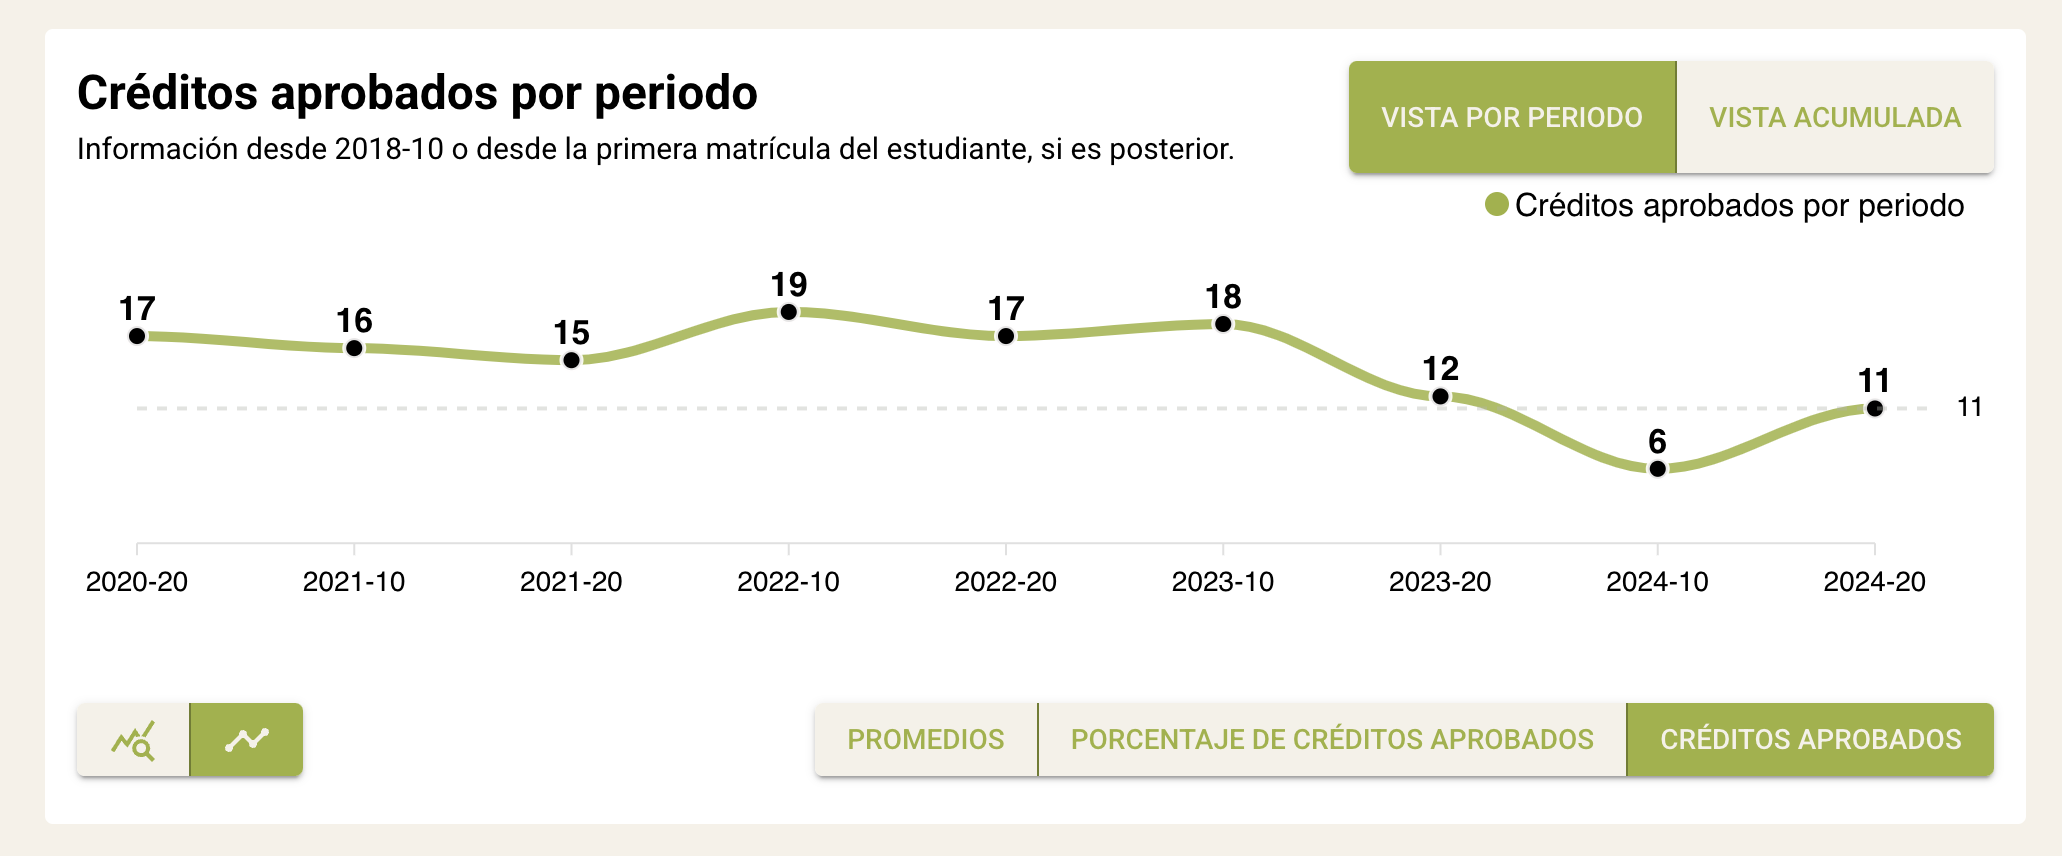
\includegraphics[width=0.8\textwidth]{assets/nes/creditos_periodo_estandar.png}
		      \caption{Visualización de créditos aprobados por periodo en escala estándar.}
		      \label{fig:creditos_periodo_estandar}
	      \end{figure}

	\item \textbf{Créditos Aprobados, Vista por periodo, Escala relativa.} Esta última visualización presenta la misma información que la visualización 11, pero pone el énfasis en el comportamiento del número de créditos aprobados por el estudiante en cada periodo académico. Se presenta en la figura \ref{fig:creditos_periodo_relativo}.

	      \begin{figure}[H]
		      \centering
		      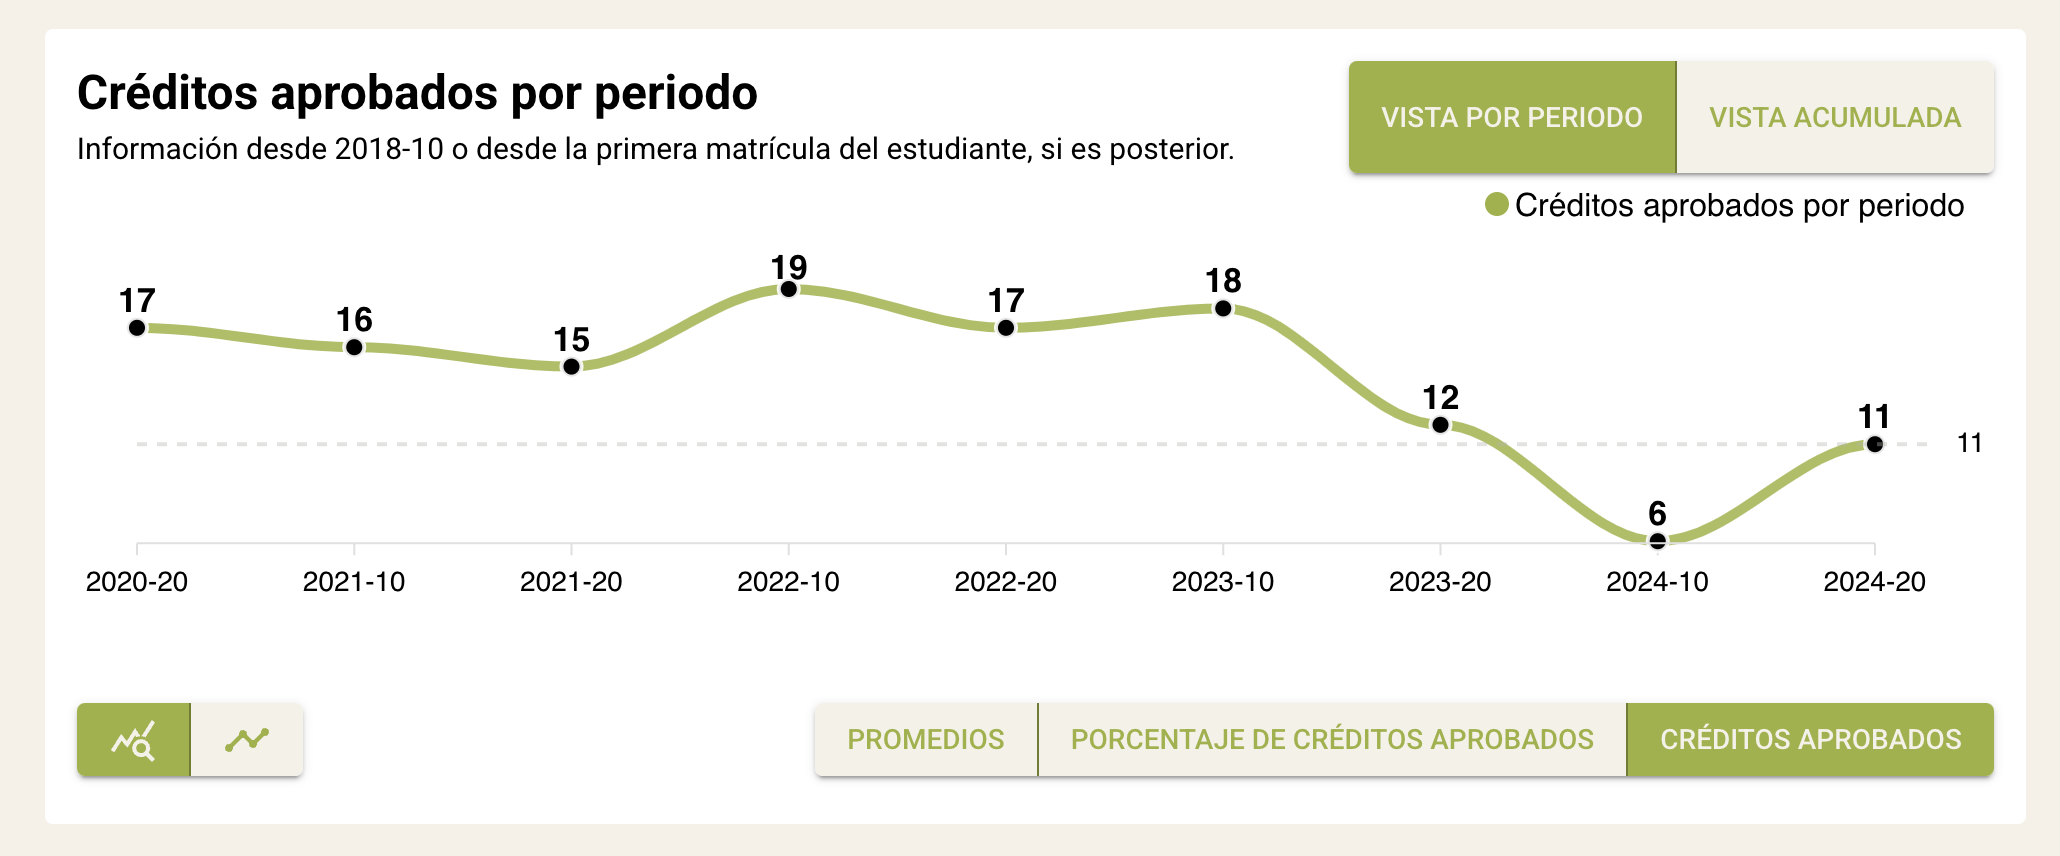
\includegraphics[width=0.8\textwidth]{assets/nes/creditos_periodo_relativo.png}
		      \caption{Visualización de créditos aprobados por periodo en escala relativa.}
		      \label{fig:creditos_periodo_relativo}
	      \end{figure}
\end{enumerate}

\paragraph{Tabla de créditos inscritos} La tabla de créditos inscritos es el siguiente componente de la pestaña de Desempeño. Se muestra en la figura \ref{fig:tabla_creditos}. La primera fila de la tabla proporciona un resumen del total de créditos inscritos por el alumno, clasificándolos en \textit{aprobados}, \textit{reprobados}, \textit{retirados}, \textit{incompletos} y \textit{pendientes}. La segunda fila de la tabla permite al usuario visualizar ese desglose de los créditos inscritos pero con relación a un área de conocimiento específica, que el usuario selecciona de un menú desplegable. Por ejemplo, para los estudiantes de ingeniería, se puede seleccionar las áreas de matemáticas, física o su ingeniería específica. La tabla se actualiza automáticamente al seleccionar un área de conocimiento distinta. Como interacción adicional, la tabla incluye la posibilidad de alternar los valores desplegados como  cantidad absoluta de créditos o como porcentaje del total de créditos inscritos, facilitando el análisis de los datos por parte del usuario.

\begin{figure}[H]
	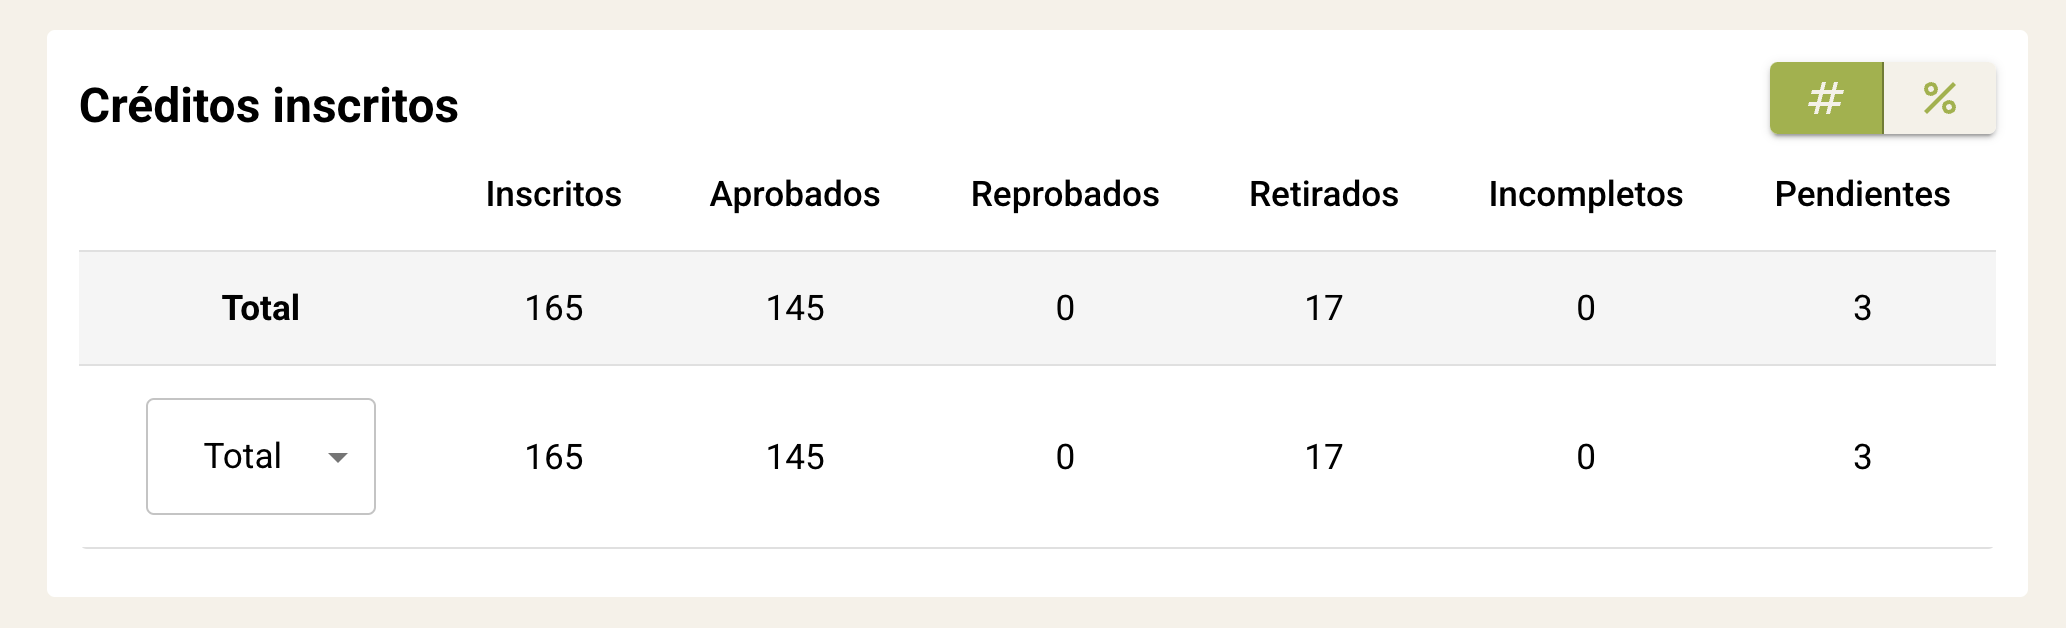
\includegraphics[width=\textwidth]{assets/nes/tabla_creditos.png}
	\caption{Tabla de créditos inscritos.}
	\label{fig:tabla_creditos}
\end{figure}

\paragraph{Gráfica de créditos por periodo} Tras lo anterior, aparece la gráfica de créditos por periodo, exhibida en la figura \ref{fig:grafica_creditos}. Esta gráfica desglosa el número de créditos aprobados, retirados y reprobados en cada periodo académico. Traza una curva para cada uno, pintando los créditos aprobados en verde, los retirados en azul y los reprobados en rojo. Esta gráfica, al igual que la primera, también cuenta con múltiples representaciones. Sin embargo, en ese caso es más sensato explicar las posibles interacciones de la gráfica, sin necesidad de listar las doce visualizaciones posibles.

\begin{figure}[H]
	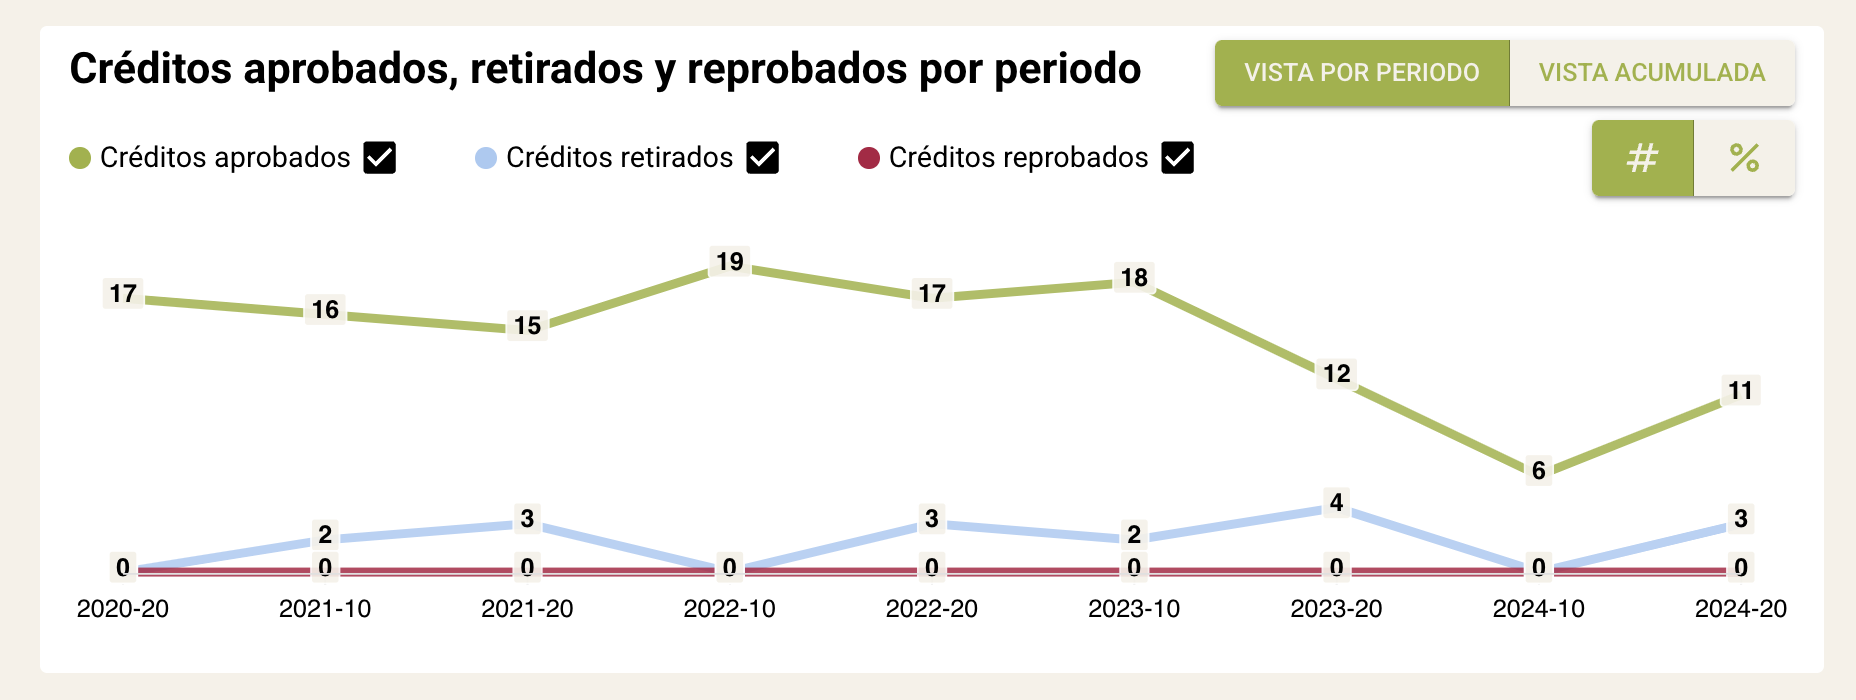
\includegraphics[width=\textwidth]{assets/nes/grafica_creditos.png}
	\caption{Gráfica de créditos por periodo.}
	\label{fig:grafica_creditos}
\end{figure}

\begin{itemize}
	\item \textbf{Esconder alguna, dos o todas las curvas.} La gráfica permite al usuario seleccionar cuáles curvas desea visualizar. Por defecto, se muestran todas las curvas, pero el usuario puede deseleccionar alguna o todas las curvas para enfocarse en una sola o en contrastar dos curvas. Esto resulta útil para reducir el ruido en análisis específicos, como comparar el número de créditos aprobados con el número de créditos reprobados, determinar el comportamiento de específicamente los créditos retirados, entre otros. En la figura \ref{fig:creditos_retirados} se muestra un ejemplo en el que se han deseleccionado las curvas de créditos aprobados y reprobados, dejando solo la curva de créditos retirados.

	      \begin{figure}[H]
		      \centering
		      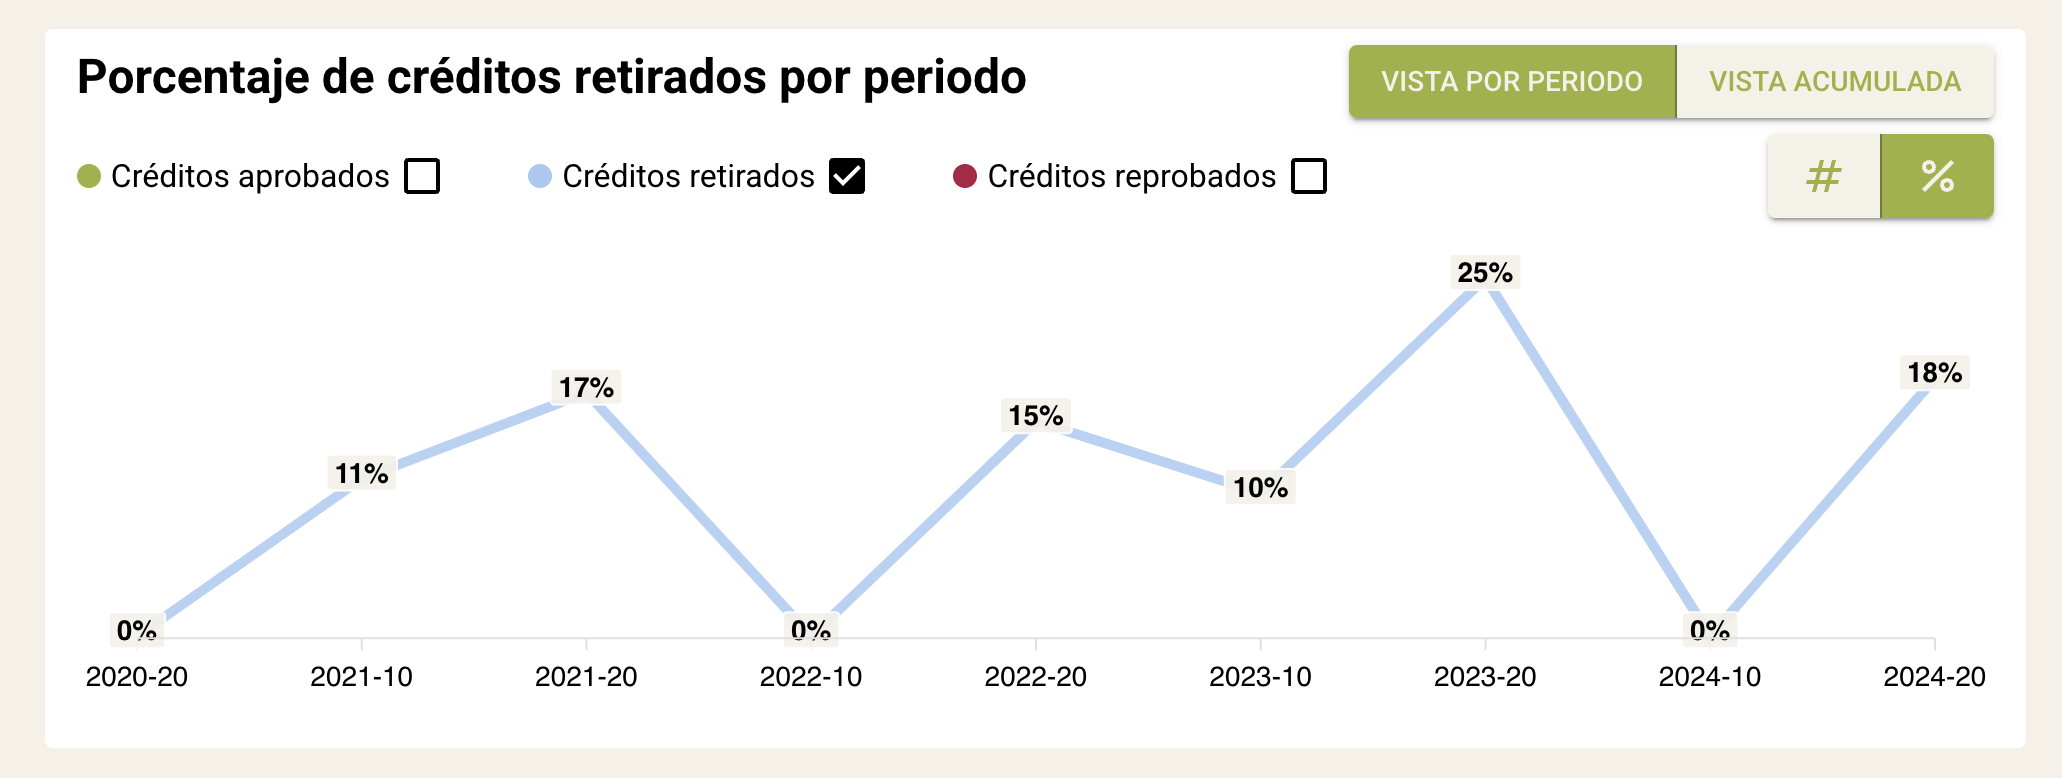
\includegraphics[width=0.8\textwidth]{assets/nes/creditos_retirados.png}
		      \caption{Gráfica de créditos por periodo con solo la curva de créditos retirados.}
		      \label{fig:creditos_retirados}
	      \end{figure}

	\item \textbf{Vista por periodo o acumulada.} Al igual que la gráfica central, esta de créditos por periodo permite al usuario alternar entre una vista por periodo y una vista acumulada. La vista por periodo muestra el comportamiento de los créditos aprobados, retirados y reprobados en cada periodo académico, mientras que la vista acumulada muestra la evolución de esos créditos a lo largo del tiempo. La vista acumulada es particularmente útil para ver cómo el número de créditos aprobados, retirados y reprobados ha cambiado a lo largo de la carrera del estudiante. La figura \ref{fig:creditos_acumulados} muestra un ejemplo de la gráfica de créditos por periodo en vista acumulada.

	      \begin{figure}[H]
		      \centering
		      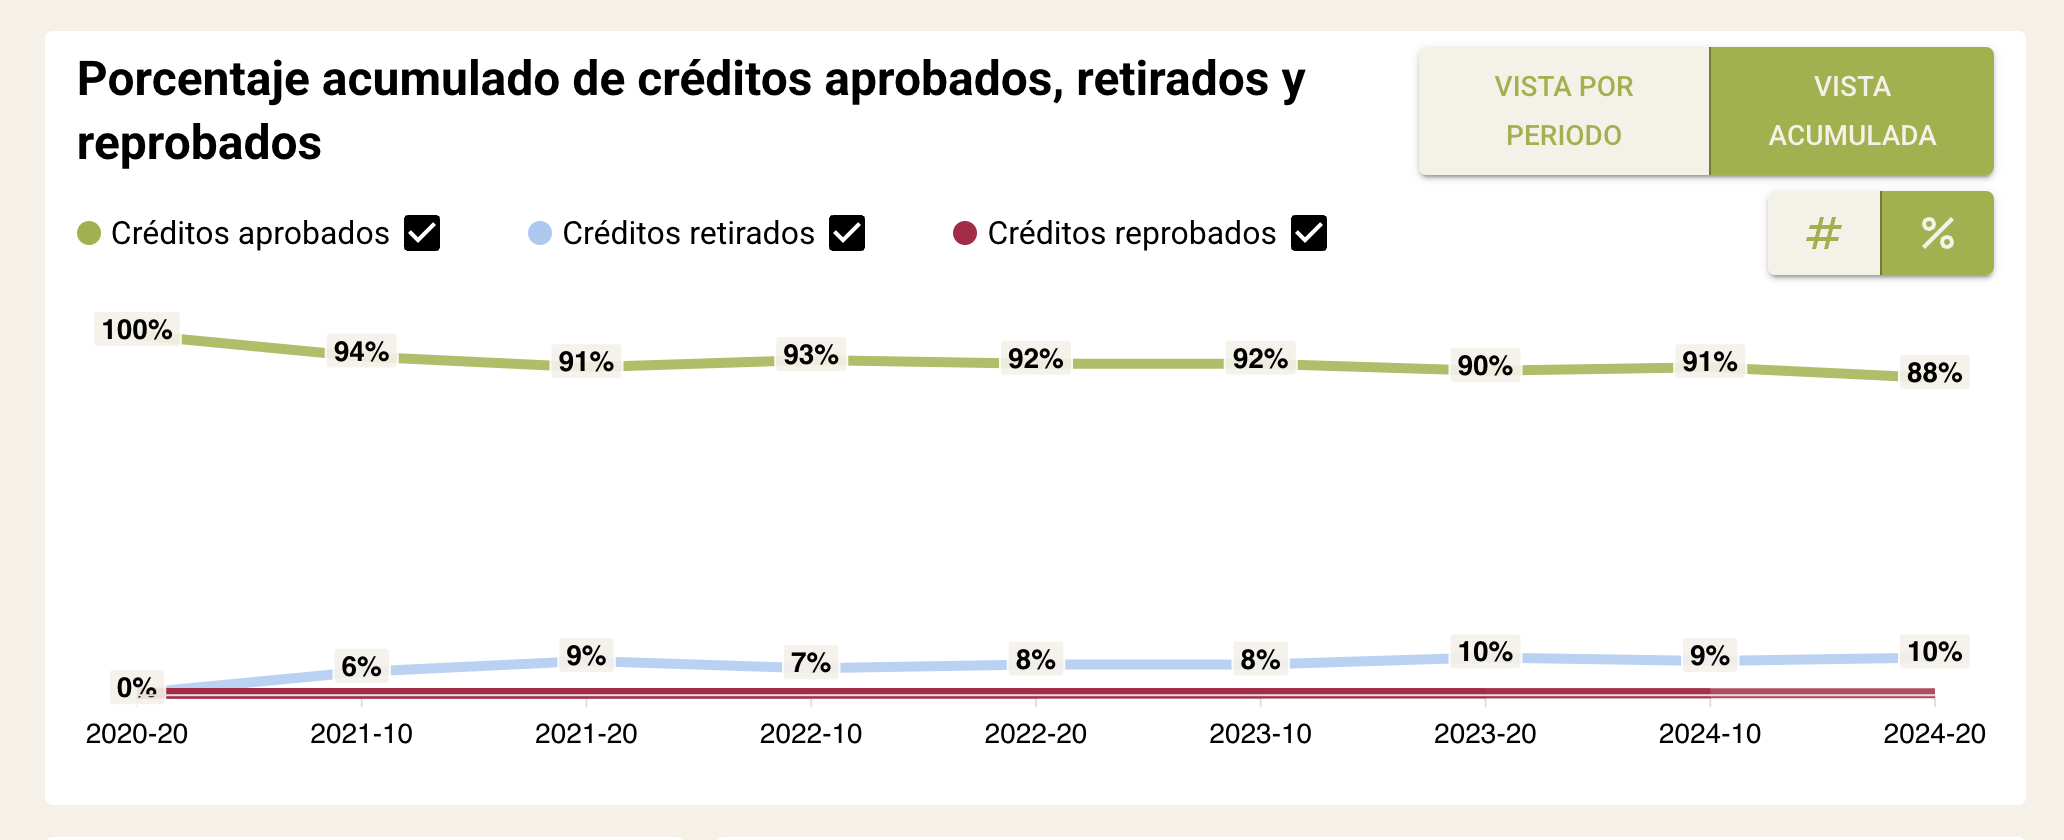
\includegraphics[width=0.8\textwidth]{assets/nes/creditos_acumulados.png}
		      \caption{Gráfica de créditos por periodo en vista acumulada.}
		      \label{fig:creditos_acumulados}
	      \end{figure}

	\item \textbf{Vista porcentual o absoluta.} Al igual que la tabla de créditos inscritos, la gráfica de créditos por periodo permite al usuario alternar entre una vista porcentual y una vista absoluta. La vista porcentual es particularmente útil para comparar el comportamiento de los créditos aprobados, retirados y reprobados en cada periodo académico, independientemente del número total de créditos inscritos. Las figuras \ref{fig:creditos_retirados} y \ref{fig:creditos_acumulados} constituyen ejemplos de la gráfica de créditos por en vista porcentual, mientras que la figura \ref{fig:grafica_creditos} muestra la gráfica en vista absoluta.
\end{itemize}

\paragraph{Condiciones académicas} En la parte inferior izquierda de la pestaña de Desempeño, se presenta la cantidad de suspensiones académicas, pruebas académicas, pruebas de reingreso e incompletos totales que el estudiante ha tenido a lo largo de su carrera. Se muestra en la figura \ref{fig:condiciones_academicas}. Es un componente simple, al que la interactividad no le agregaría valor, pero constituye una pieza de información crucial para el usuario, sobretodo si el conteo de alguno de esos indicadores es mayor a cero.

\begin{figure}[H]
	\centering
	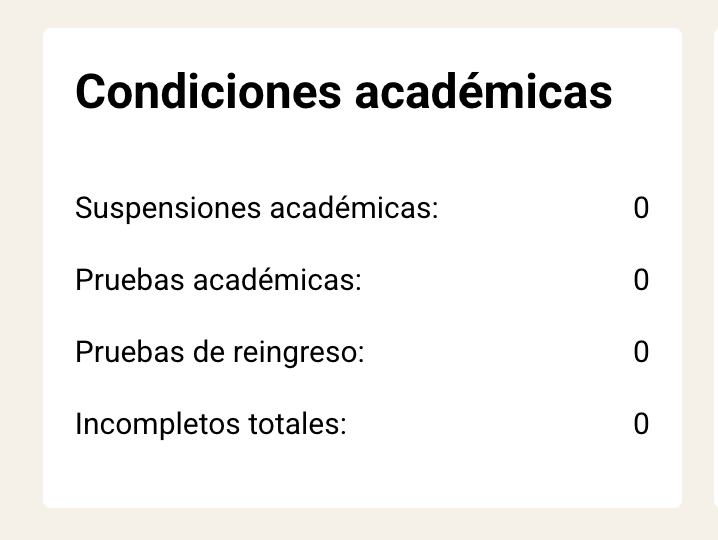
\includegraphics[width=0.4\textwidth]{assets/nes/condiciones_academicas.png}
	\caption{Condiciones académicas.}
	\label{fig:condiciones_academicas}
\end{figure}

\paragraph{Resultados del ICFES} En la parte inferior derecha de la pestaña, se resume el desempeño del estudiante en el examen de estado Saber Pro, como se puede evidenciar en la figura \ref{fig:icfes}. Se presenta el puntaje global del examen, así como los puntajes específicos obtenidos en cada una de las áreas del examen. Se presenta un gráfico de radar que ilustra los puntajes de cada área y permite reconocer las fortalezas y debilidades del alumno un solo vistazo. Este gráfico es interactivo y permite al usuario visualizar los puntajes de cada área al pasar el cursor sobre el gráfico. En esa tarjeta se incluye también el nombre de la institución que otorgó el diploma de bachiller al estudiante en cuestión.

\begin{figure}[H]
	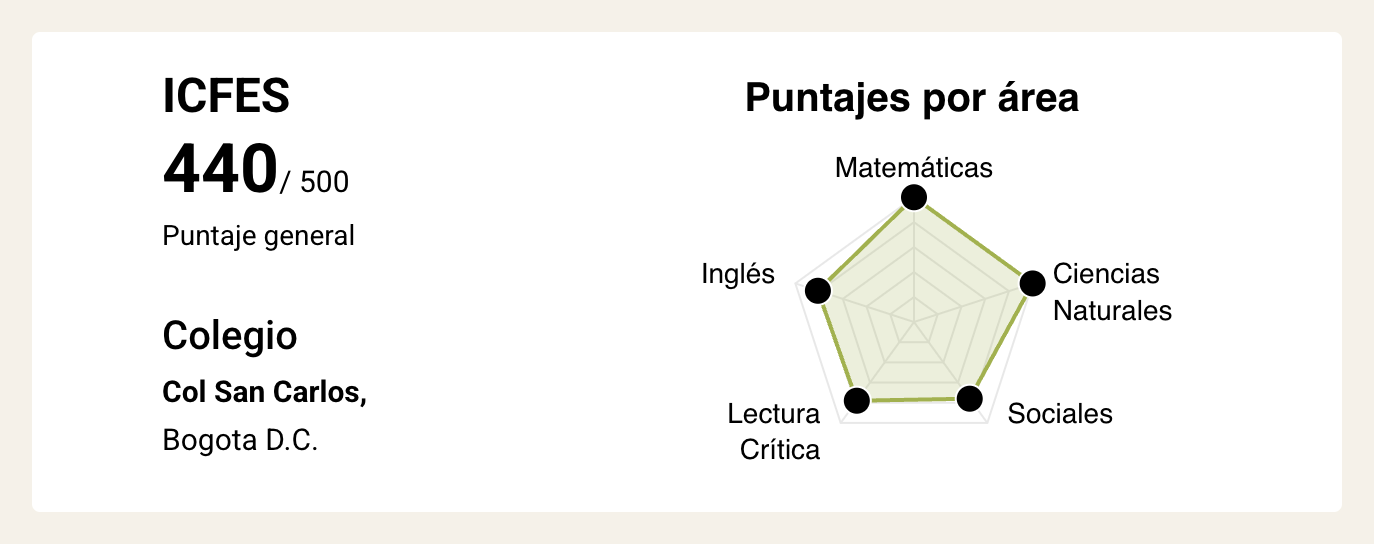
\includegraphics[width=\textwidth]{assets/nes/icfes.png}
	\caption{Resultados del ICFES.}
	\label{fig:icfes}
\end{figure}

\subsubsection{Pestaña de Materias}

La pestaña de Materias presenta un listado de todas las asignaturas que el estudiante ha inscrito a lo largo de su estancia en la Universidad. Consta de dos componentes principales. En la parte superior, mostrada en la figura \ref{fig:filtros_materias}, se encuentra un componente que permite buscar o filtrar materias con facilidad, incluyendo una barra de búsqueda textual y tres filtros: por periodo, por código de área de la materia y por estado de la asignatura (aprobada, retirada, reprobada, pendiente o incompleta). Cada filtro cuenta con un menú desplegable que permite al usuario seleccionar una o varias opciones entre las posibilidades de filtrado. Como ejemplo, la figura \ref{fig:filtro_periodo_materias} muestra el filtro por periodo.

\begin{figure}[H]
	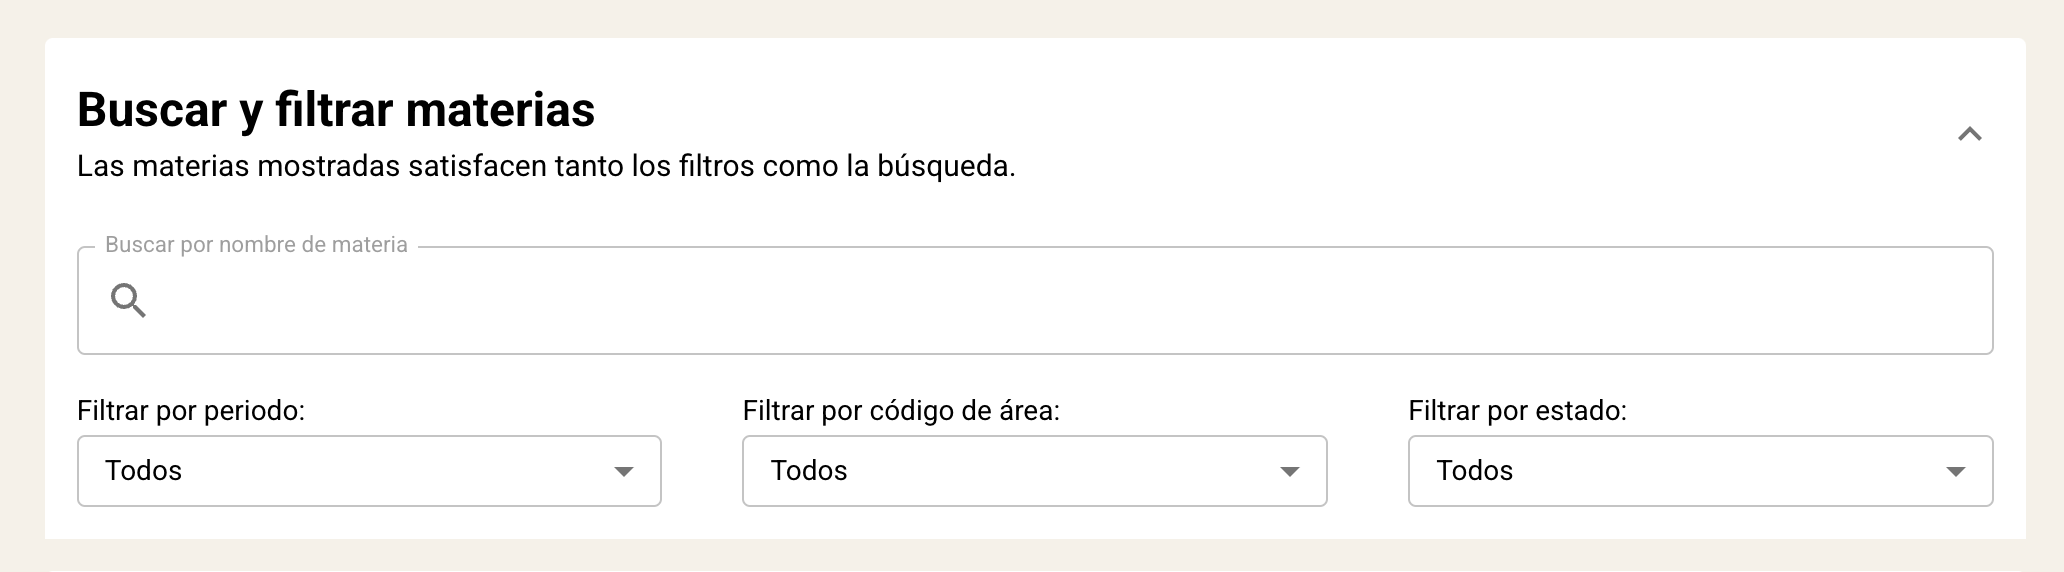
\includegraphics[width=\textwidth]{assets/nes/filtros_materias.png}
	\caption{Componente de búsqueda y filtros de materias.}
	\label{fig:filtros_materias}
\end{figure}

\begin{figure}[H]
	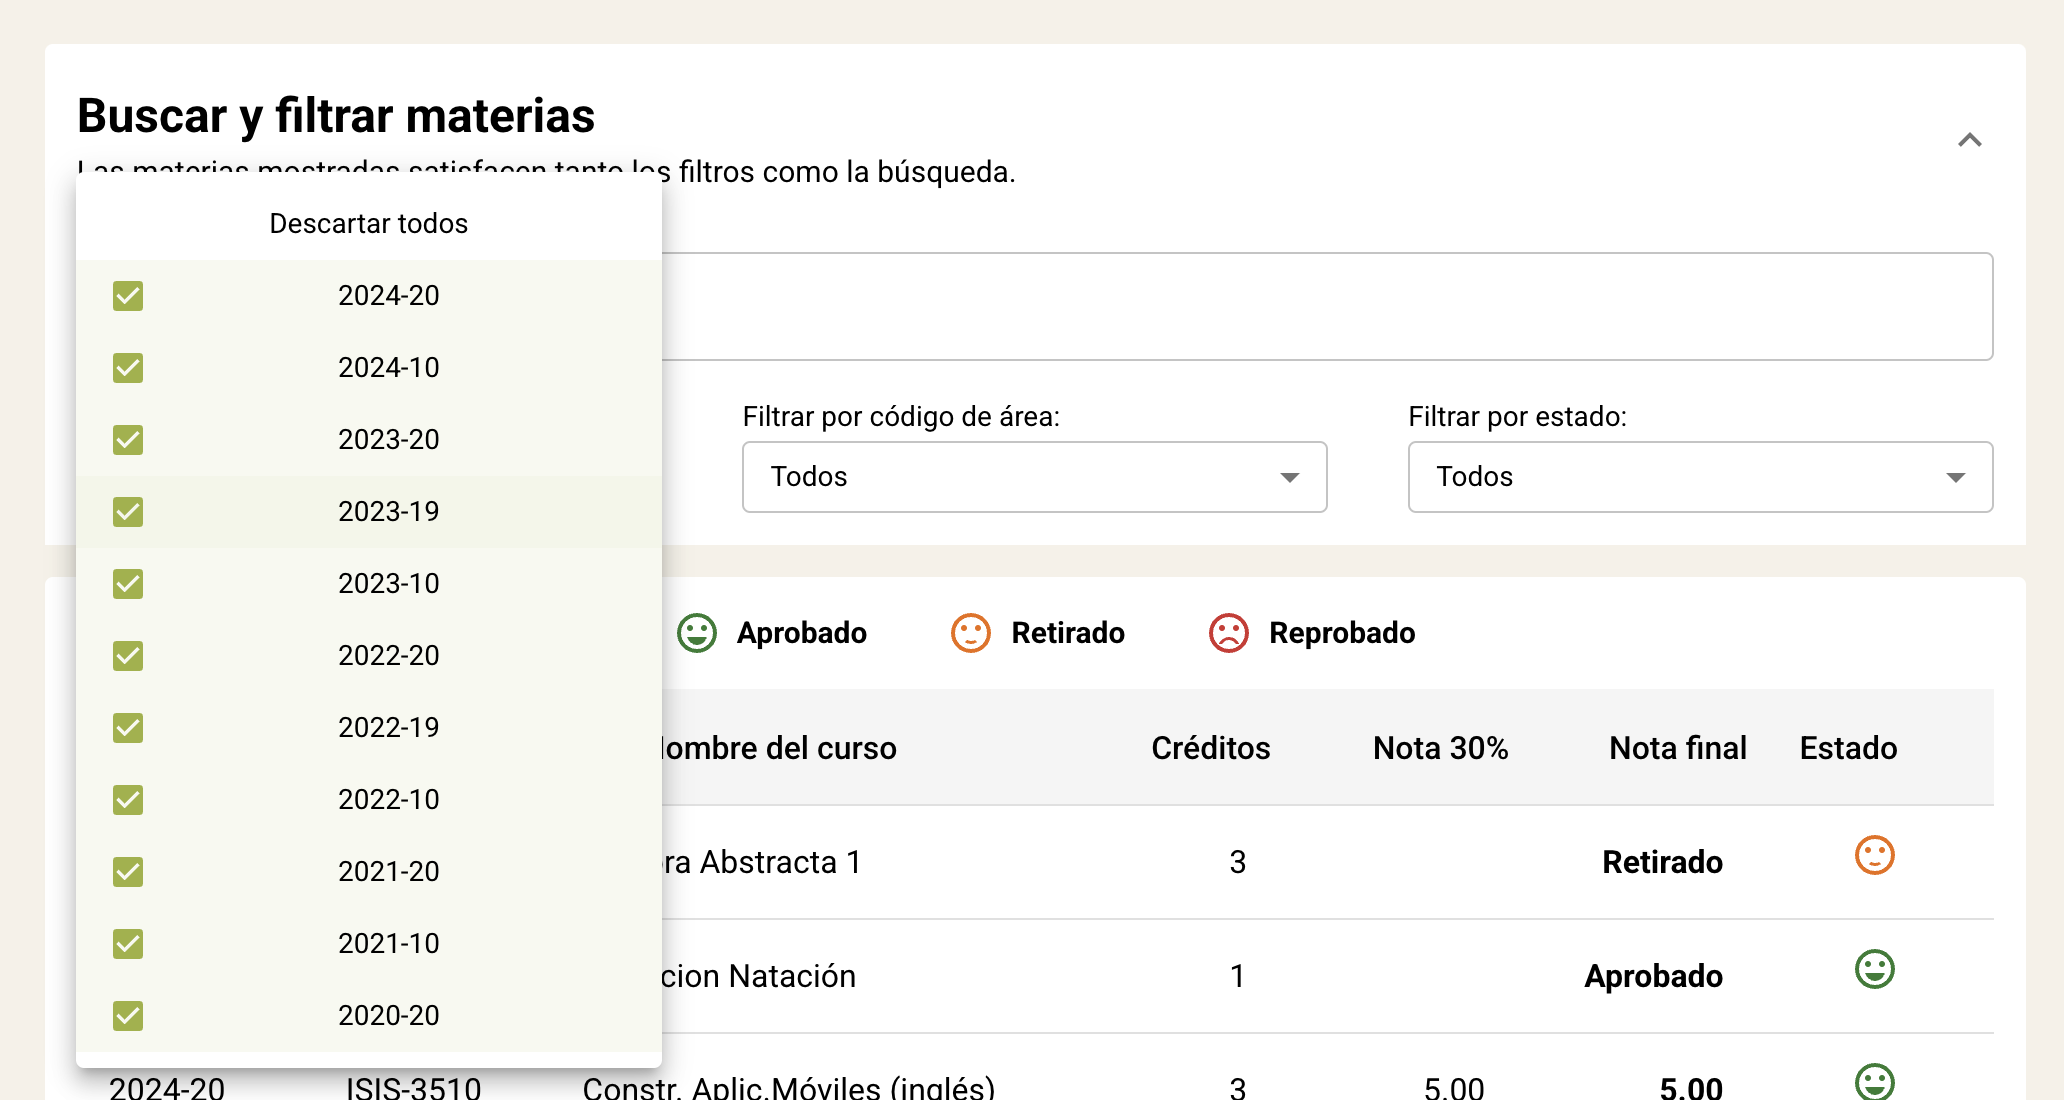
\includegraphics[width=\textwidth]{assets/nes/filtro_periodo_materias.png}
	\caption{Menú desplegable de filtro por periodo en el componente de búsqueda y filtros de materias.}
	\label{fig:filtro_periodo_materias}
\end{figure}

Debajo de ese componente, se encuentra la tabla con el listado de materias, que está en la figura \ref{fig:tabla_materias}. Para cada materia, se muestra el periodo en el que se cursó, el código, el nombre, el número de créditos, la calificación parcial obtenida por el estudiante en el 30\% de la materia, la nota final alcanzada y el estado de la materia. Adicionalmente, las materias que se cursaron de forma virtual están marcadas con un ícono que lo indica. La tabla se puede ordenar por cualquiera de las columnas, permitiendo al usuario visualizar la información de la forma que prefiera, en adición a los filtros y la barra de búsqueda.

\begin{figure}[H]
	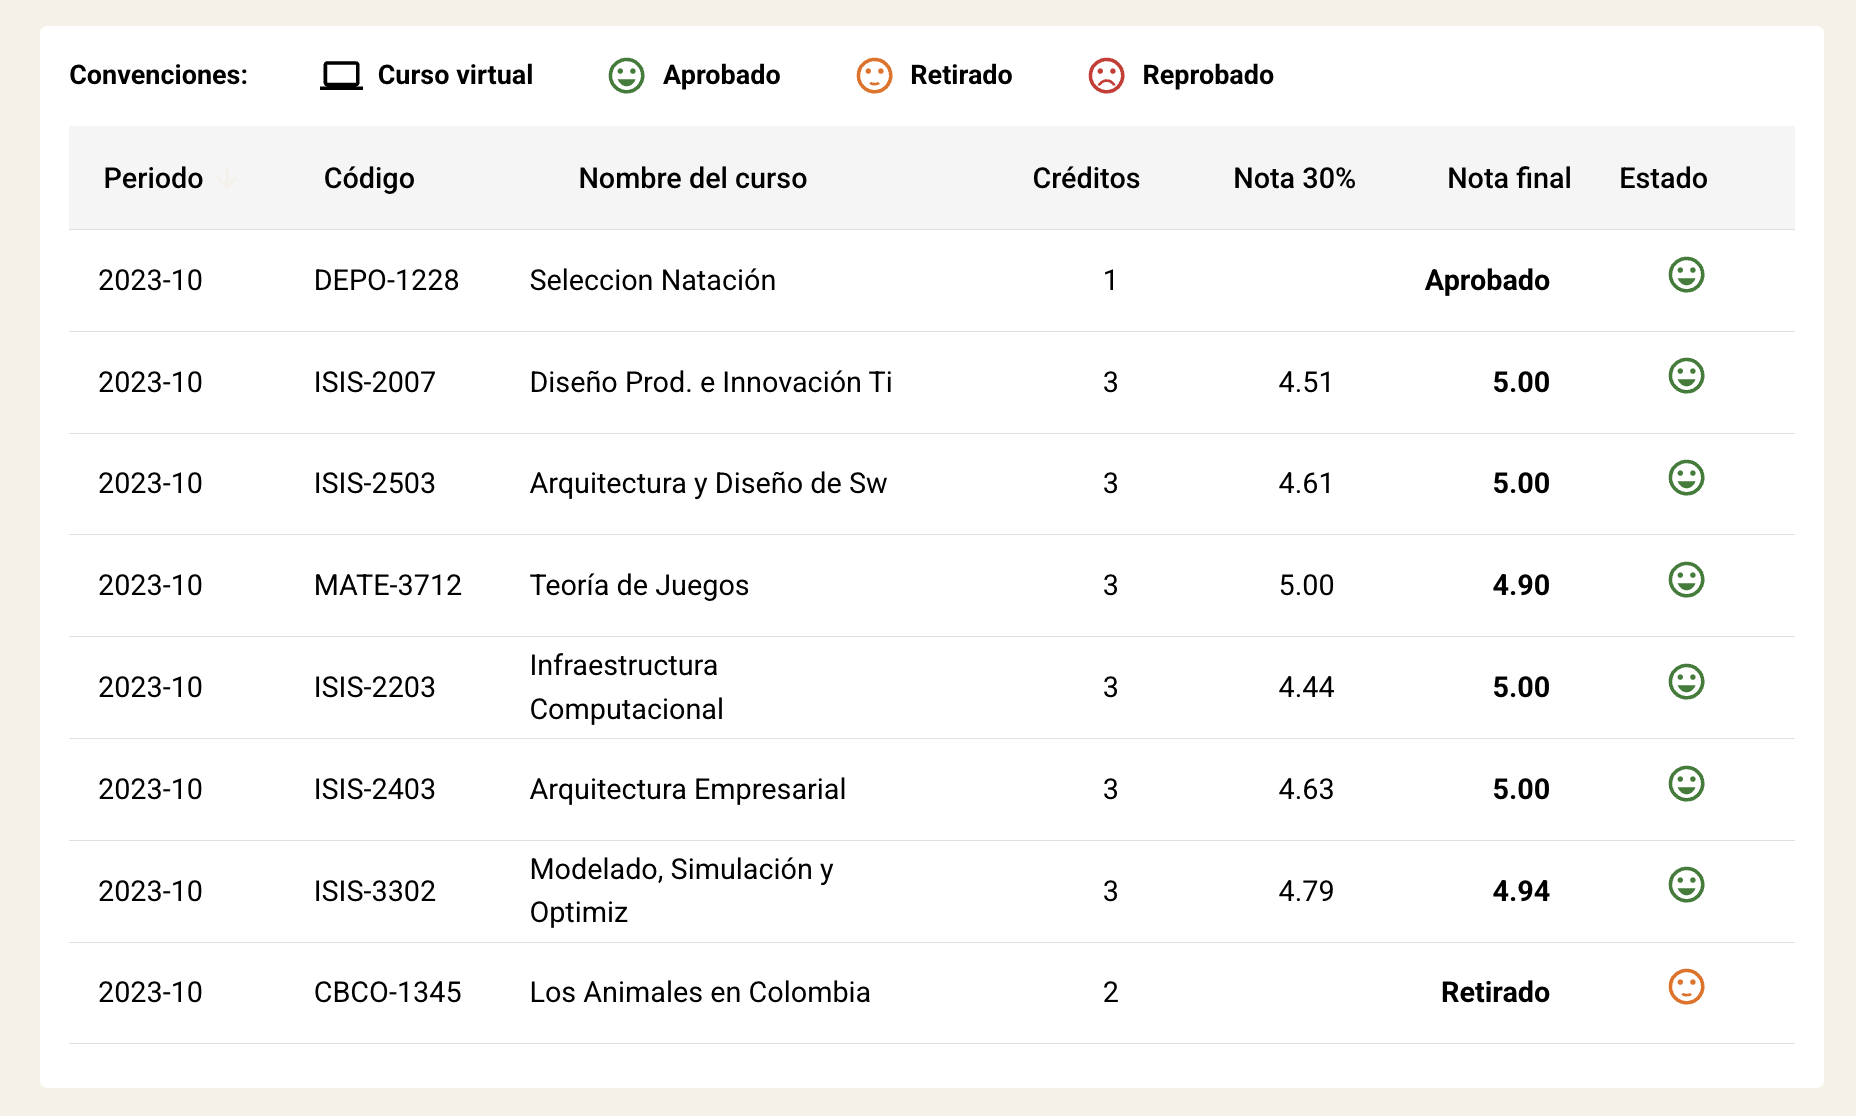
\includegraphics[width=\textwidth]{assets/nes/tabla_materias.png}
	\caption{Tabla de materias inscritas, filtrada para el periodo 2023-10.}
	\label{fig:tabla_materias}
\end{figure}

Esta pestaña permite varios casos de uso distintos sin necesidad de contar con muchos componentes. A continuación, se describen algunos de los más comunes:
\begin{itemize}
	\item Consultar si un estudiante ha cursado o no una materia específica (haciendo uso de la barra de búsqueda) y, en caso de haberla cursado, ver el resultado obtenido.
	\item Visualizar las calificaciones de un estudiante en un área de conocimiento específica, por ejemplo, matemáticas (haciendo uso del filtro por código de área de la materia, en este caso, la opción MATE).
	\item Ver cuántas y cuáles materias han sido reprobadas o retiradas por un estudiante (haciendo uso del filtro por estado de la materia).
	\item Ver las materias que el estudiante cursó en un periodo académico específico y sus resultados, o ver las que se encuentra cursando en el periodo actual (haciendo uso del filtro por periodo).
	\item Consultar todas las materias inscritas por el estudiante en un periodo académico específico.
	\item Conocer las materias en las que el estudiante ha tenido mejor o peor desempeño, ordenando la tabla por la columna de nota final.
\end{itemize}

\subsubsection{Pestaña de Financiación}

La pestaña de Financiación presenta información detallada sobre cómo el estudiante ha financiado sus estudios en la Universidad. Esta pestaña solo es accesible para los directivos de la Universidad, quienes pueden hallarla útil para la toma de decisiones relacionadas con el otorgamiento de apoyos financieros.

La pestaña contiene dos piezas fundamentales de información:
\begin{itemize}
	\item El estrato socioeconómico del estudiante. En Colombia, \say{la estratificación socioeconómica es una clasificación en estratos de los inmuebles residenciales que deben recibir servicios públicos. Se realiza principalmente para cobrar de manera diferencial por estratos los servicios públicos domiciliarios permitiendo asignar subsidios y cobrar contribuciones en esta área.} \cite{estrato}. A causa de eso, es uno de muchos indicadores importantes para determinar la capacidad de pago de un estudiante y, por ende, su necesidad de apoyo financiero.
	\item Un gráfico de barras apiladas con la distribución de la financiación del estudiante en cada periodo académico en el que se ha matriculado. Las barras se dividen en segmentos que representan las distintas fuentes de financiación, como becas, créditos, ahorros, recursos propios, entre otros. Cada segmento se colorea de forma distinta y se etiqueta con el porcentaje de financiación que representa para el periodo en cuestión. La altura de la barra representa el total de la financiación en cada periodo académico, que no necesariamente corresponde al 100\% de la matrícula, pues el estudiante puede haber cursado matrículas parciales.
\end{itemize}
Un ejemplo de la pestaña de Financiación se muestra en la figura \ref{fig:financiacion}.

\begin{figure}[H]
	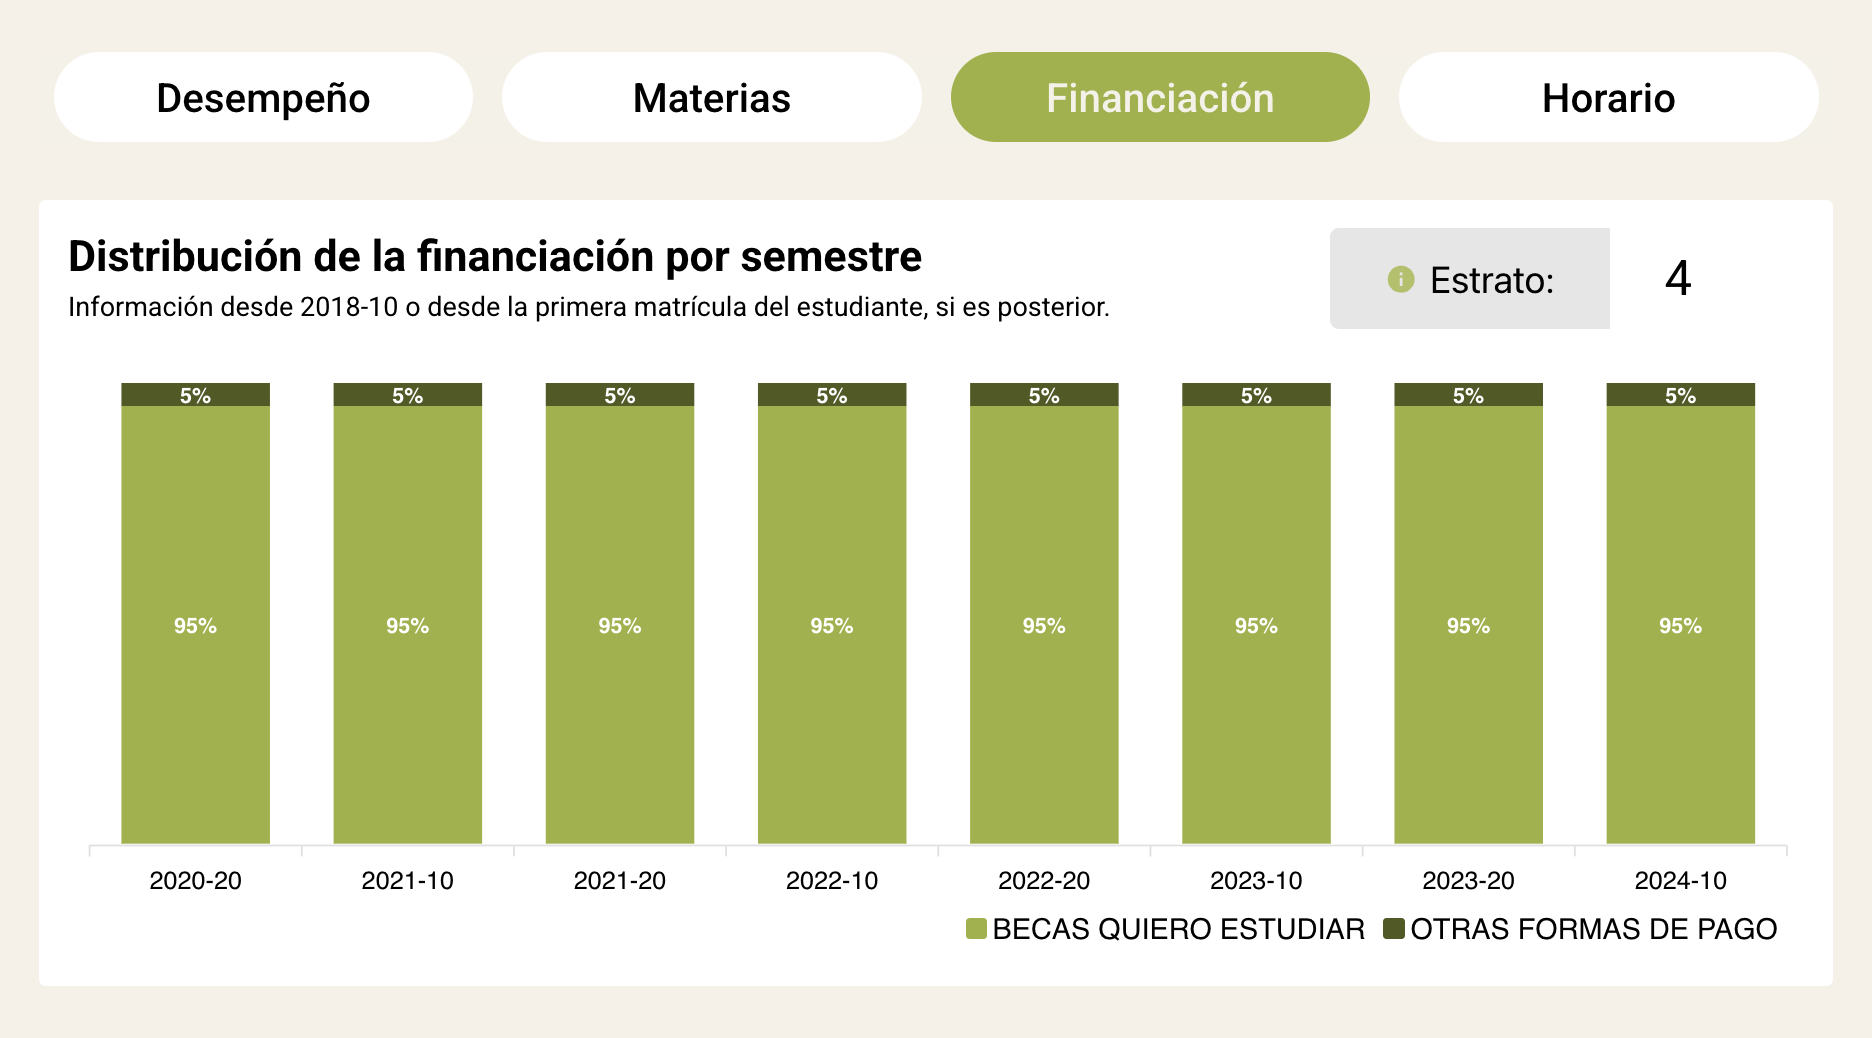
\includegraphics[width=\textwidth]{assets/nes/financiacion.png}
	\caption{Pestaña de Financiación.}
	\label{fig:financiacion}
\end{figure}

\subsubsection{Pestaña de Horario}

La pestaña de Horario presenta el horario de clases del estudiante en el momento de la consulta. El horario se muestra en un formato clásico de horario de clases, como se puede evidenciar en la figura \ref{fig:horario}, donde cada columna representa un día de la semana y cada fila representa una franja de media hora. Cada celda de la tabla contiene la información de la materia que el estudiante tiene programada en ese día y a esa hora.

\begin{figure}[H]
	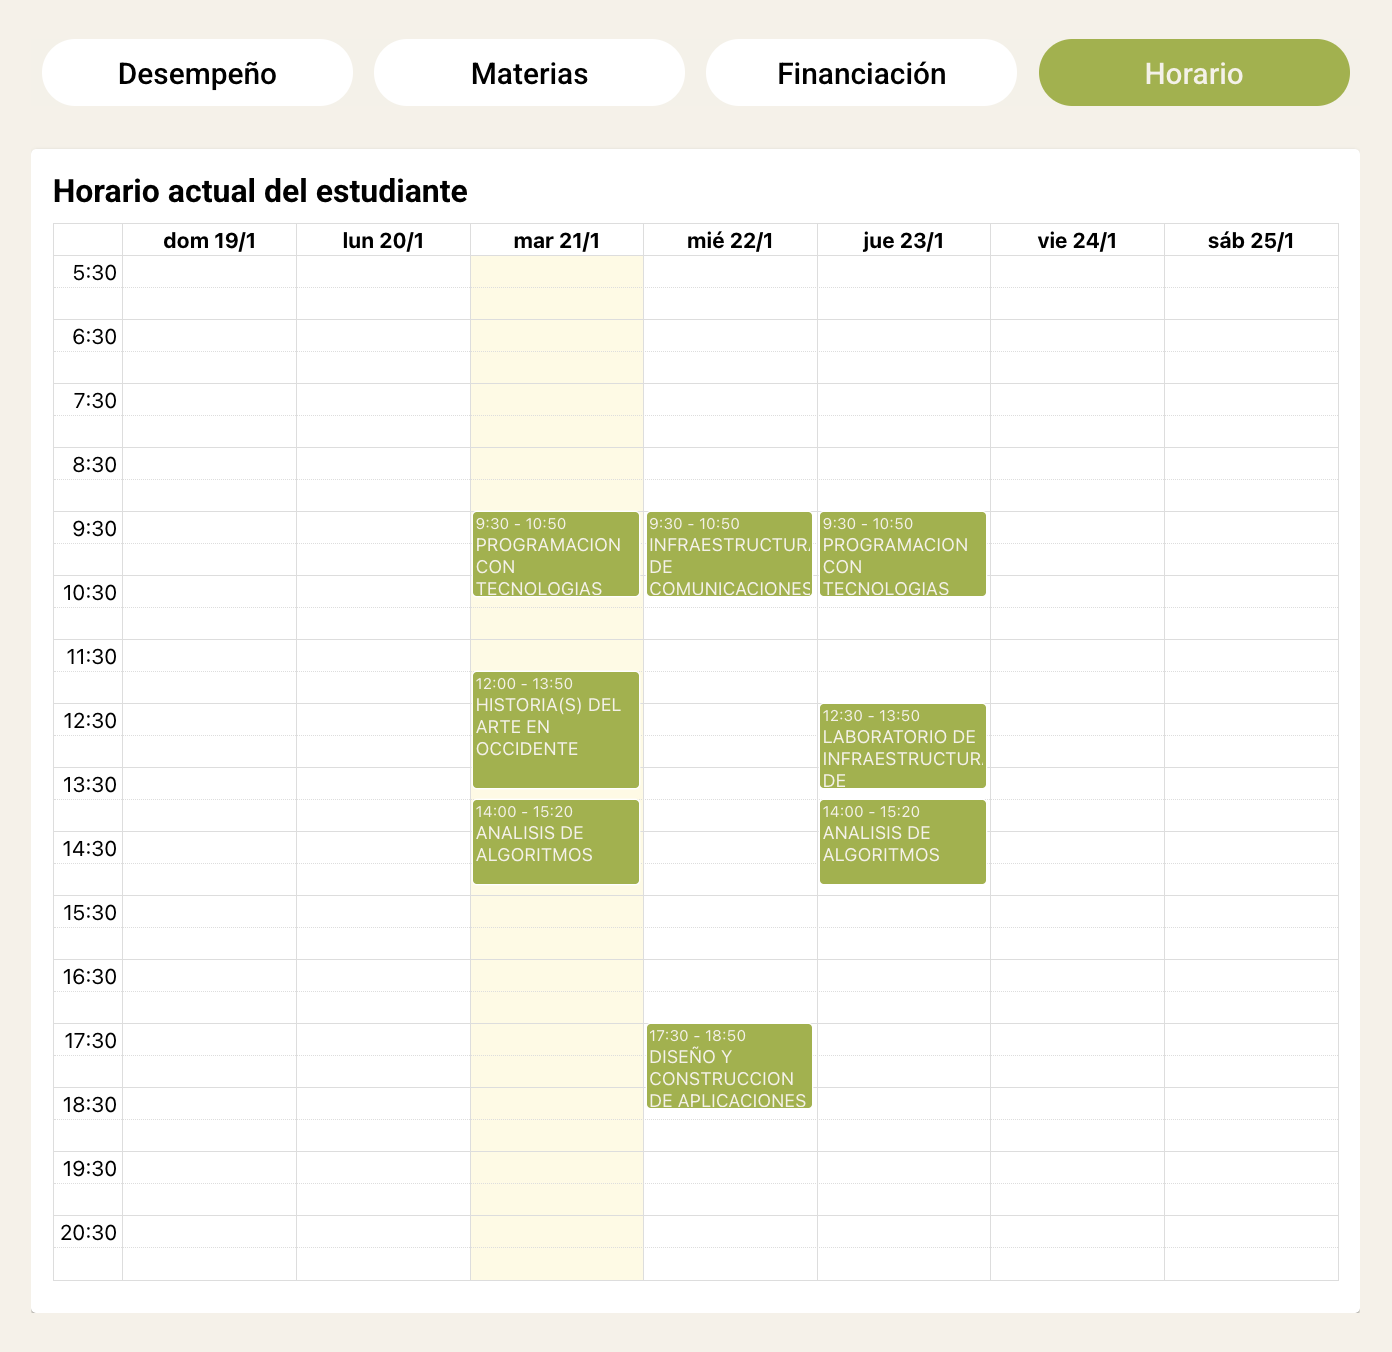
\includegraphics[width=\textwidth]{assets/nes/horario.png}
	\caption{Horario de clases de un estudiante anónimo.}
	\label{fig:horario}
\end{figure}

Al pulsar en una celda de la tabla, se despliega una ventana emergente con información detallada de la materia, incluyendo el código de la materia, el nombre de la materia, el nombre del profesor, el salón de clases y el tipo de clase (magistral, complementaria, laboratorio, taller, entre otros). En caso de que el estudiante tenga una materia virtual programada, aparece un ícono que lo indica. Se muestra la información de una materia en la figura \ref{fig:detalle_horario}.

\begin{figure}[H]
	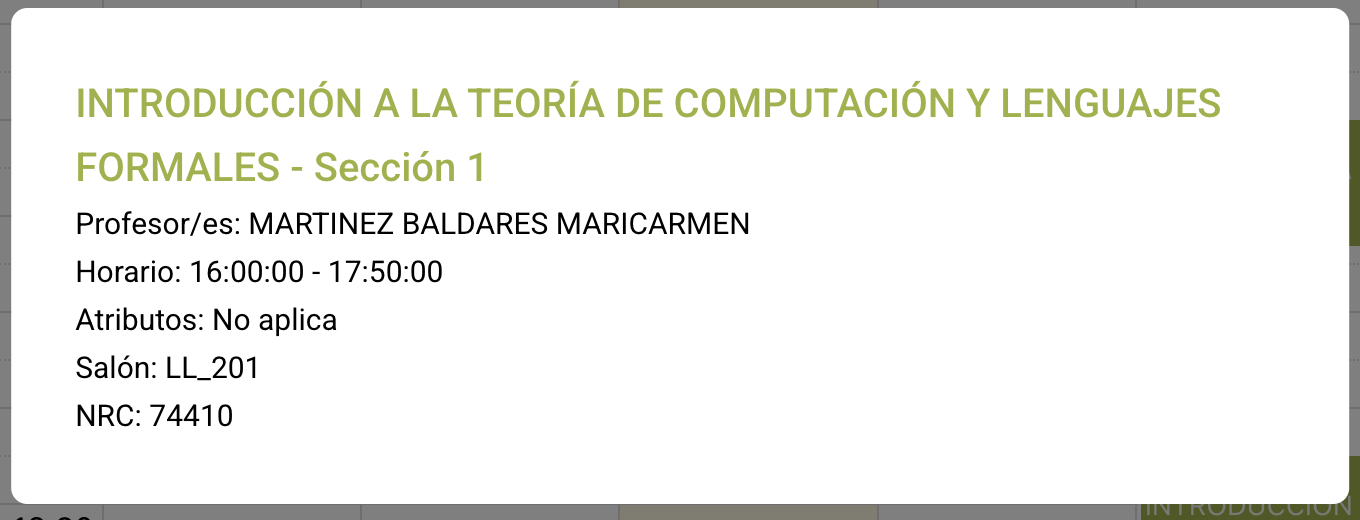
\includegraphics[width=\textwidth]{assets/nes/detalle_horario.png}
	\caption{Detalle de una materia en el horario de un estudiante anónimo.}
	\label{fig:detalle_horario}
\end{figure}

Esta pestaña es naturalmente útil para los estudiantes, particularmente al inicio de cada semestre, cuando deben organizar su tiempo y coordinar sus actividades. Sumado a eso, la pestaña es de gran utilidad para los profesores, quienes pueden visualizar el horario de sus estudiantes y coordinar reuniones, tutorías y otros eventos con ellos. Para servir a ese fin, el horario cambia dinámicamente cada semana como respuesta a modificaciones en los horarios de clase, por ejemplo, a causa de días festivos o de eventos organizados por la Universidad.

\subsubsection{Información específica para estudiantes en riesgo académico}

En el diseño del Perfil del estudiante, se incorporó una funcionalidad específica para alertar sobre estudiantes que cumplen algún criterio de riesgo académico. Actualmente, se identifican cinco criterios de riesgo académico, que son los siguientes:
\begin{itemize}
	\item El estudiante está en segundo semestre y tiene un PGA entre 3.00 y 3.30.
	\item El estudiante está en tercer semestre o superior y tiene un PGA entre 3.25 y 3.50.
	\item El estudiante pagó matrícula completa, pero tiene inscritos menos de 13 créditos.
	\item El estudiante ha retirado $x$ materias en el semestre actual.
	\item El estudiante va perdiendo $x$ materias al corte del 30\%.
\end{itemize}

En los últimos dos criterios, la $x$ corresponde al número de materias en cuestión, de acuerdo con la realidad del estudiante. Esos dos criterios se muestran únicamente en caso de que la cantidad de materias sea de 3 o más. Ese valor es parametrizable y puede ser ajustado a conveniencia por los directivos de la Universidad.

En caso de que el alumno satisfaga alguno de esos criterios, se presenta un mensaje de alerta en la parte superior de la pestaña de Desempeño, indicando con gran visibilidad el riesgo académico correspondiente. La figura \ref{fig:riesgo_academico} presenta un ejemplo de un estudiante con riesgo académico. Estos riesgos se muestran a cualquier profesor o administrativo que consulte el perfil, así como también al estudiante cuando consulta su propio perfil.

\begin{figure}[H]
	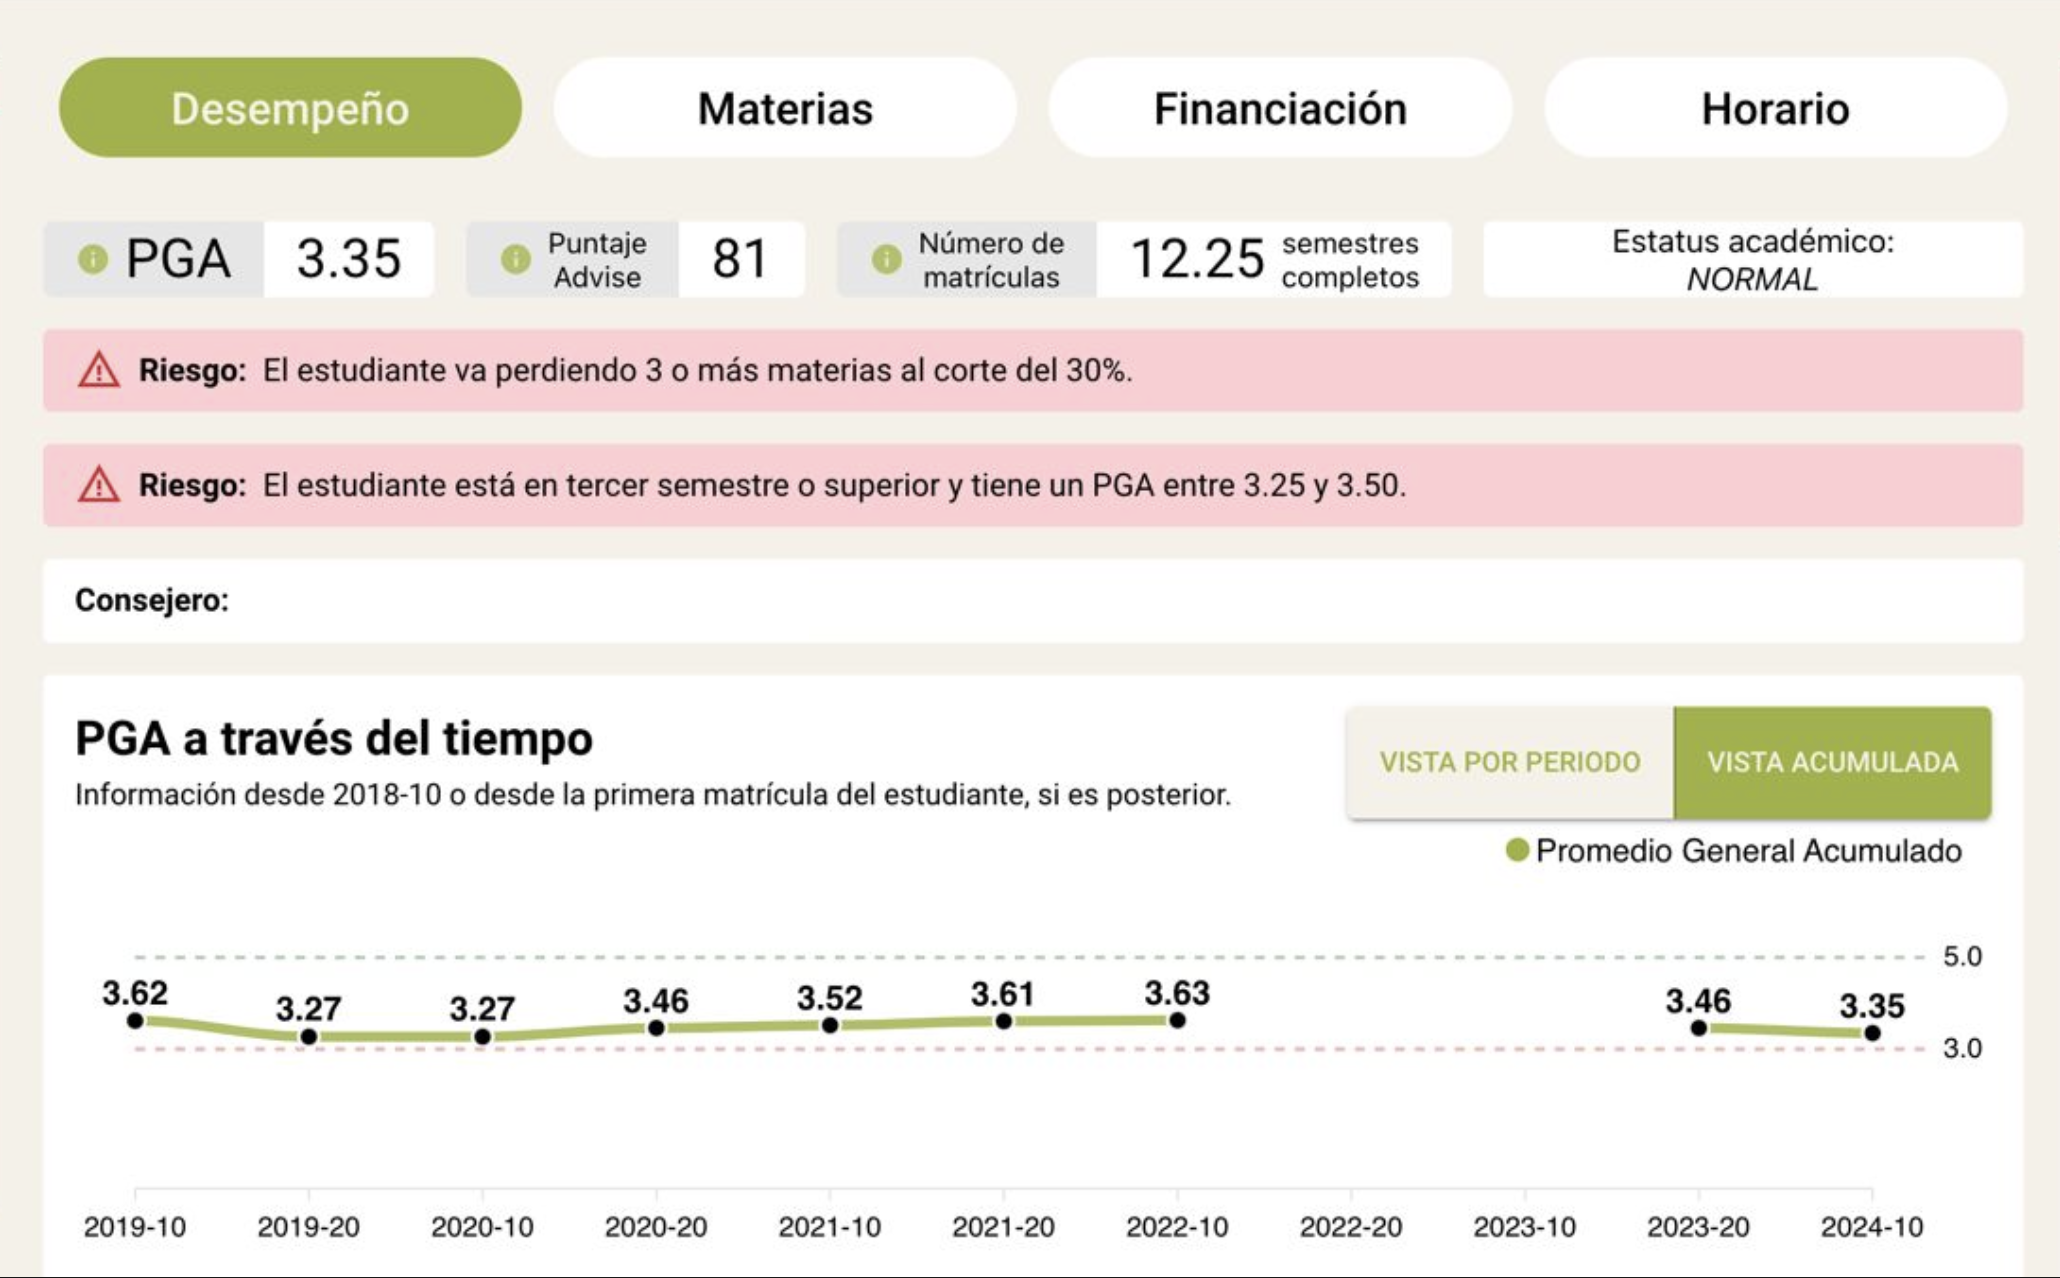
\includegraphics[width=\textwidth]{assets/nes/riesgo_academico.png}
	\caption{Mensaje de alerta de riesgo académico en el perfil de un estudiante anónimo.}
	\label{fig:riesgo_academico}
\end{figure}

\subsubsection{Información específica para estudiantes graduados}

En el Perfil del estudiante se agregó información específica para estudiantes graduados. En la pestaña de Desempeño, se presenta un mensaje que exalta el logro de haberse graduado y exhibe el título obtenido, con el mes y año en el que se obtuvo. En caso de que el alumno haya completado alguna opción académica, se registra la compleción de la opción, como se puede ver en la figura \ref{fig:graduado}.

\begin{figure}[H]
	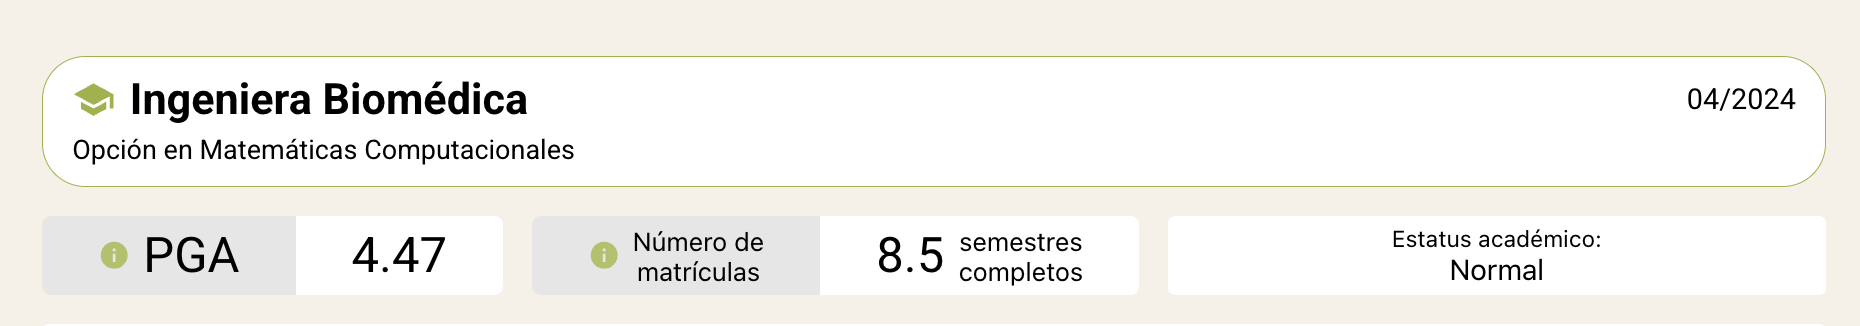
\includegraphics[width=\textwidth]{assets/nes/graduado.png}
	\caption{Mensaje de graduación en el perfil de un estudiante anónimo.}
	\label{fig:graduado}
\end{figure}

Sumado a eso, en caso de que haya sido galardonado durante la carrera o se haya graduado con honores, se resalta ese logro. Un ejemplo de un estudiante graduado con honores está en la figura \ref{fig:graduado_honores}.

\begin{figure}[H]
	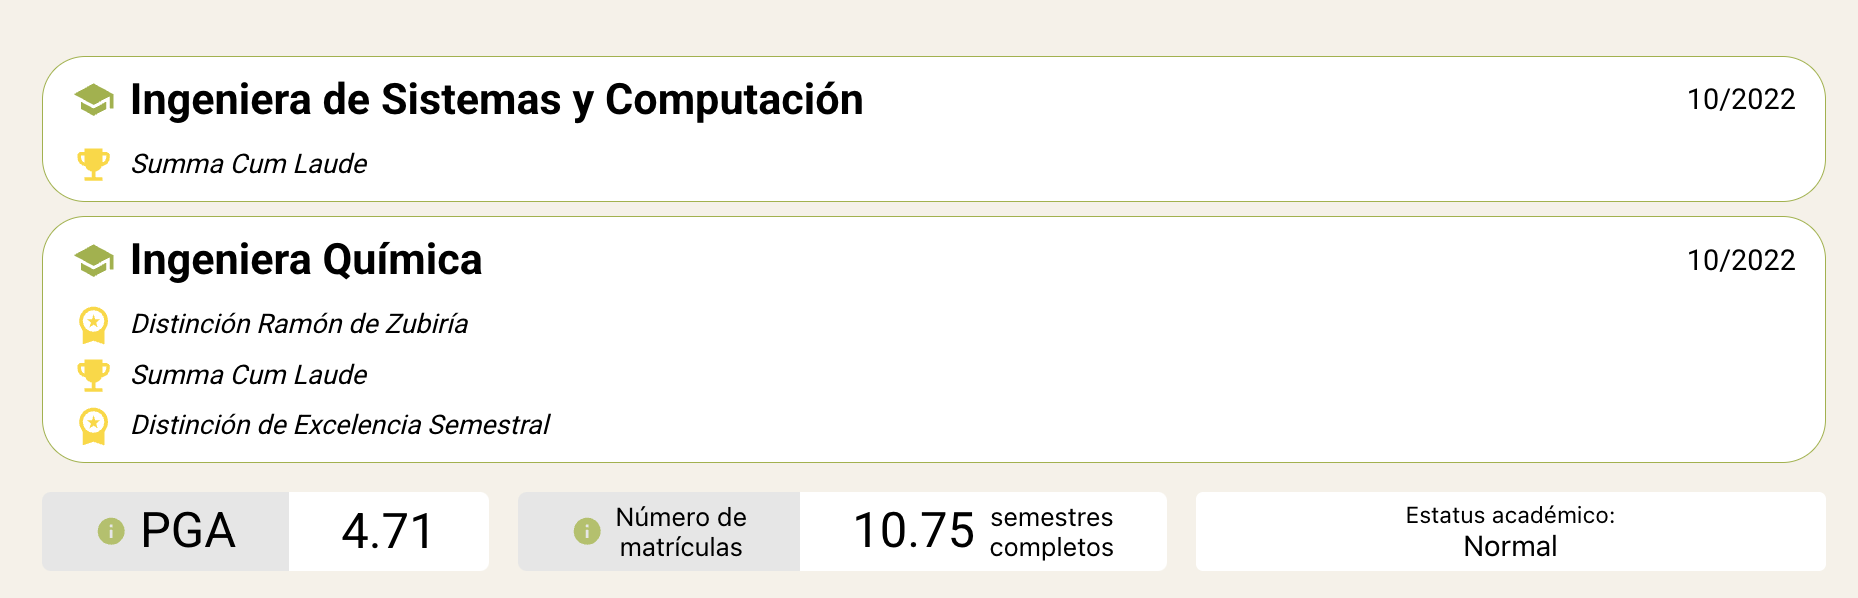
\includegraphics[width=\textwidth]{assets/nes/graduado_honores.png}
	\caption{Mensaje de graduación con honores en el perfil de un estudiante anónimo.}
	\label{fig:graduado_honores}
\end{figure}

\chapter{Conclusión}
\label{ch:conclusion}

Este proyecto ha explorado de manera exhaustiva el desarrollo del módulo de Perfil del estudiante, integrado dentro de la plataforma web \gls{NES}, a través de la arquitectura clásica de tres capas: datos, lógica y presentación. Cada una de estas capas fue abordada con detalle, tanto desde su diseño conceptual como desde su implementación técnica, utilizando tecnologías modernas y las mejores prácticas de desarrollo de software.

La capa de datos constituye el cimiento del sistema, responsable de la extracción, transformación y carga (\gls{ETL}) de información relevante proveniente de diversas fuentes institucionales. La calidad y consistencia de los datos se garantizan mediante un pipeline de analítica notablemente robusto, implementado en cuadernos de \gls{Jupyter} en \gls{Python}, con la imprescindible colaboración de Santiago Martínez Novoa.

La capa de lógica es el núcleo del sistema, encargada de procesar los datos y exponerlos a través de un \gls{API REST}. Implementada con \gls{FastAPI}, esta capa utiliza esquemas y modelos bien definidos, asegurando que los datos fueran accesibles de manera eficiente y segura. Su diseño asegura la independencia entre capas, permitiendo que el \gls{API} sea escalable, mantenible y fácil de integrar con otros sistemas.

En este punto se contemplaron preocupaciones a nivel de seguridad que nacen naturalmente a raíz de la sensibilidad de los datos manejados. Además de la seguridad manejada a nivel de software, la información se almacenó en una base de datos \gls{PostgreSQL}, alojada en una máquina que está protegida del internet, separada físicamente mediante \textit{air gapping}.

La capa de presentación es la cara del sistema. Ofrece una interfaz de usuario interactiva, accesible y amigable, desarrollada con \gls{React} y \gls{TypeScript}. Diseñada para satisfacer las necesidades de estudiantes, profesores y directivos, esta capa organiza la información en pestañas intuitivas y utiliza herramientas visuales como gráficos y tablas interactivas que facilitan la navegación y comprensión de los datos.

El alcance de este proyecto no se limitó a la construcción técnica de estas tres capas. También incluyó el despliegue en un entorno real de producción, enfrentando retos como la integración con otros módulos de \gls{NES}, la gestión de seguridad de la información y la optimización del rendimiento. Esto convierte al Perfil del estudiante en un proyecto integral, que abarca todos los aspectos del ciclo de vida del desarrollo de software. Es razonable afirmar que cada una de las capas podría ser, por sí sola, el tema central de una tesis completa. Este trabajo, sin embargo, logró integrarlas en un producto funcional que ya está generando un impacto tangible en la comunidad universitaria.

La esencia de la ingeniería radica en poner el conocimiento técnico al servicio a la sociedad. Da gran orgullo percatarse de que este proyecto cumple con ese propósito. El Perfil del estudiante no solo mejora la vida académica y profesional de estudiantes, profesores y directivos, sino que también fortalece el rol de la Universidad de los Andes como una institución líder en Colombia. Al facilitar la toma de decisiones informadas, apoyar a los estudiantes en riesgo académico y optimizar el uso de recursos, este sistema contribuye al desarrollo de la comunidad uniandina y, en última instancia, al progreso del país.

Finalmente, resulta simbólico observar que la palabra más frecuente en este documento es \say{estudiante}. Esto refleja el espíritu central del proyecto: un sistema concebido por un estudiante, con el apoyo de un equipo de estudiantes y diseñado para el beneficio del estudiantado.

Ojalá que este software continúe siendo, por mucho tiempo, un aporte tangible al bienestar de todos en la Universidad de los Andes.

\appendix
\chapter{Contribuciones al CAPP}

Este apéndice describe las contribuciones realizadas al \gls{CAPP} durante el desarrollo de este proyecto. En particular, se detallan los recursos expuestos por la \gls{API REST} para consumo exclusivo del \gls{CAPP}, a petición de Daniel Arango Cruz y Marilyn Stephany Joven Fonseca, quienes lideran el desarrollo de aquel proyecto.

\section{Contexto}

El \gls{CAPP} es un sistema que permite a los estudiantes de pregrado de la Universidad de los Andes visualizar su progreso académico. Su propósito principal es determinar si un estudiante ha cumplido con los requisitos mínimos para graduarse de un programa académico. Para ello, el \gls{CAPP} se conecta con diversas fuentes de datos, entre ellas, con el \gls{API REST} diseñado y desarrollado en este proyecto.

\section{Recursos expuestos}

Los recursos provistos fueron diseñados específicamente para el \gls{CAPP} ante solicitud de los desarrolladores de ese proyecto. Se solicitó que la nomenclatura para los recursos y sus atributos fuera en español, en lugar de inglés, como se había manejado en el resto de la \gls{API REST}.

A causa de eso y como forma de separación semántica, se decidió agrupar los \textit{endpoints} bajo el prefijo \lstinline|/capp/|. La tabla \ref{tab:capp_api_resources} detalla los \textit{endpoints} expuestos por la \gls{API REST} para el \gls{CAPP}.

\begin{longtblr}[
		caption = {Recursos expuestos por la \gls{API REST} para el  \gls{CAPP}},
		label = {tab:capp_api_resources},
	]{
		colspec = {X[4,l] X[4,l] X[5,l] X[4,l] X[4,l]}
	}
	\hline
	\textbf{Método HTTP} & \textbf{URL}                                             & \textbf{Descripción}                                                                      & \textbf{Cuerpo de la petición} & \textbf{Respuesta}                                                                 \\ \hline
	\lstinline|GET|      & \lstinline|/capp/materias/estudiante/:codigo_estudiante| & Obtiene todas las materias aprobadas por un estudiante en sus estudios de pregrado.       & --                             & Lista de objetos \lstinline|Materia| con las materias aprobadas por el estudiante. \\
	\lstinline|GET|      & \lstinline|/capp/materia/:codigo_materia |               & Obtiene la información básica de una materia a partir de su código.                       & --                             & Objeto \lstinline|Materia| correspondiente al código.                              \\
	\lstinline|PUT|      & \lstinline|/capp/materias/|                              & Obtiene la información básica de múltiples materias a partir de una lista de sus códigos. & Lista de códigos de materias   & Lista de objetos \lstinline|Materia| correspondientes a los códigos provistos.     \\
	\lstinline|GET|      & \lstinline|/capp/estudiante/programa/|                   & Obtiene la información de los programas académicos cursados por el estudiante.            & --                             & Lista de nombres de los programas académicos, ordenados desde el principal.        \\
	\hline
\end{longtblr}

El recurso \verb|Materia| mencionado en la tabla es una representación simplificada de una materia, que contiene la información mínima necesaria para el \gls{CAPP}. La figura \ref{lst:subject_capp} muestra un ejemplo de esta representación.

\begin{figure}[h]
	\centering
	\begin{minted}{json}
{
  "codigo_curso": "MATE",
  "numero_curso": "1104",
  "numero_creditos": 3,
  "nombre_curso": "TEORIA DE GRAFOS",
  "atributo_sec": "",
  "periodo": 202320
}
  \end{minted}
	\caption{Ejemplo de representación del recurso \lstinline|Materia| para el \gls{CAPP}}
	\label{lst:subject_capp}
\end{figure}

\section{Consideraciones finales}

Las contribuciones realizadas al \gls{CAPP} fueron diseñadas y desarrolladas en colaboración con los líderes de ese proyecto. Se espera que estas contribuciones sean de utilidad para el desarrollo del \gls{CAPP} y que permitan a los estudiantes de pregrado de la Universidad de los Andes visualizar su progreso académico de manera más eficiente y efectiva.


\printglossary
\addcontentsline{toc}{chapter}{Glosario}

\printbibliography
\addcontentsline{toc}{chapter}{Bibliografía}

\end{document}

